\subsection*{Measured raw data}
\setcounter{topnumber}{10}
\setcounter{bottomnumber}{10}
\setcounter{totalnumber}{10}
\renewcommand{\topfraction}{1}
\renewcommand{\bottomfraction}{1}
%\renewcommand{\textfraction}{0.05}
\renewcommand{\floatpagefraction}{1}
%%%%%%%%%%%%%%%%%%%%%%%%%%%%%%%%%%%%
%%% BSA at Vc = 2.5 ml/min
%%%%%%%%%%%%%%%%%%%%%%%%%%%%%%%%%%%%%
\newcommand{\subFigSize}{0.45\linewidth}
%\newcommand{\vertDist}{\vspace*{-1.5ex}}
\begin{figure}[H]
  \begin{center}
    \begin{subfigure}{\subFigSize}
    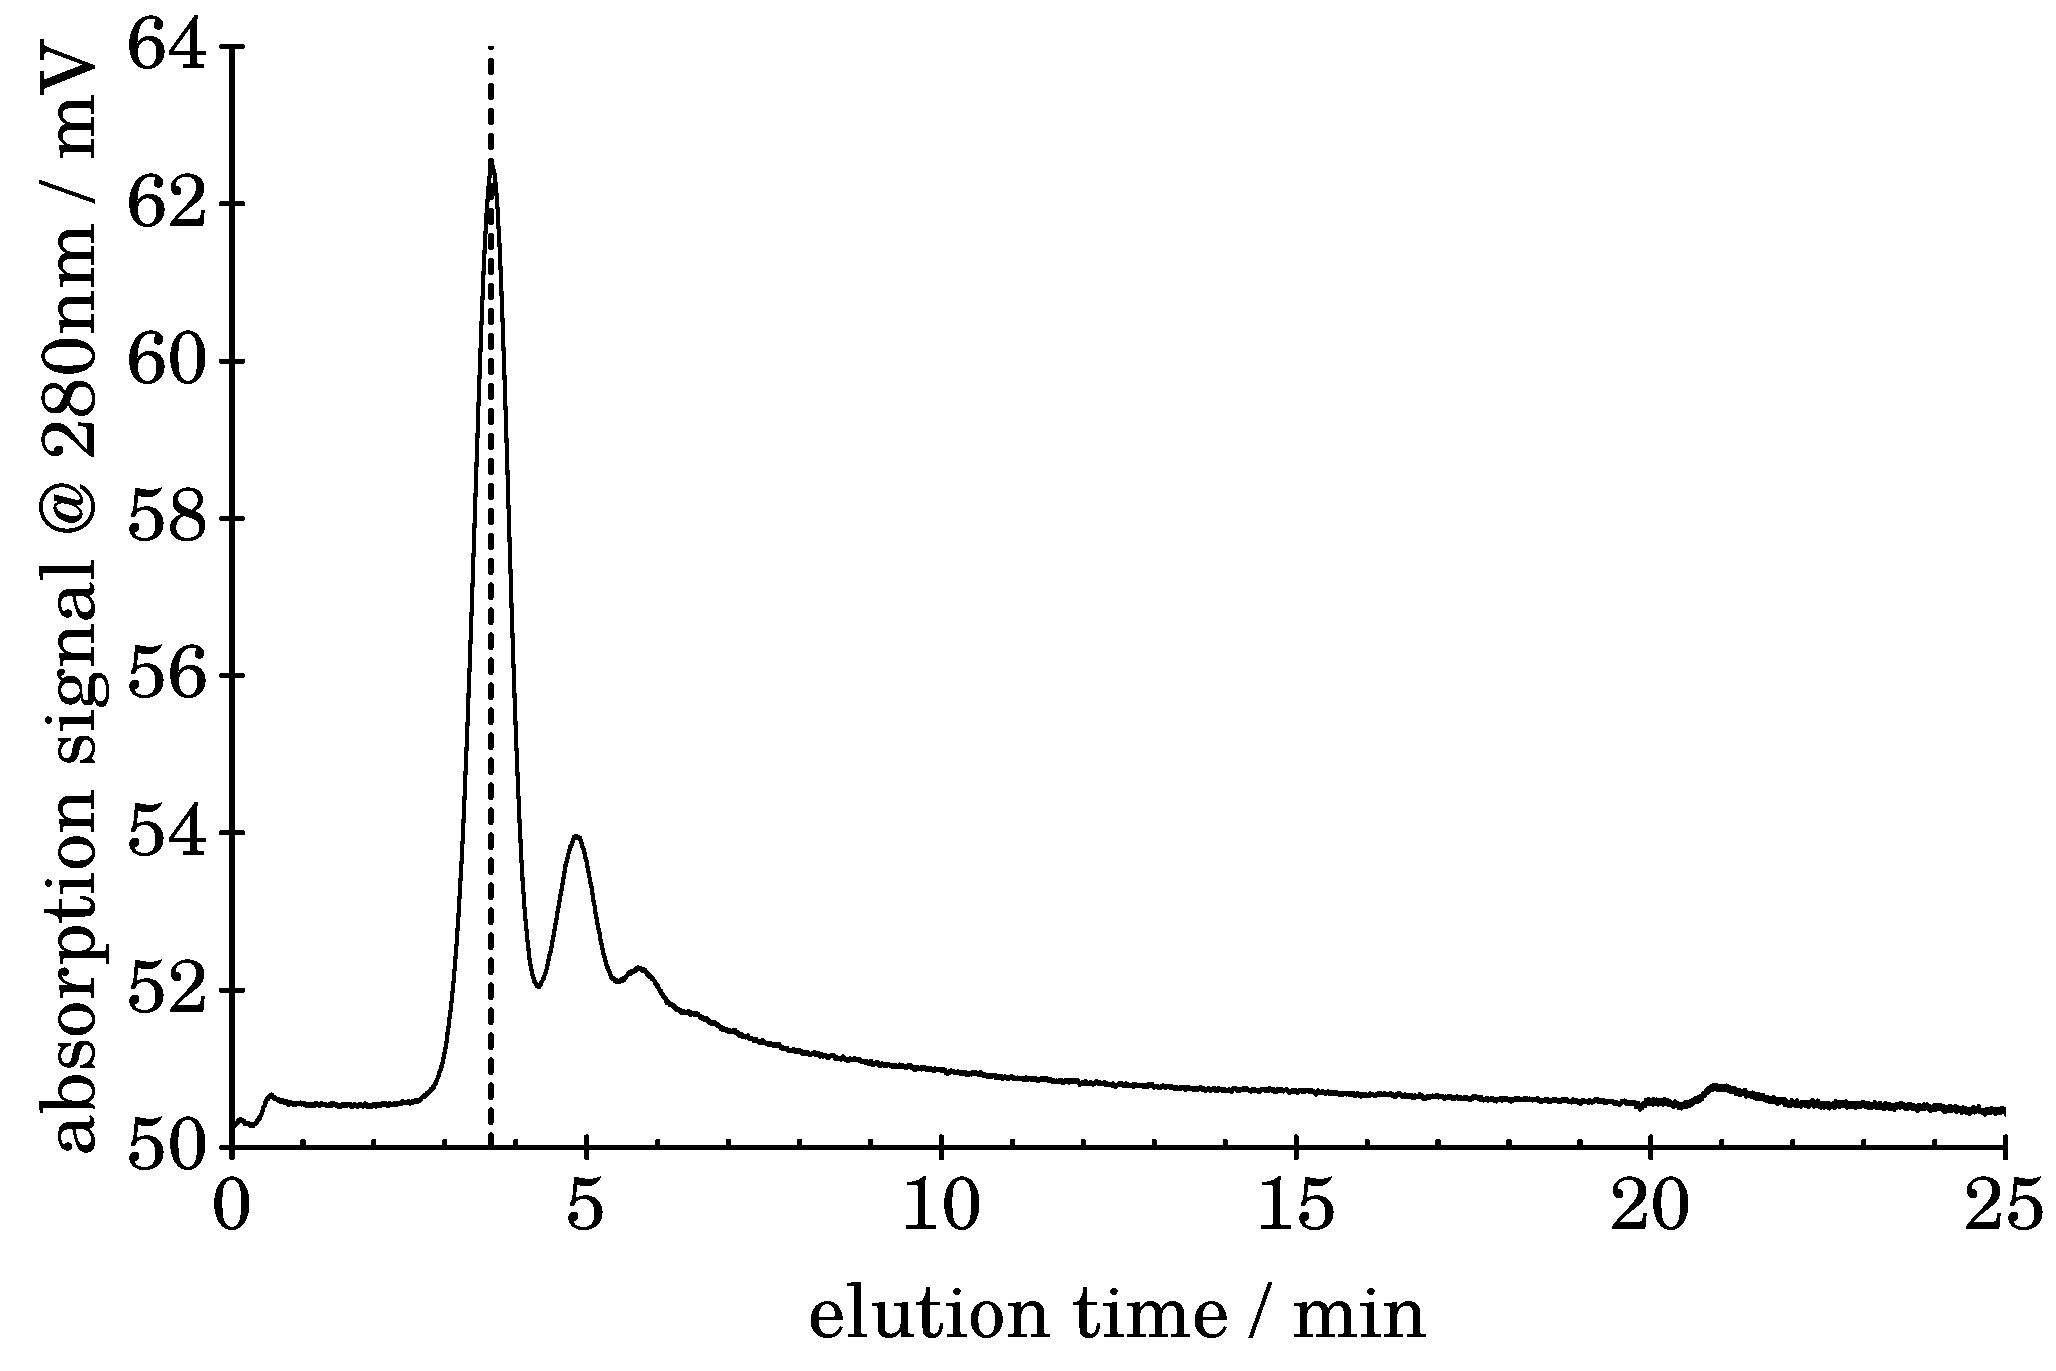
\includegraphics[width=\linewidth]{./images/data/img_BSA_VC_2_5_r1_te.pdf}
      \subcaption{Position of $\te$, replicate 1.}
      \label{subfig:raw_BSA2_5_r1_te}
    \end{subfigure}
      \begin{subfigure}{\subFigSize}
    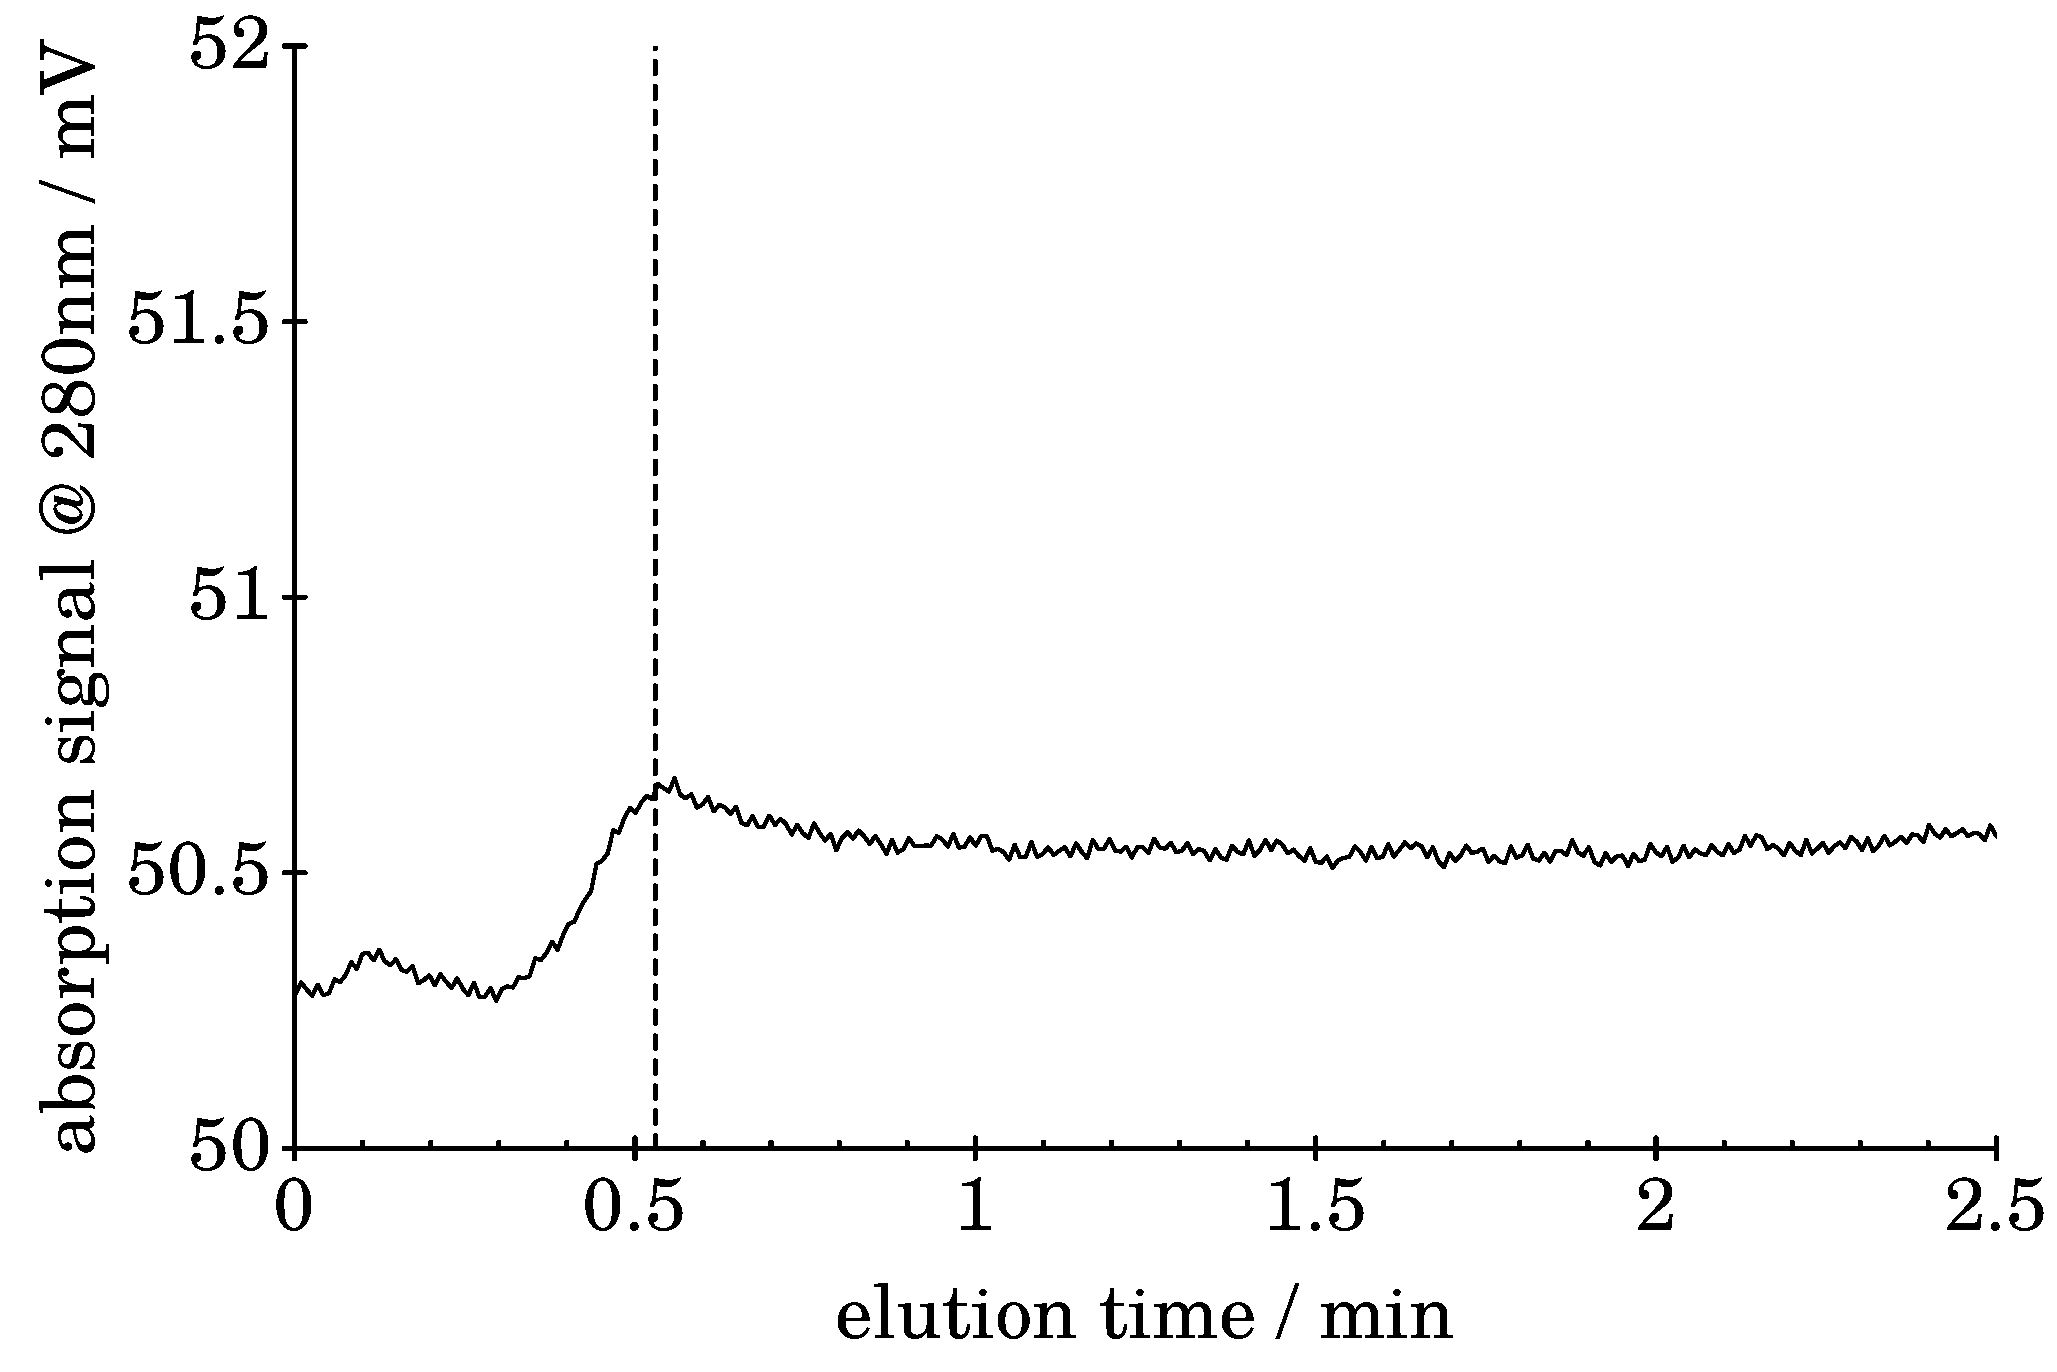
\includegraphics[width=\linewidth]{./images/data/img_BSA_VC_2_5_r1_t0.pdf}
    \subcaption{Detailed starting section of fractogram \ref{subfig:raw_BSA2_5_r1_te};
      Position of $\tvoid$, replicate 1.}
  \end{subfigure}
  \\\vspace*{.5em}
  %%%%%%%%%%%%%%%%%%%%%
      \begin{subfigure}{\subFigSize}
    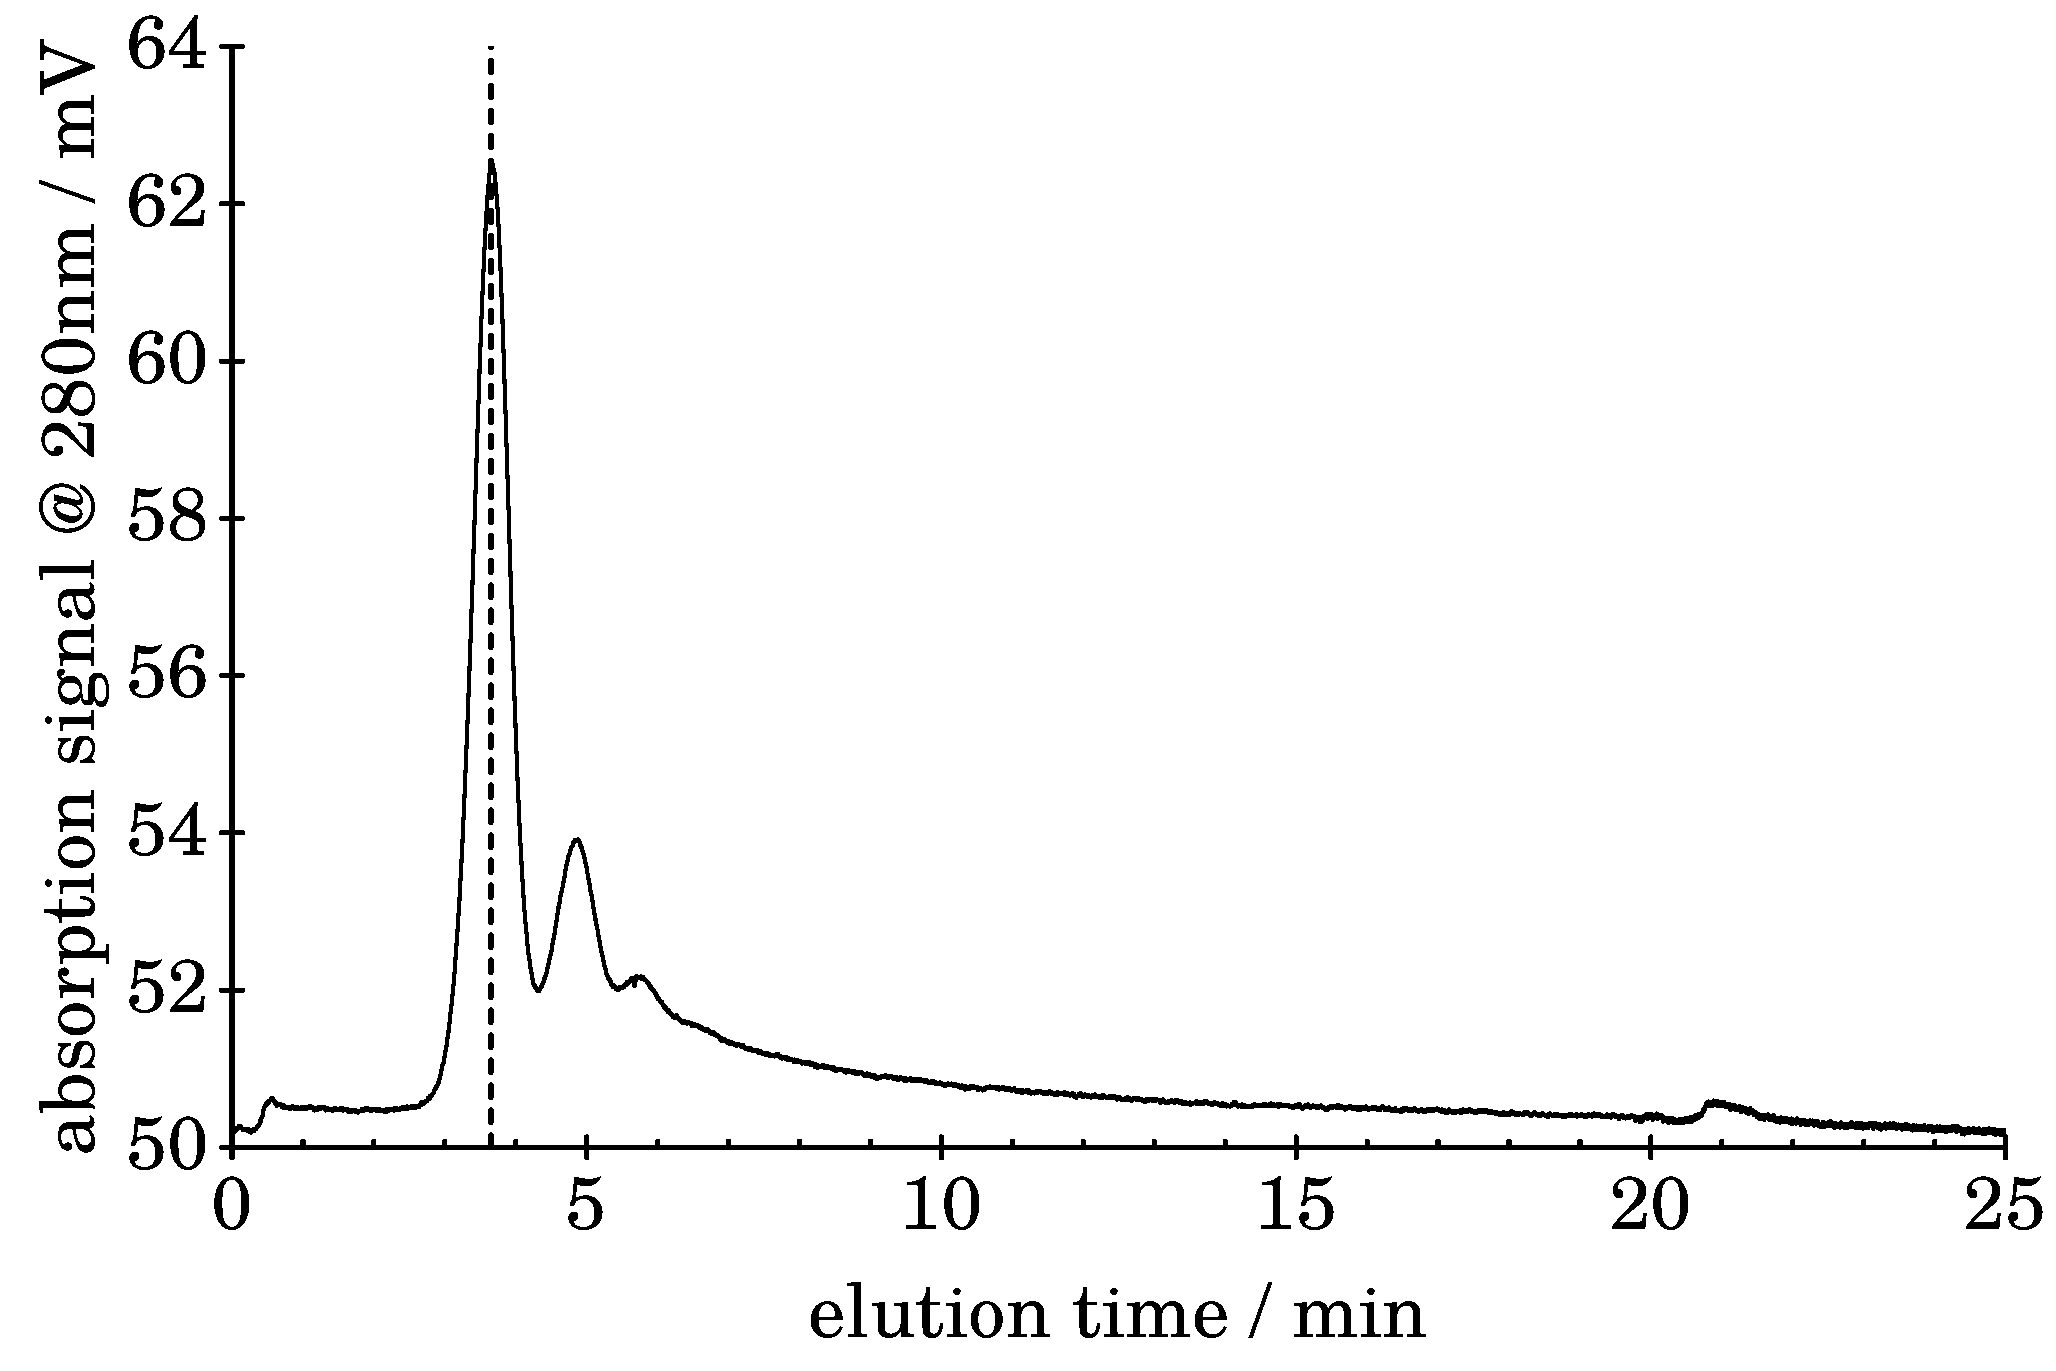
\includegraphics[width=\linewidth]{./images/data/img_BSA_VC_2_5_r2_te.pdf}
    \subcaption{Position of $\te$, replicate 2.}
    \label{subfig:raw_BSA2_5_r2_te}
  \end{subfigure}
  \begin{subfigure}{\subFigSize}
    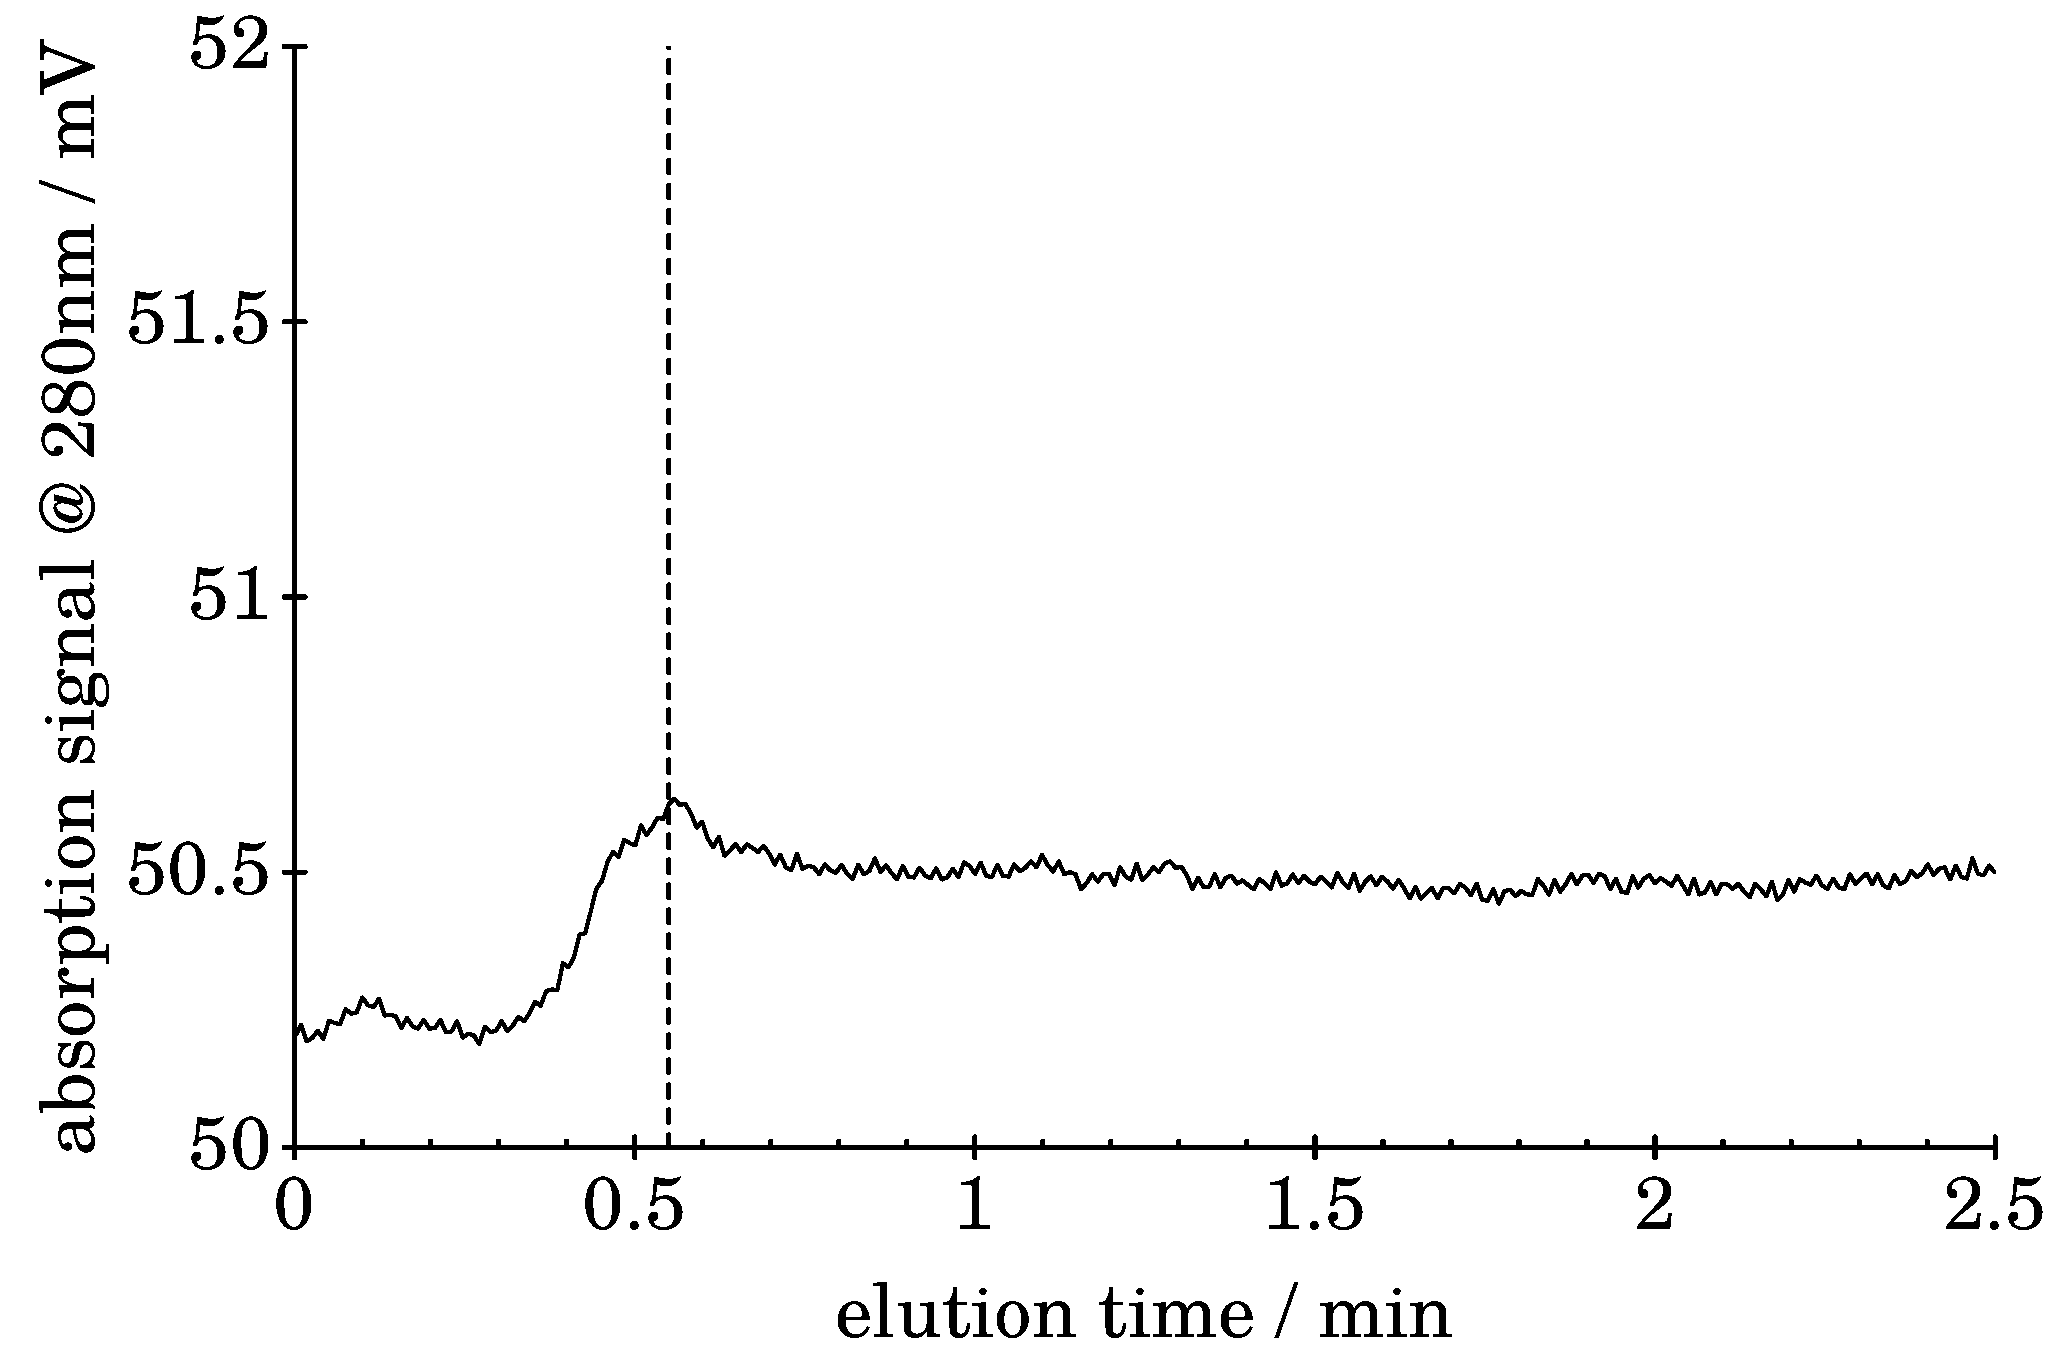
\includegraphics[width=\linewidth]{./images/data/img_BSA_VC_2_5_r2_t0.pdf}
    \subcaption{Detailed starting section of fractogram \ref{subfig:raw_BSA2_5_r2_te};
      Position of $\tvoid$, replicate 2.}
  \end{subfigure}
  \\\vspace*{.5em}
    %%%%%%%%%%%%%%%%%%%%%
  \begin{subfigure}{\subFigSize}
    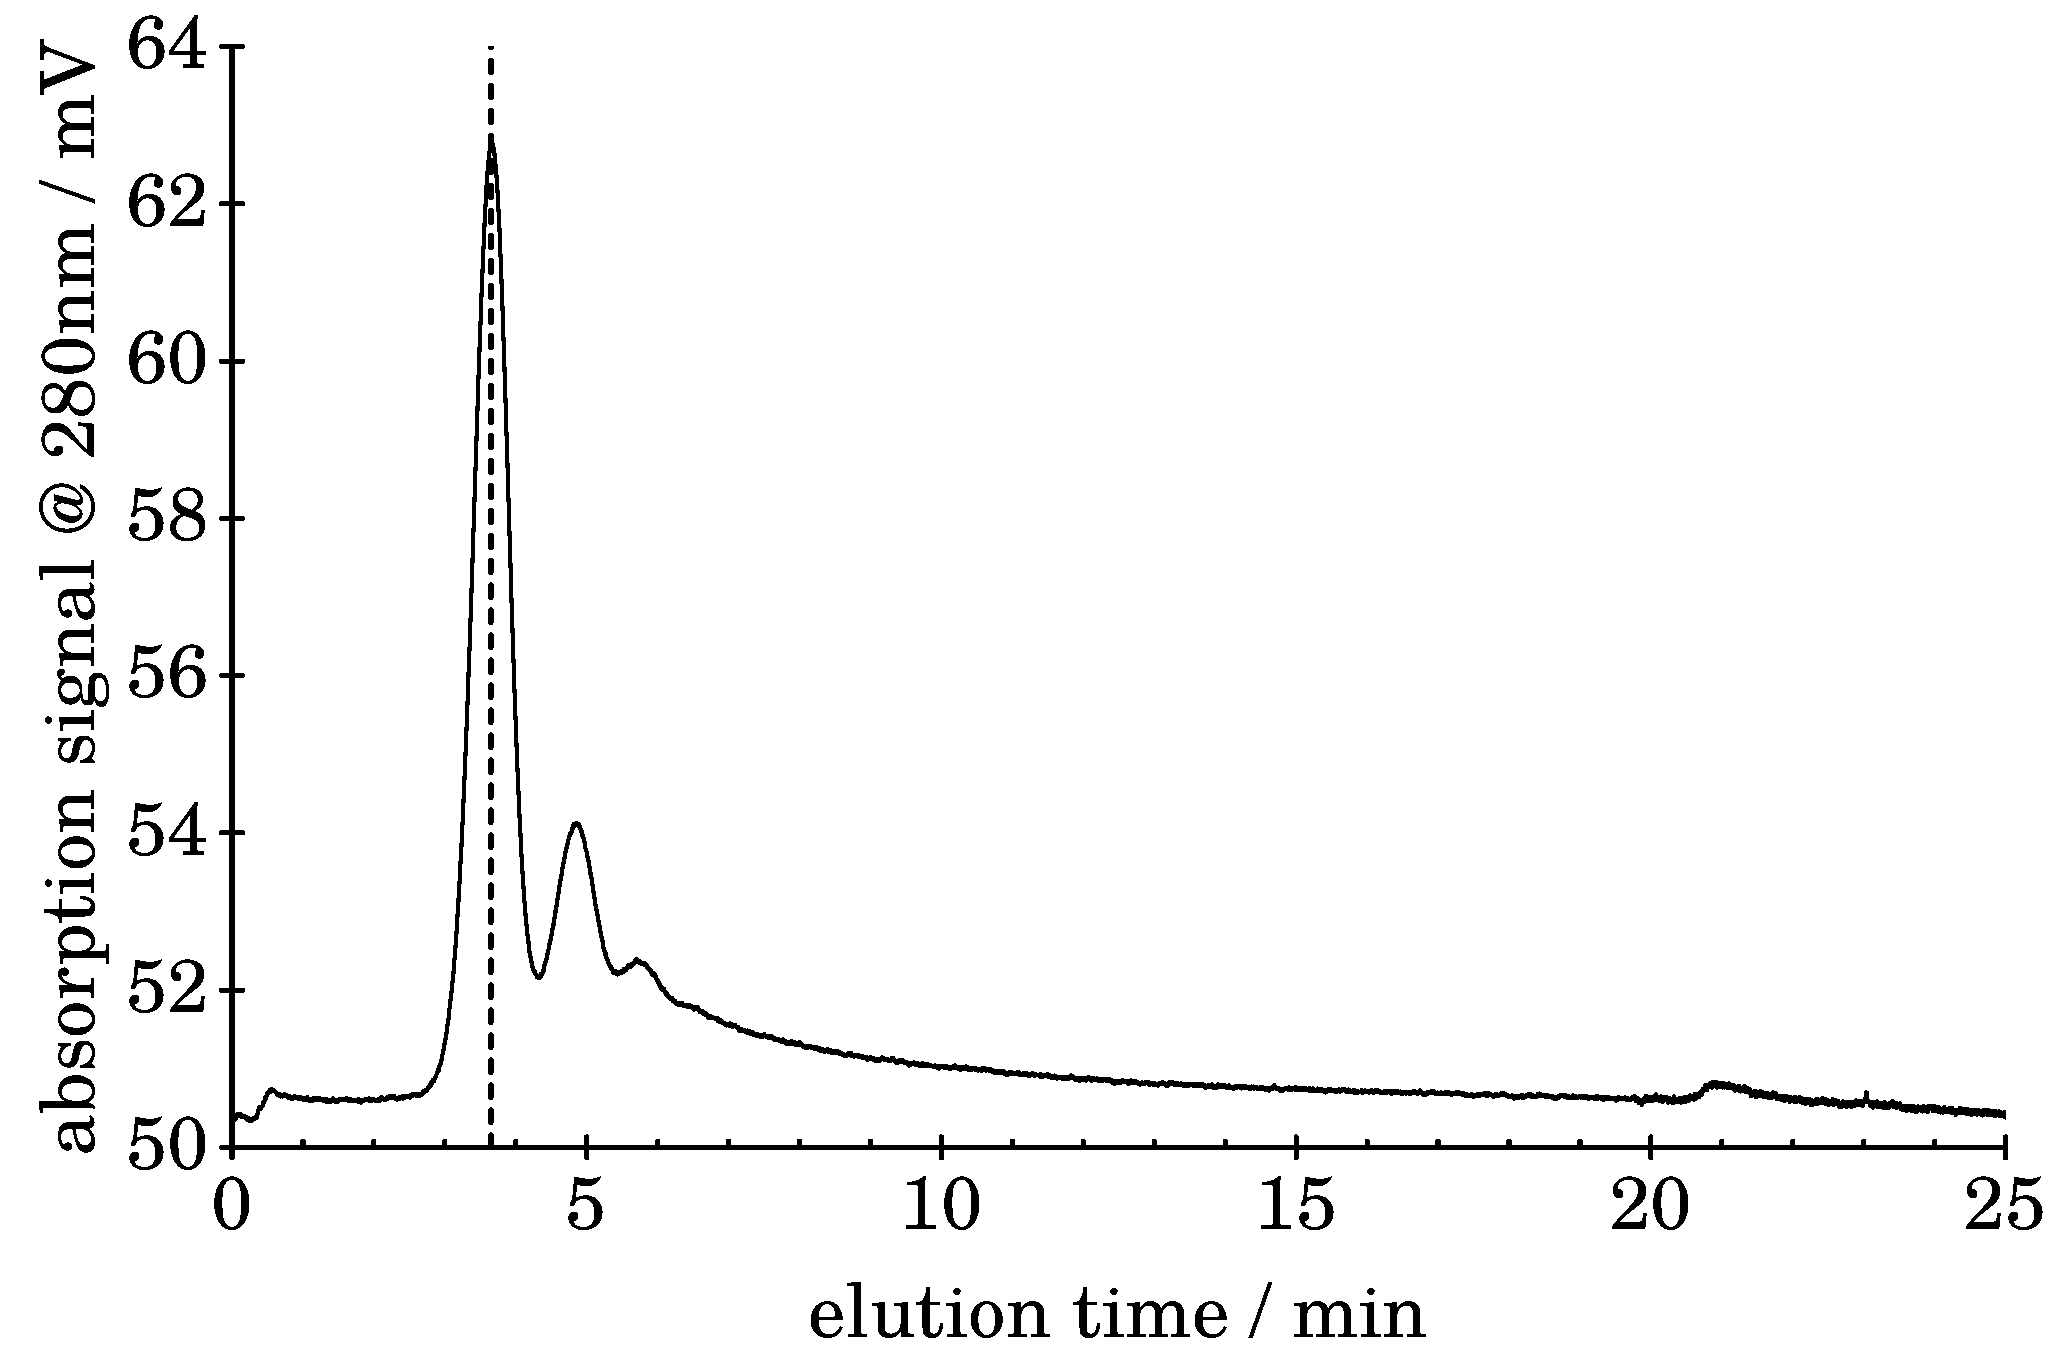
\includegraphics[width=\linewidth]{./images/data/img_BSA_VC_2_5_r3_te.pdf}
    \subcaption{Position of $\te$, replicate 3.}
    \label{subfig:raw_BSA2_5_r3_te}
  \end{subfigure}
  \begin{subfigure}{\subFigSize}
    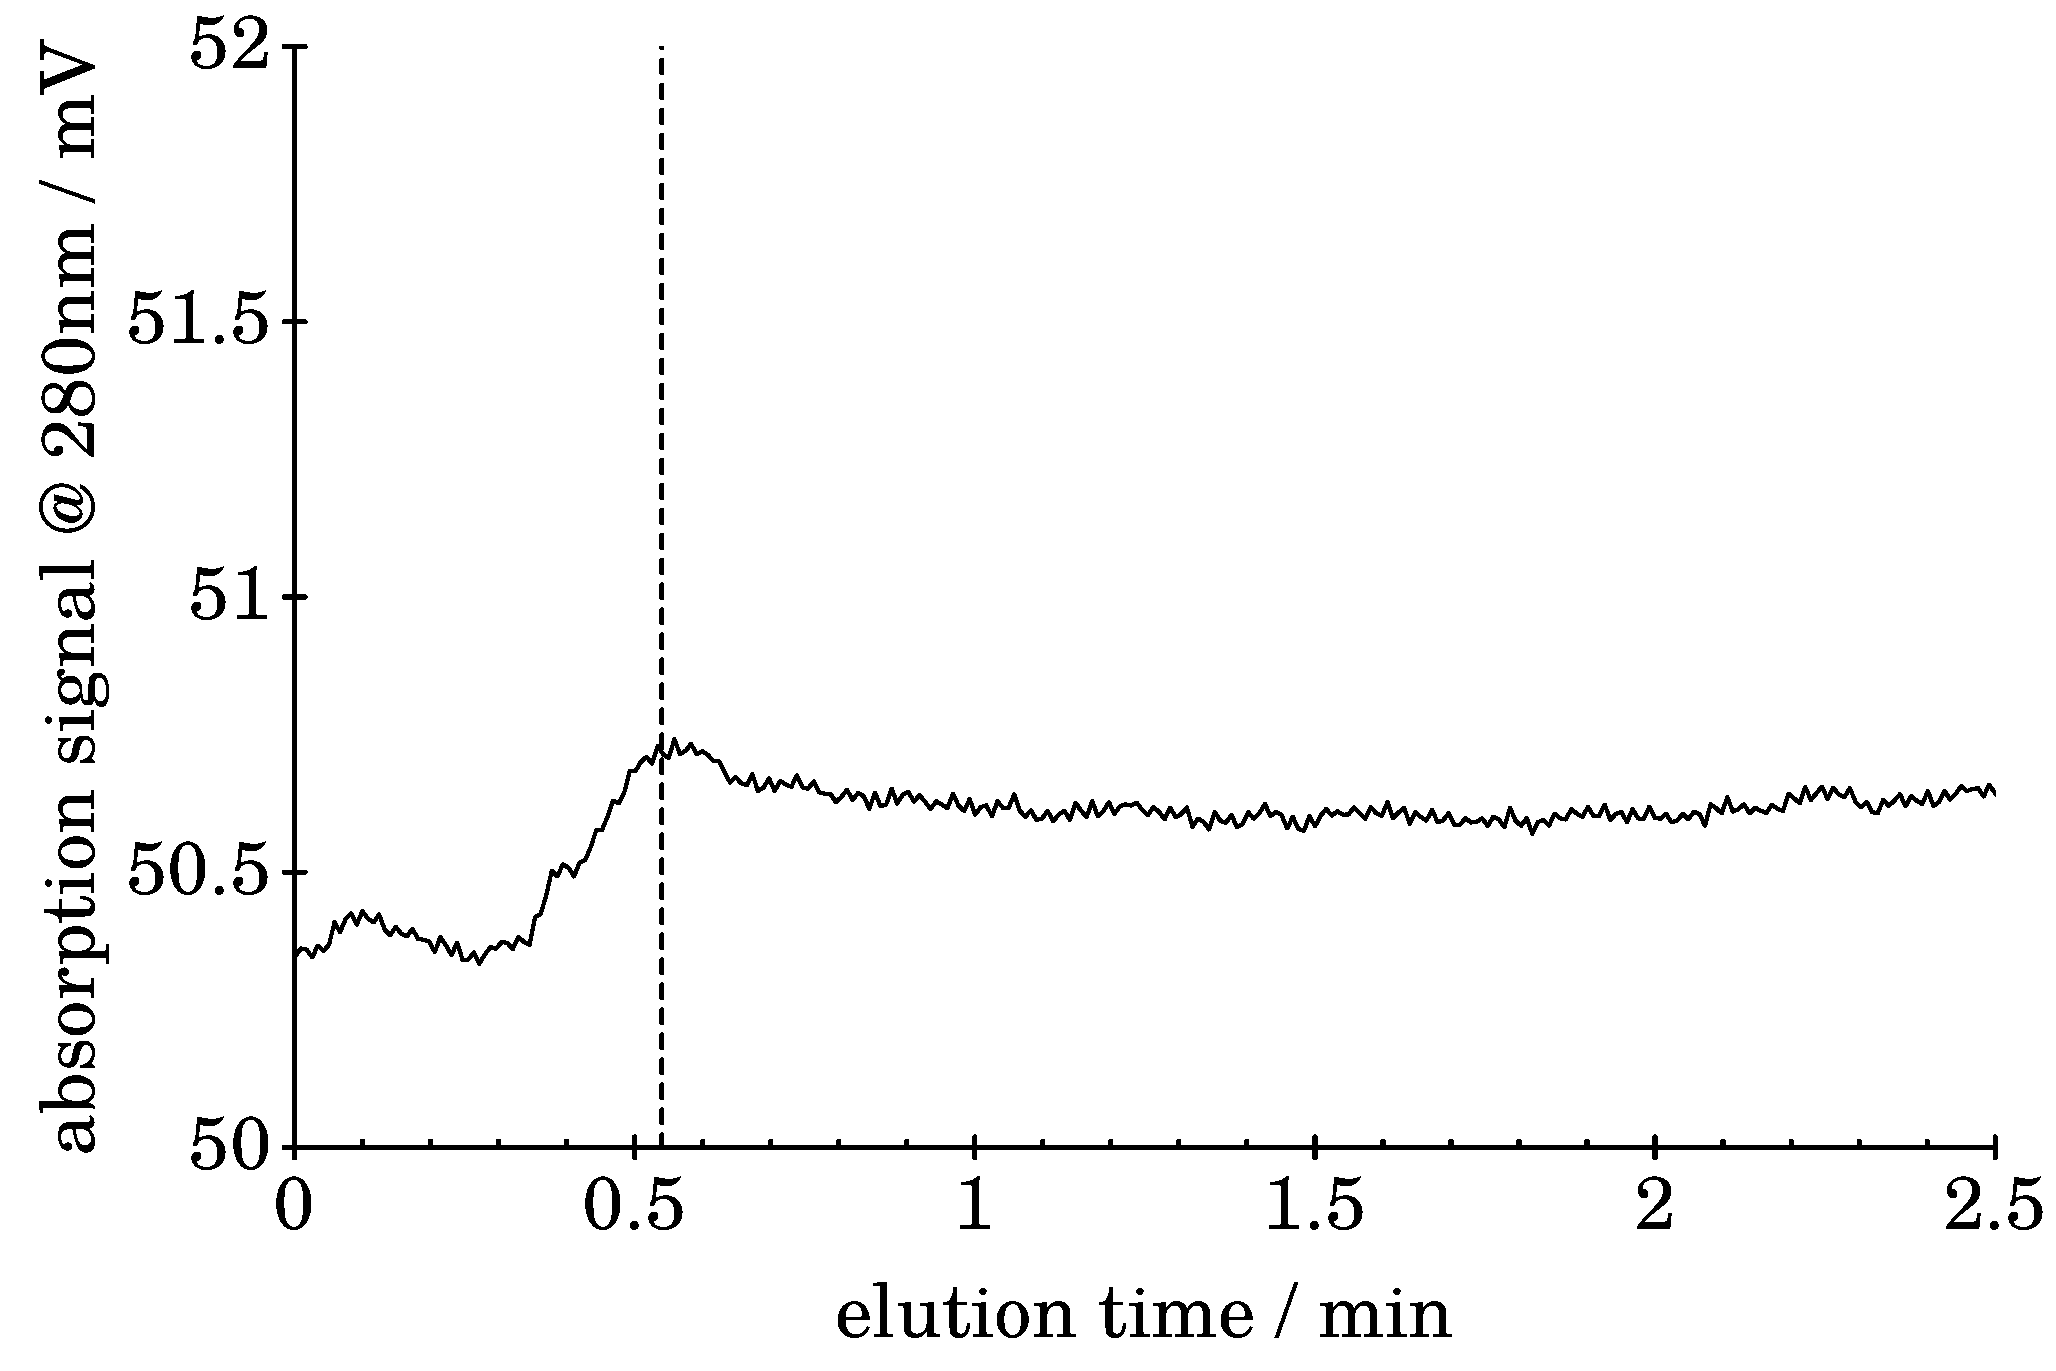
\includegraphics[width=\linewidth]{./images/data/img_BSA_VC_2_5_r3_t0.pdf}
    \subcaption{Detailed starting section of fractogram \ref{subfig:raw_BSA2_5_r3_te};
      Position of $\tvoid$, replicate 3.}
  \end{subfigure}
  \end{center}
  \vspace*{-3ex}    
  \caption[Raw fractograms of BSA measurements at $\Vc = \SI{2.5}{\mlmin}$]{Raw fractograms of BSA measurements at $\Vc 
  = \SI{2.5}{\mlmin}$}
  \label{fig:raw_BSA_2_5_UV} 
\end{figure}
\flushbottom
%%%%%%%%%%%%%%%%%%%%%%%%%%%%%%%%%%%%%%%%%%5
%%% BSA at Vc = 3.5 ml/min
%%%%%%%%%%%%%%%%%%%%%%%%%%%%%%%%%%%%%%%%
\begin{figure}[H]
  \begin{center}
    \begin{subfigure}{\subFigSize}
      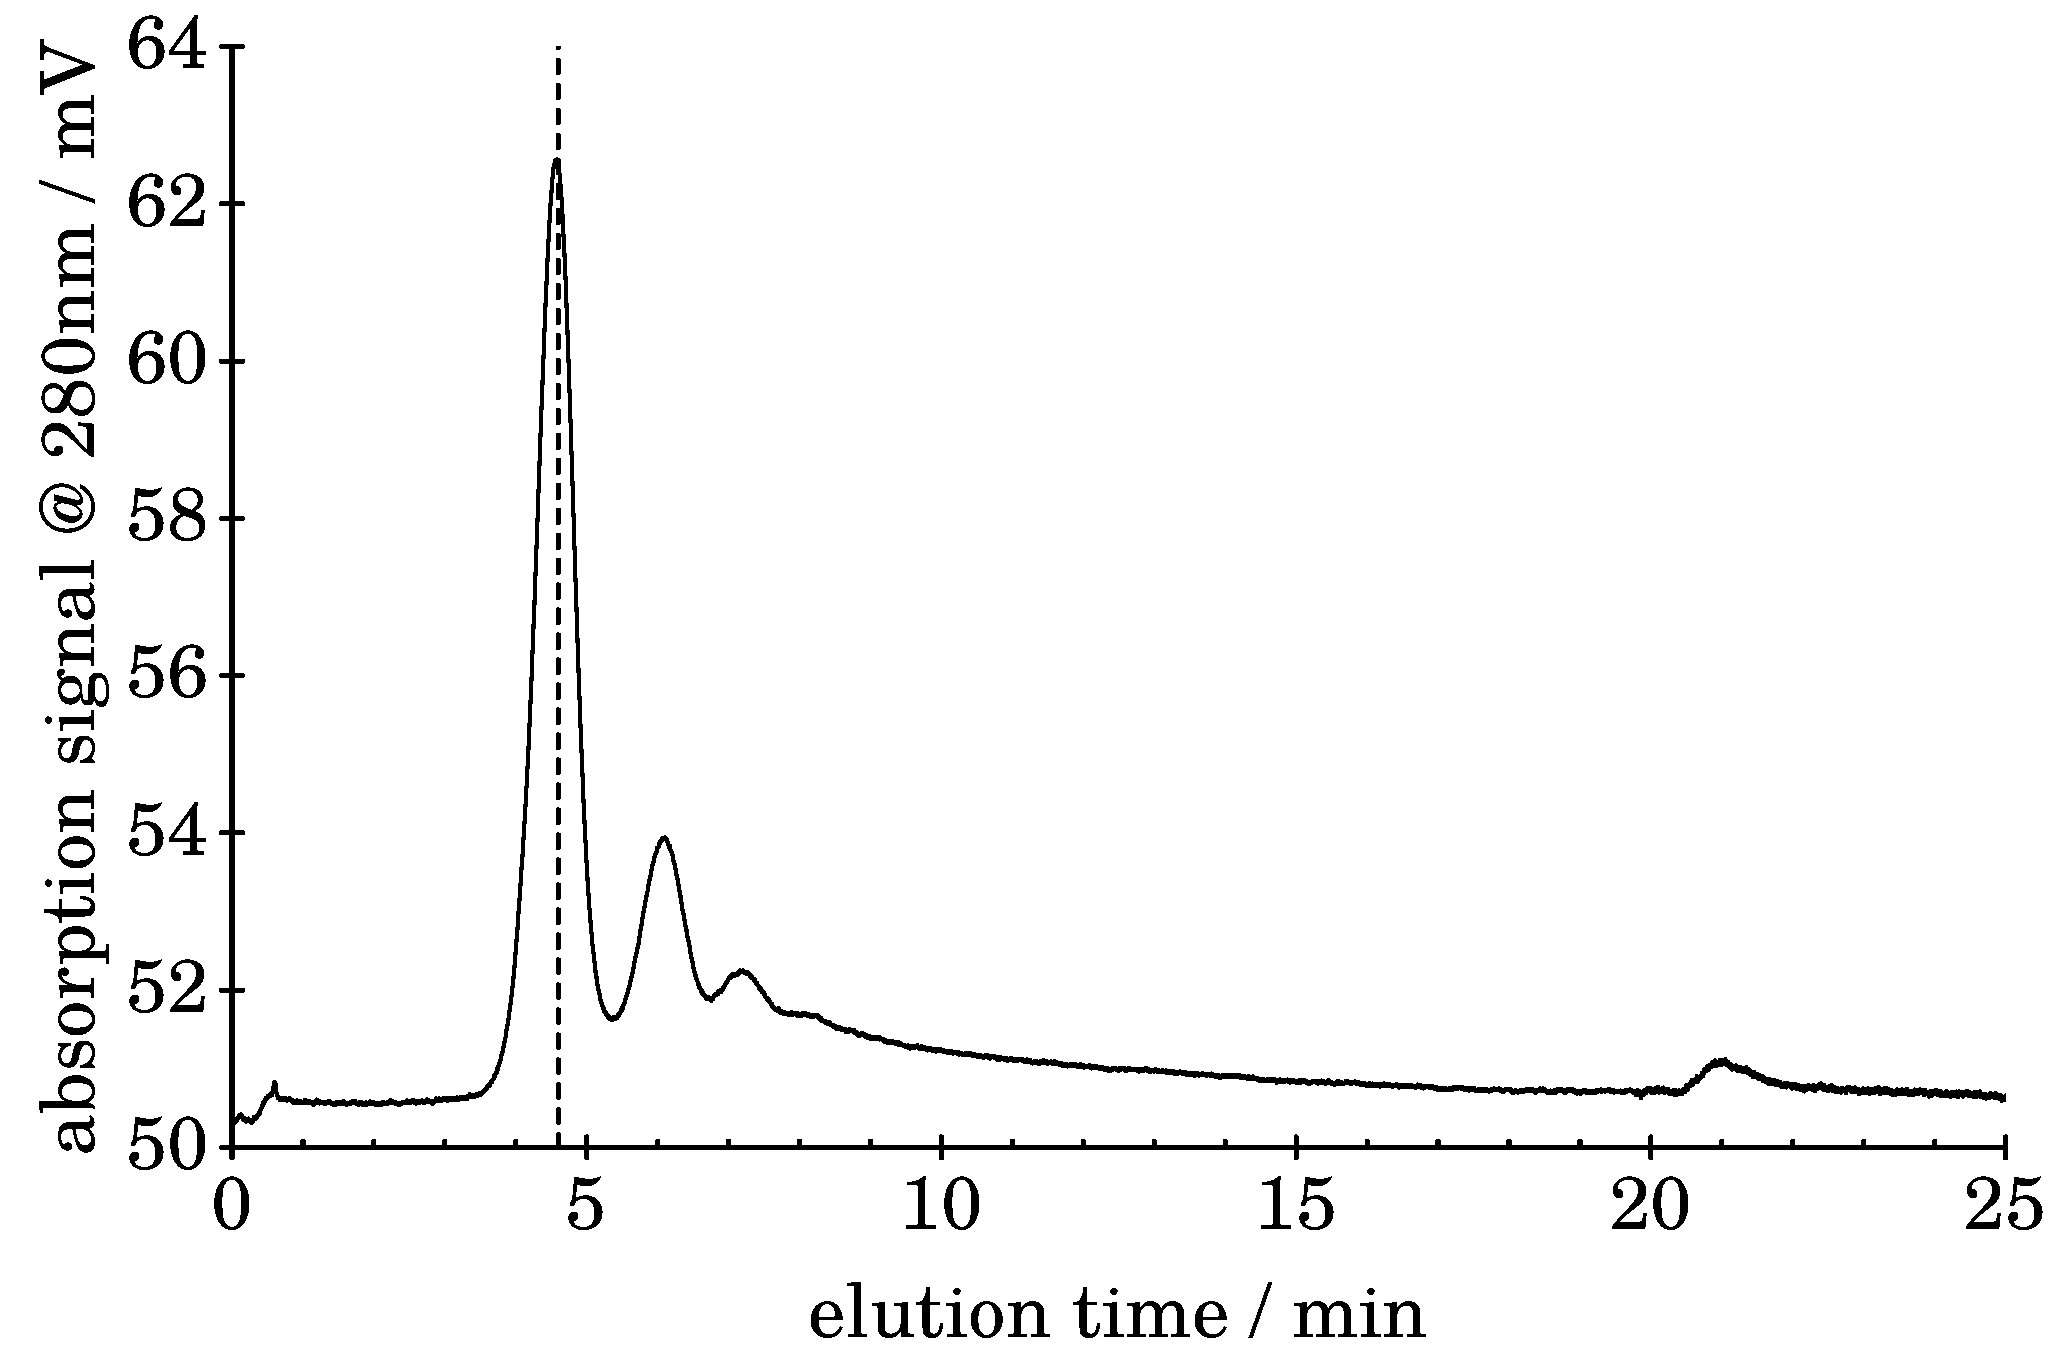
\includegraphics[width=\linewidth]{./images/data/img_BSA_VC_3_5_r1_te.pdf}
      \subcaption{Position of $\te$, replicate 1.}
      \label{subfig:raw_BSA3_5_r1_te}
    \end{subfigure}
    \begin{subfigure}{\subFigSize}
      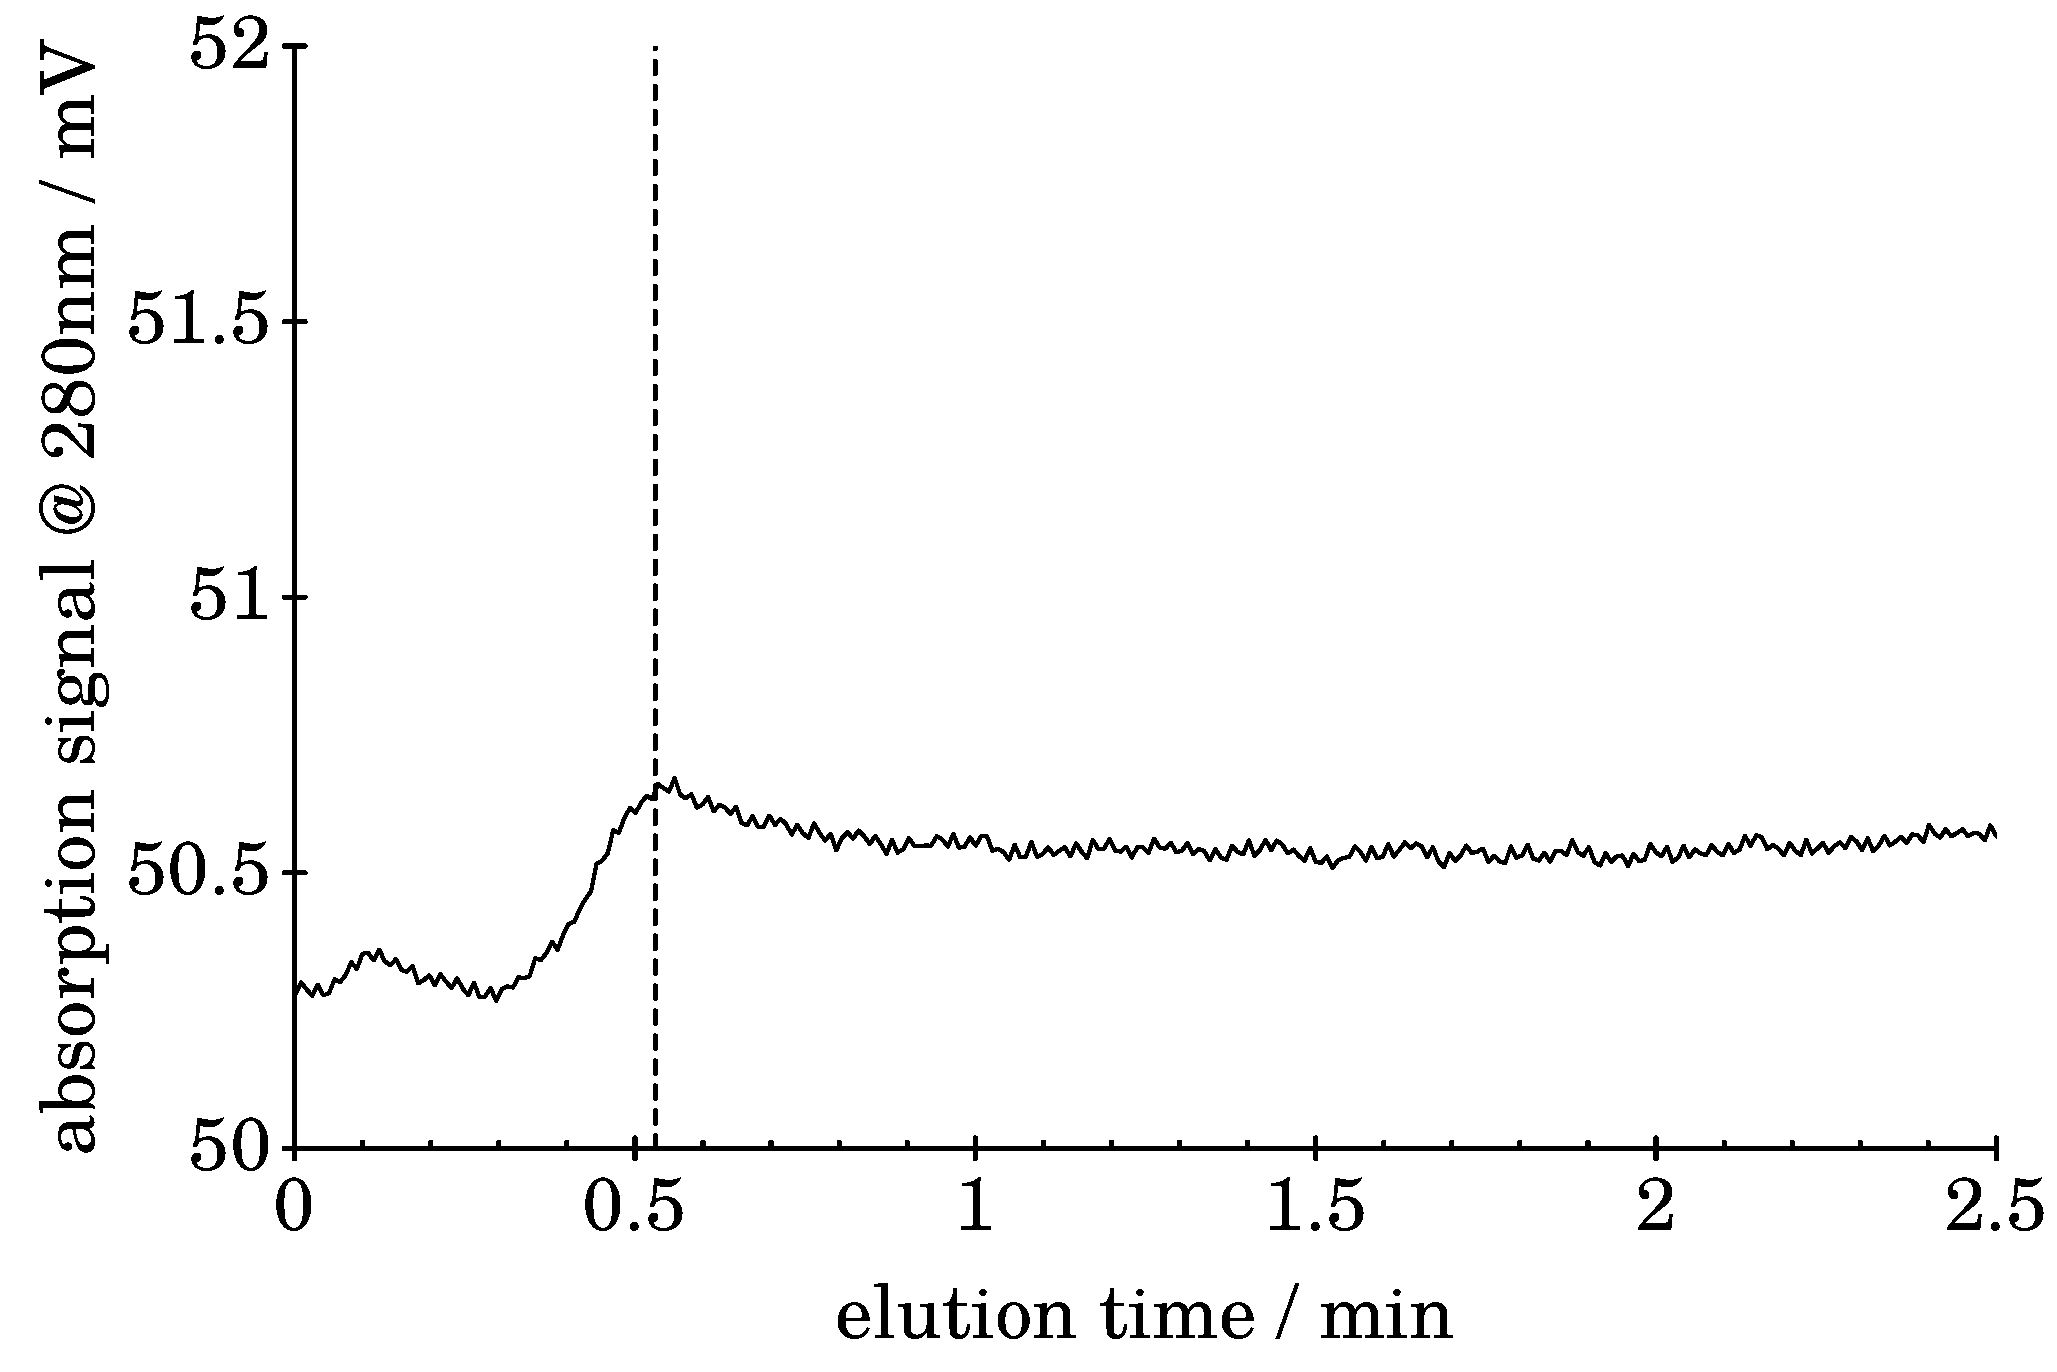
\includegraphics[width=\linewidth]{./images/data/img_BSA_VC_2_5_r1_t0.pdf}
      \subcaption{Detailed starting section of fractogram \ref{subfig:raw_BSA3_5_r1_te};
        Position of $\tvoid$, replicate 1.}
    \end{subfigure}
    \\\vspace*{.5em}
    %%%%%%%%%%%%%%%%%%%%%
    \begin{subfigure}{\subFigSize}
      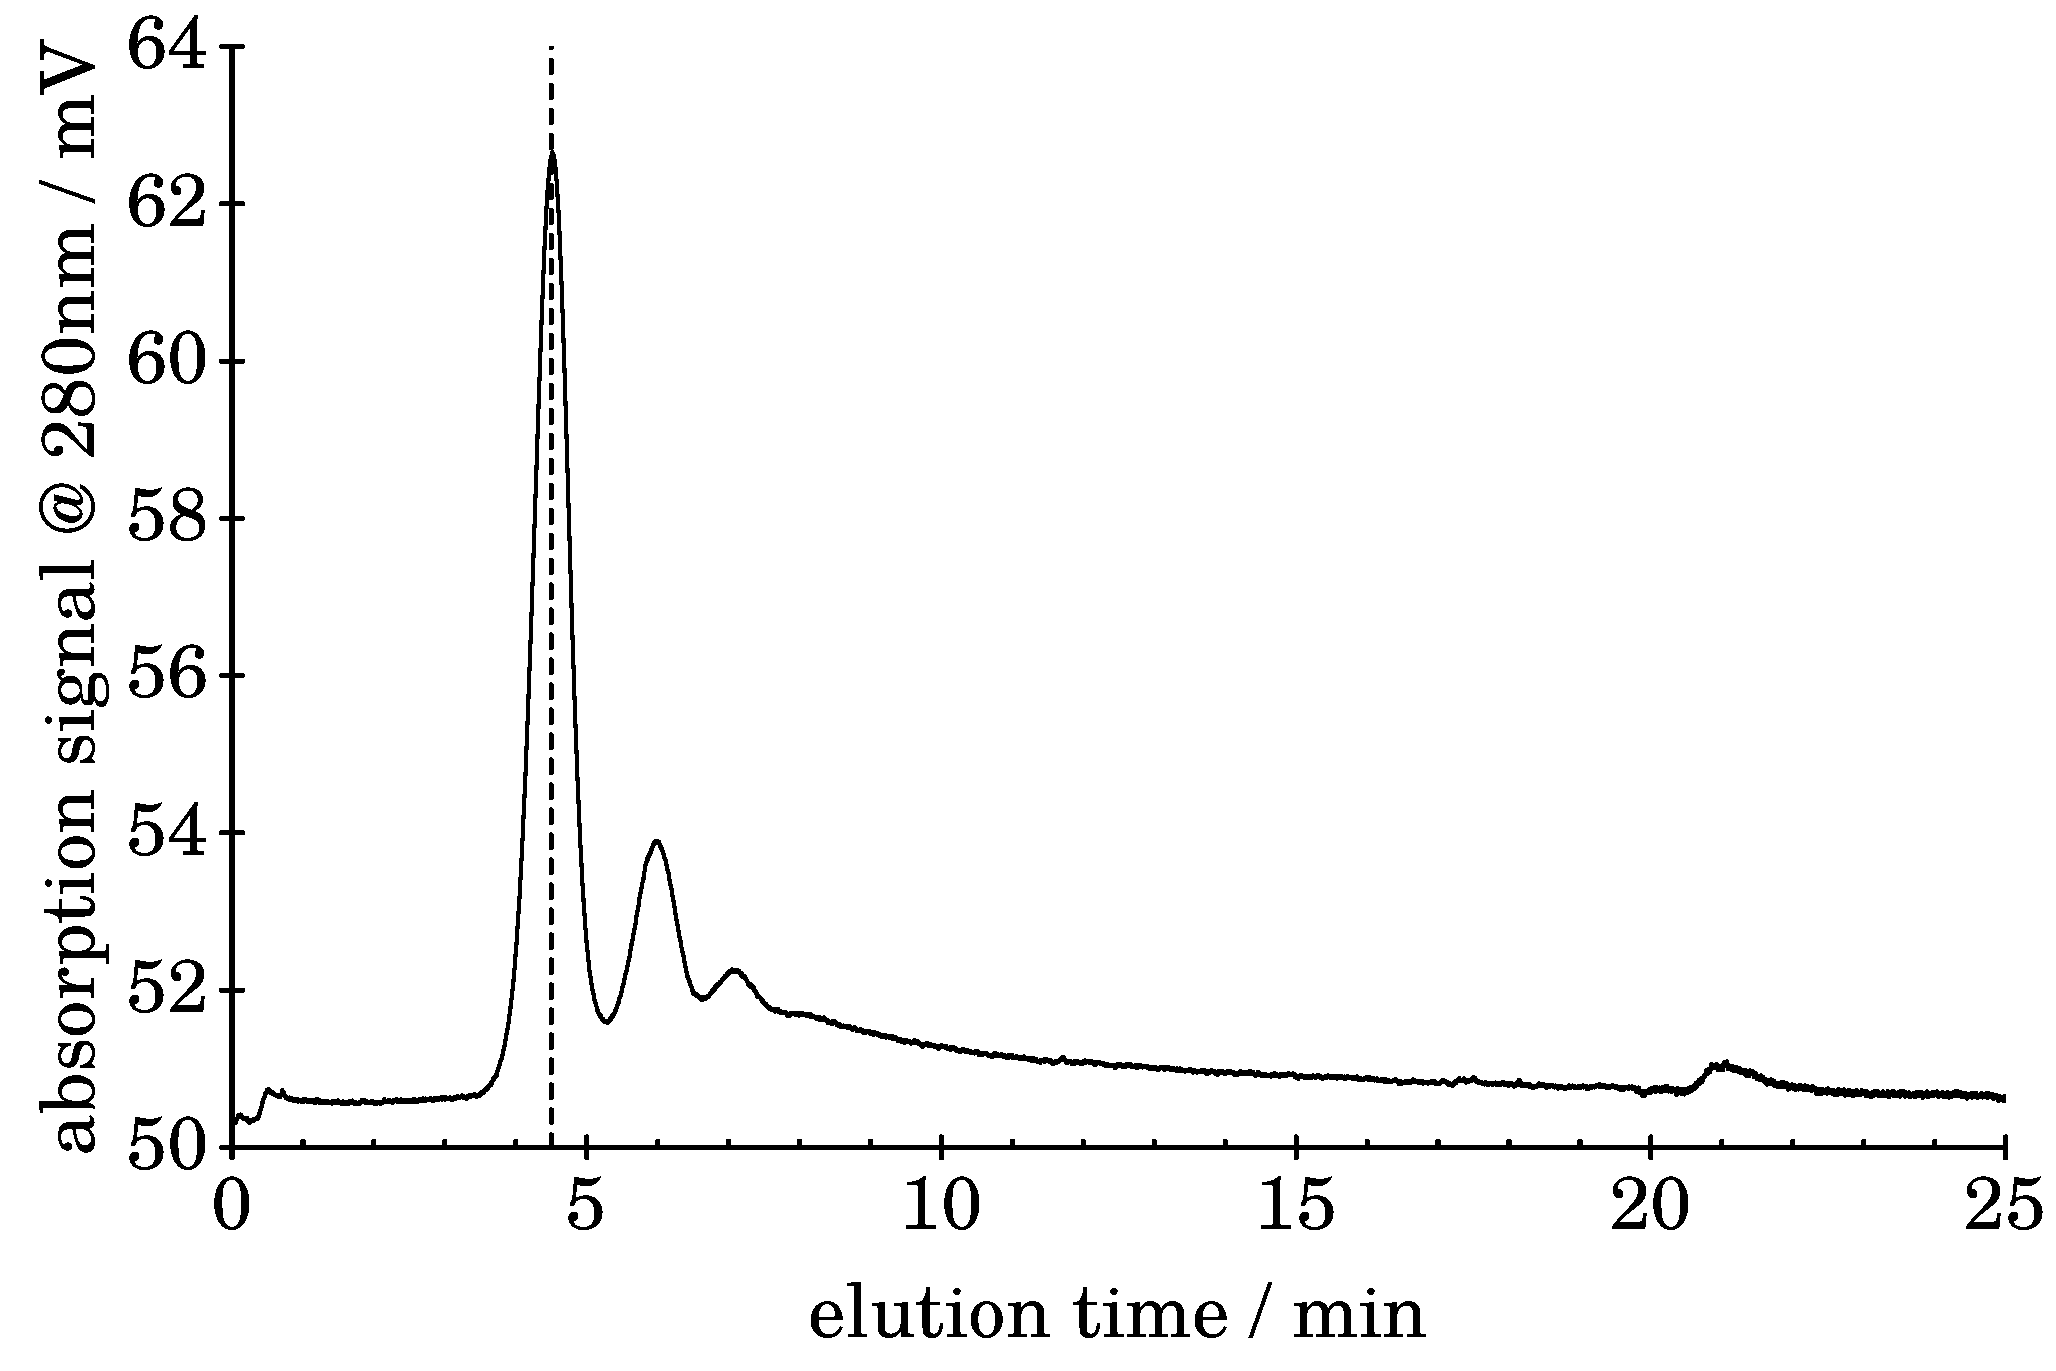
\includegraphics[width=\linewidth]{./images/data/img_BSA_VC_3_5_r2_te.pdf}
      \subcaption{Position of $\te$, replicate 2.}
      \label{subfig:raw_BSA3_5_r2_te}
    \end{subfigure}
    \begin{subfigure}{\subFigSize}
      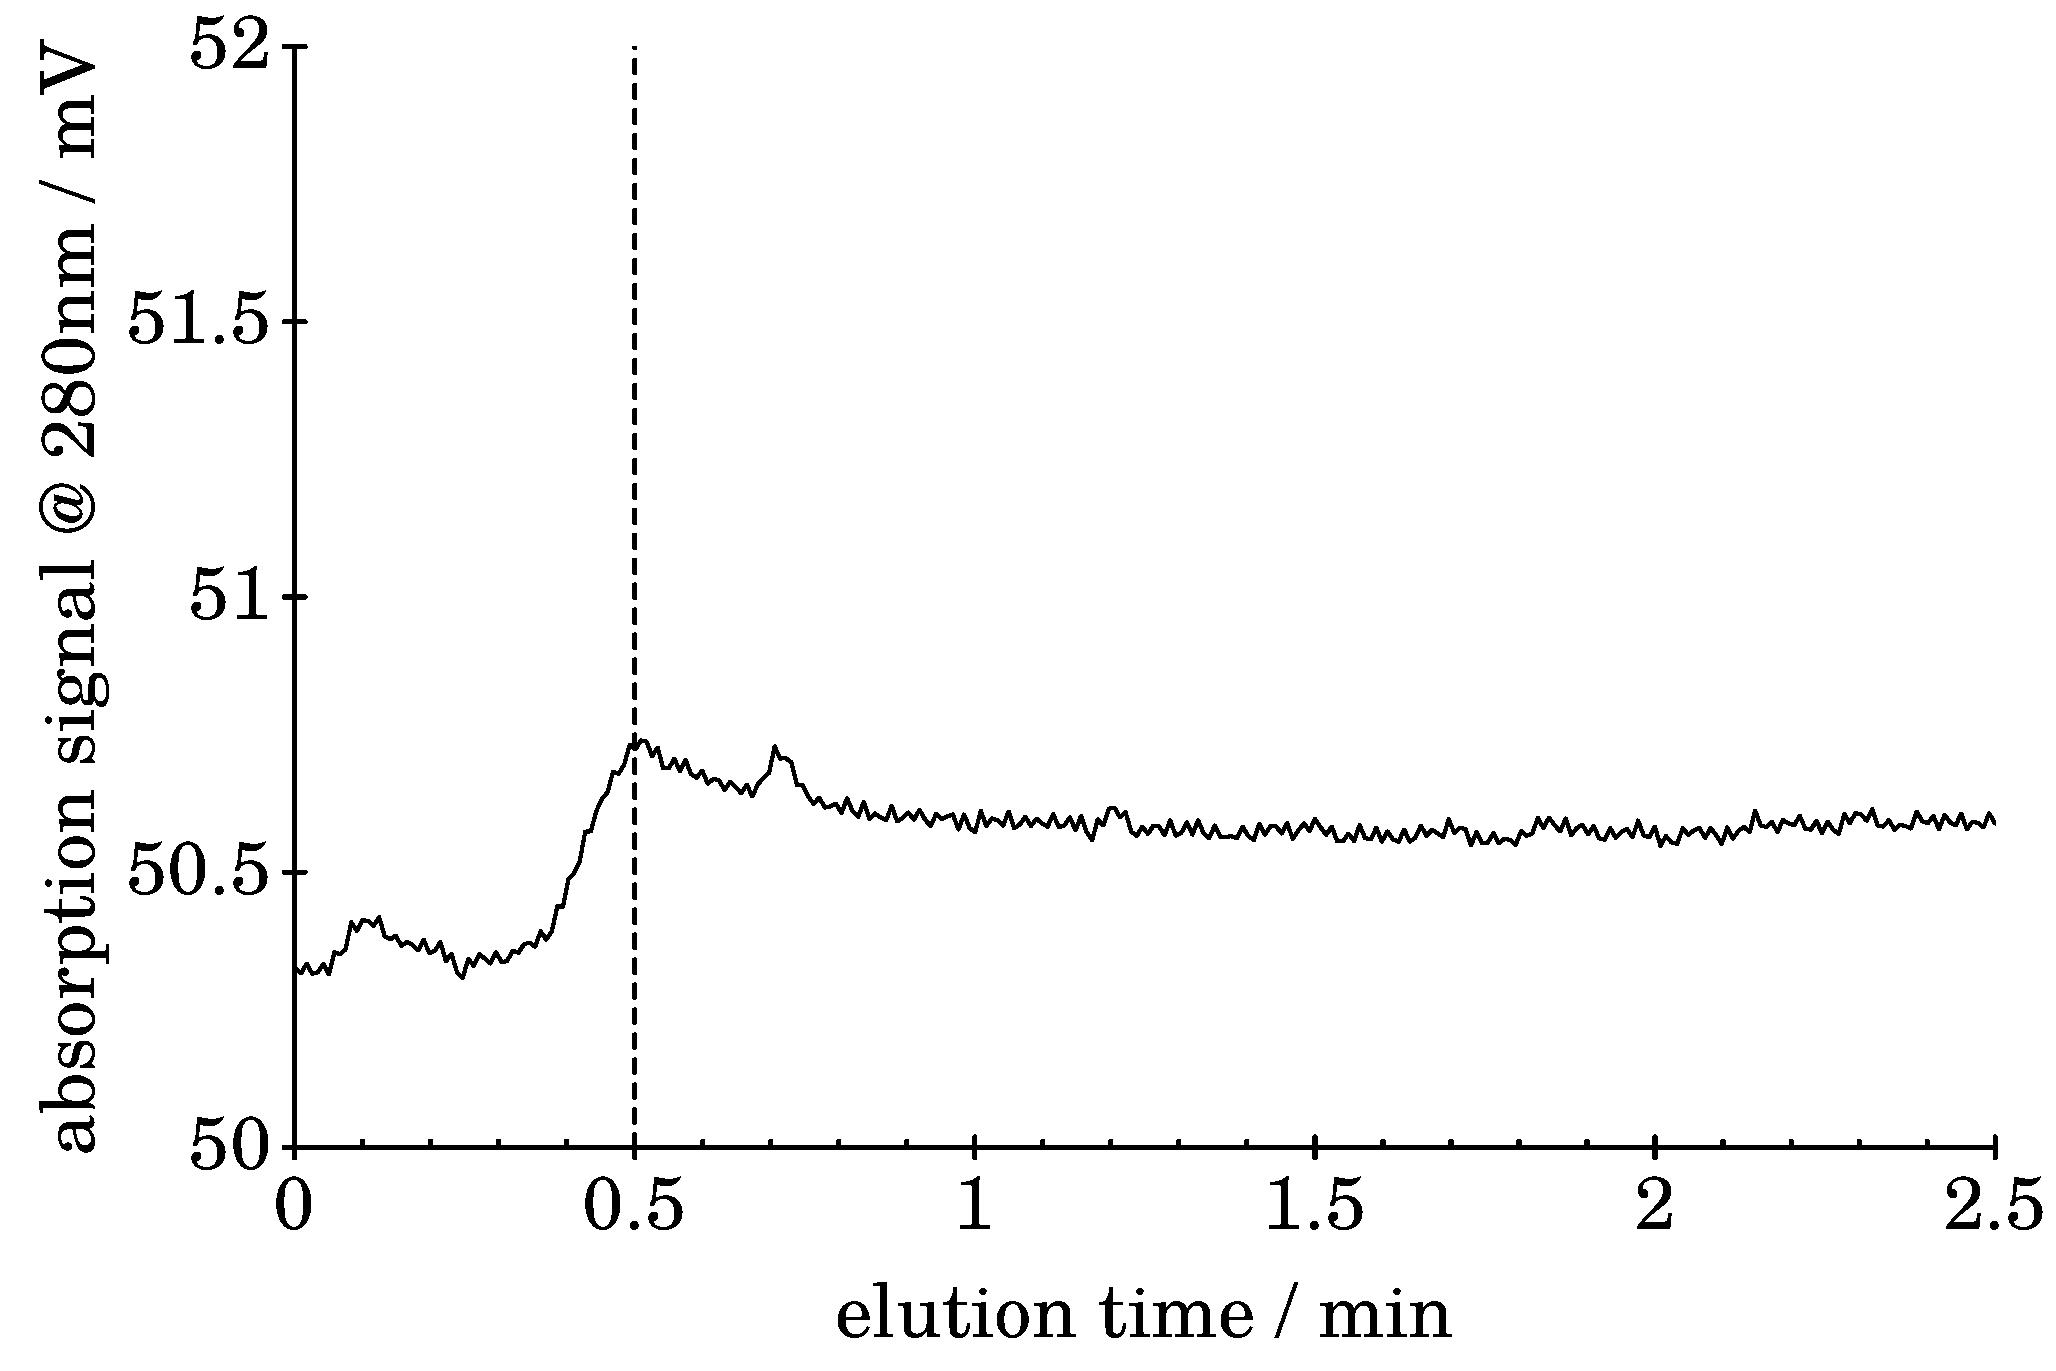
\includegraphics[width=\linewidth]{./images/data/img_BSA_VC_3_5_r2_t0.pdf}
      \subcaption{Detailed starting section of fractogram \ref{subfig:raw_BSA3_5_r2_te};
        Position of $\tvoid$, replicate 2.}
    \end{subfigure}
    \\\vspace*{.5em}
    %%%%%%%%%%%%%%%%%%%%%
    \begin{subfigure}{\subFigSize}
      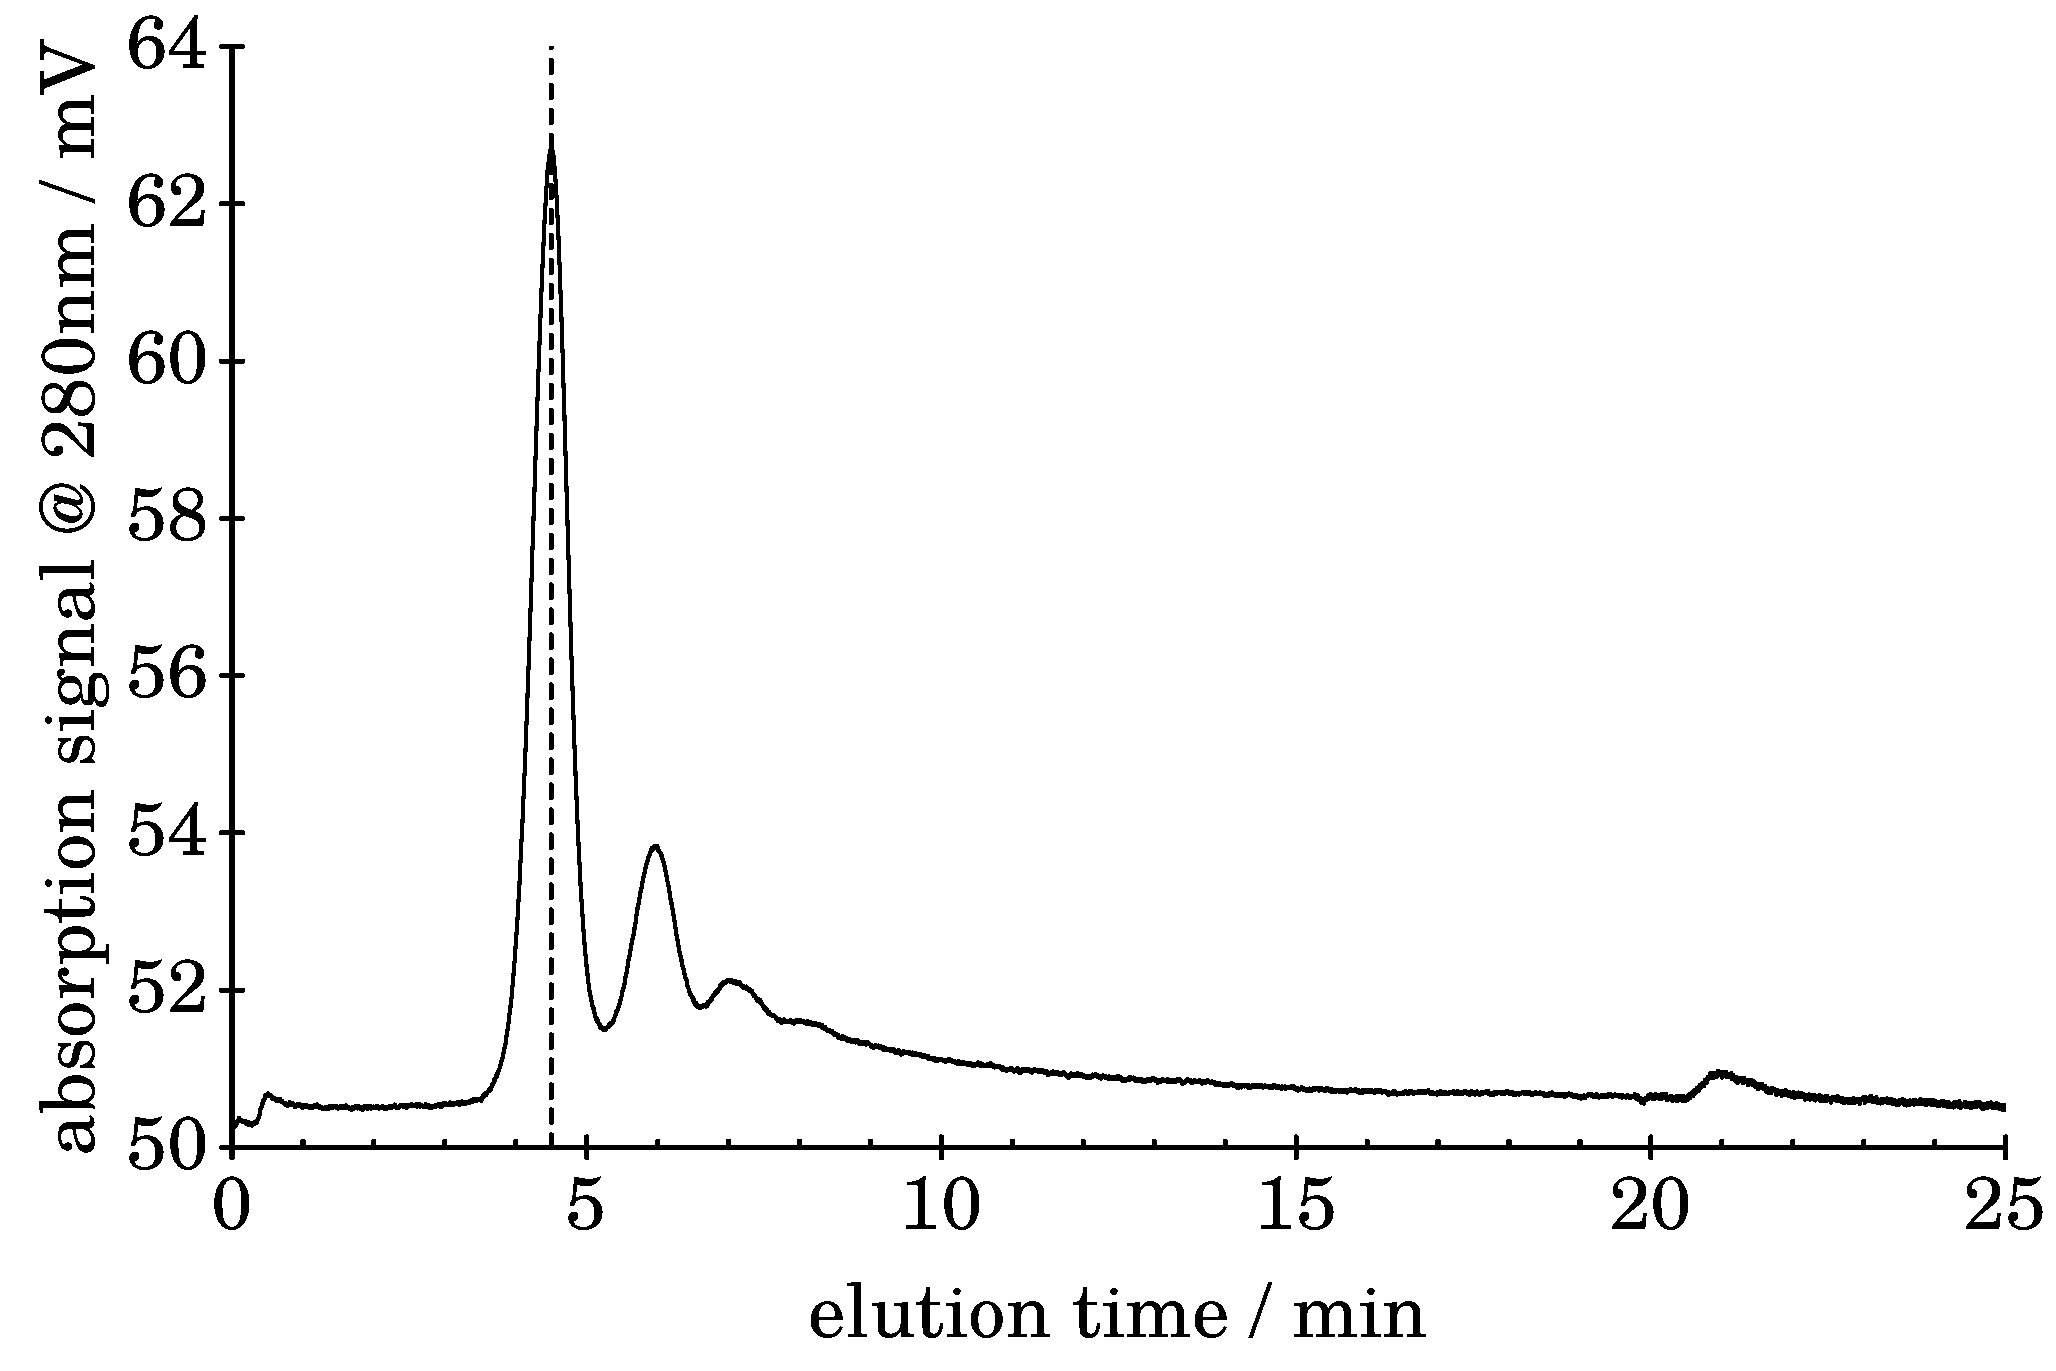
\includegraphics[width=\linewidth]{./images/data/img_BSA_VC_3_5_r3_te.pdf}
      \subcaption{Position of $\te$, replicate 3.}
      \label{subfig:raw_BSA3_5_r3_te}
    \end{subfigure}
    \begin{subfigure}{\subFigSize}
      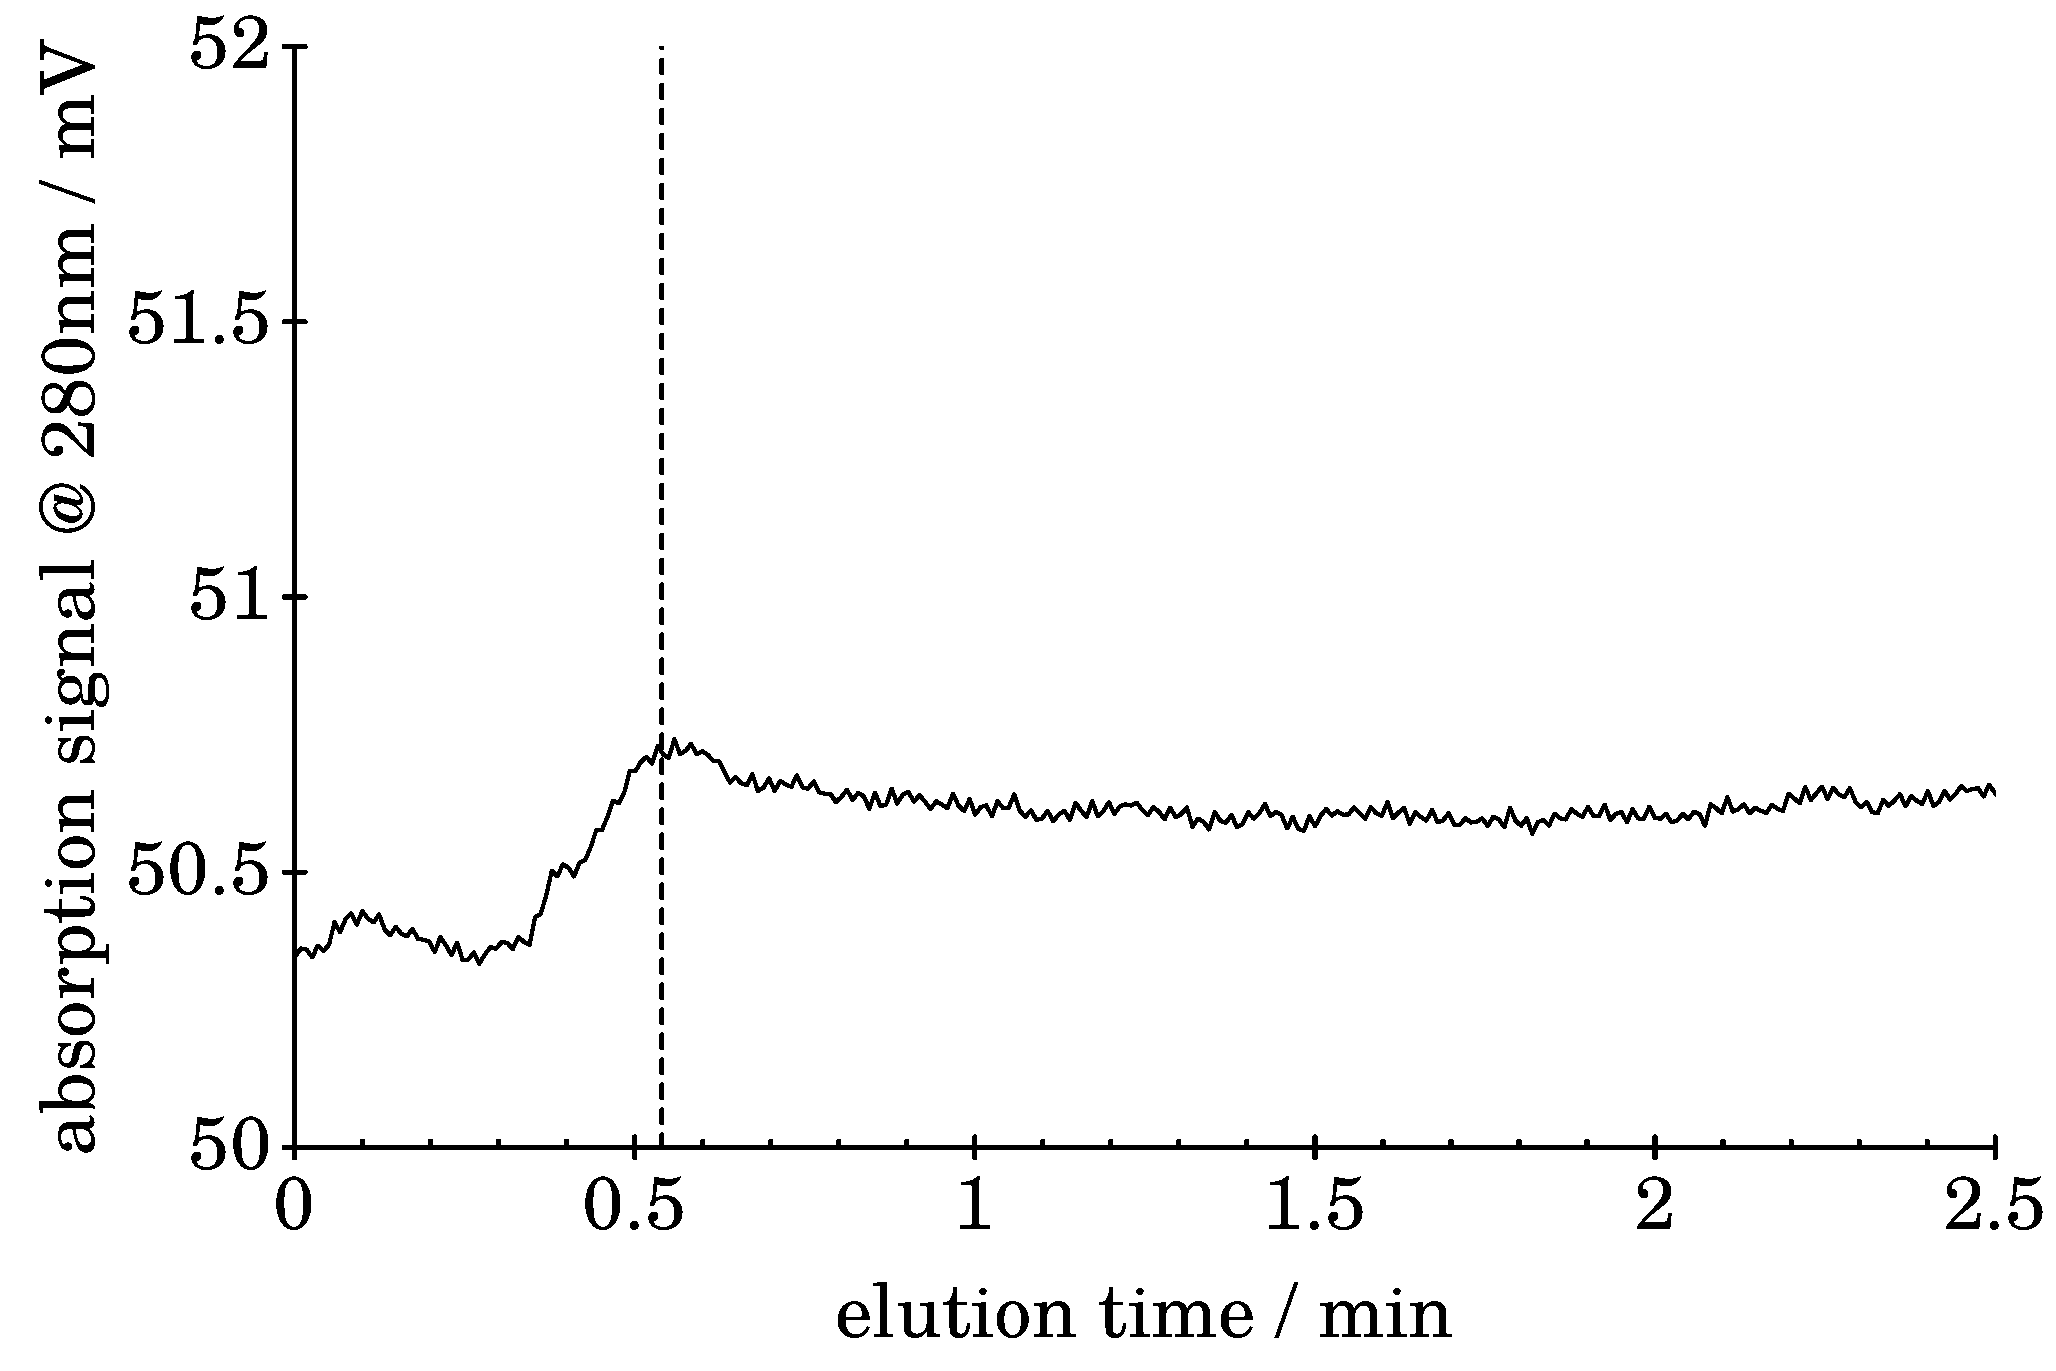
\includegraphics[width=\linewidth]{./images/data/img_BSA_VC_2_5_r3_t0.pdf}
      \subcaption{Detailed starting section of fractogram \ref{subfig:raw_BSA3_5_r3_te};
        Position of $\tvoid$, replicate 3.}
    \end{subfigure}
  \end{center}
  \vspace*{-3ex}    
  \caption[Raw fractograms of BSA measurements at $\Vc = \SI{3.5}{\mlmin}$]{Raw fractograms of BSA measurements at $\Vc 
  = \SI{3.5}{\mlmin}$}
  \label{fig:raw_BSA_3_5_UV} 
\end{figure}
\flushbottom
%%%%%%%%%%%%%%%%%%%%%%%%%%%%%%%%%%%%%%%%%%5
%%% PS at Vc = 0.5 ml/min, replicate 1
%%%%%%%%%%%%%%%%%%%%%%%%%%%%%%%%%%%%%%%%
\begin{figure}[t!]
  \begin{center}
    \begin{subfigure}{\subFigSize}
      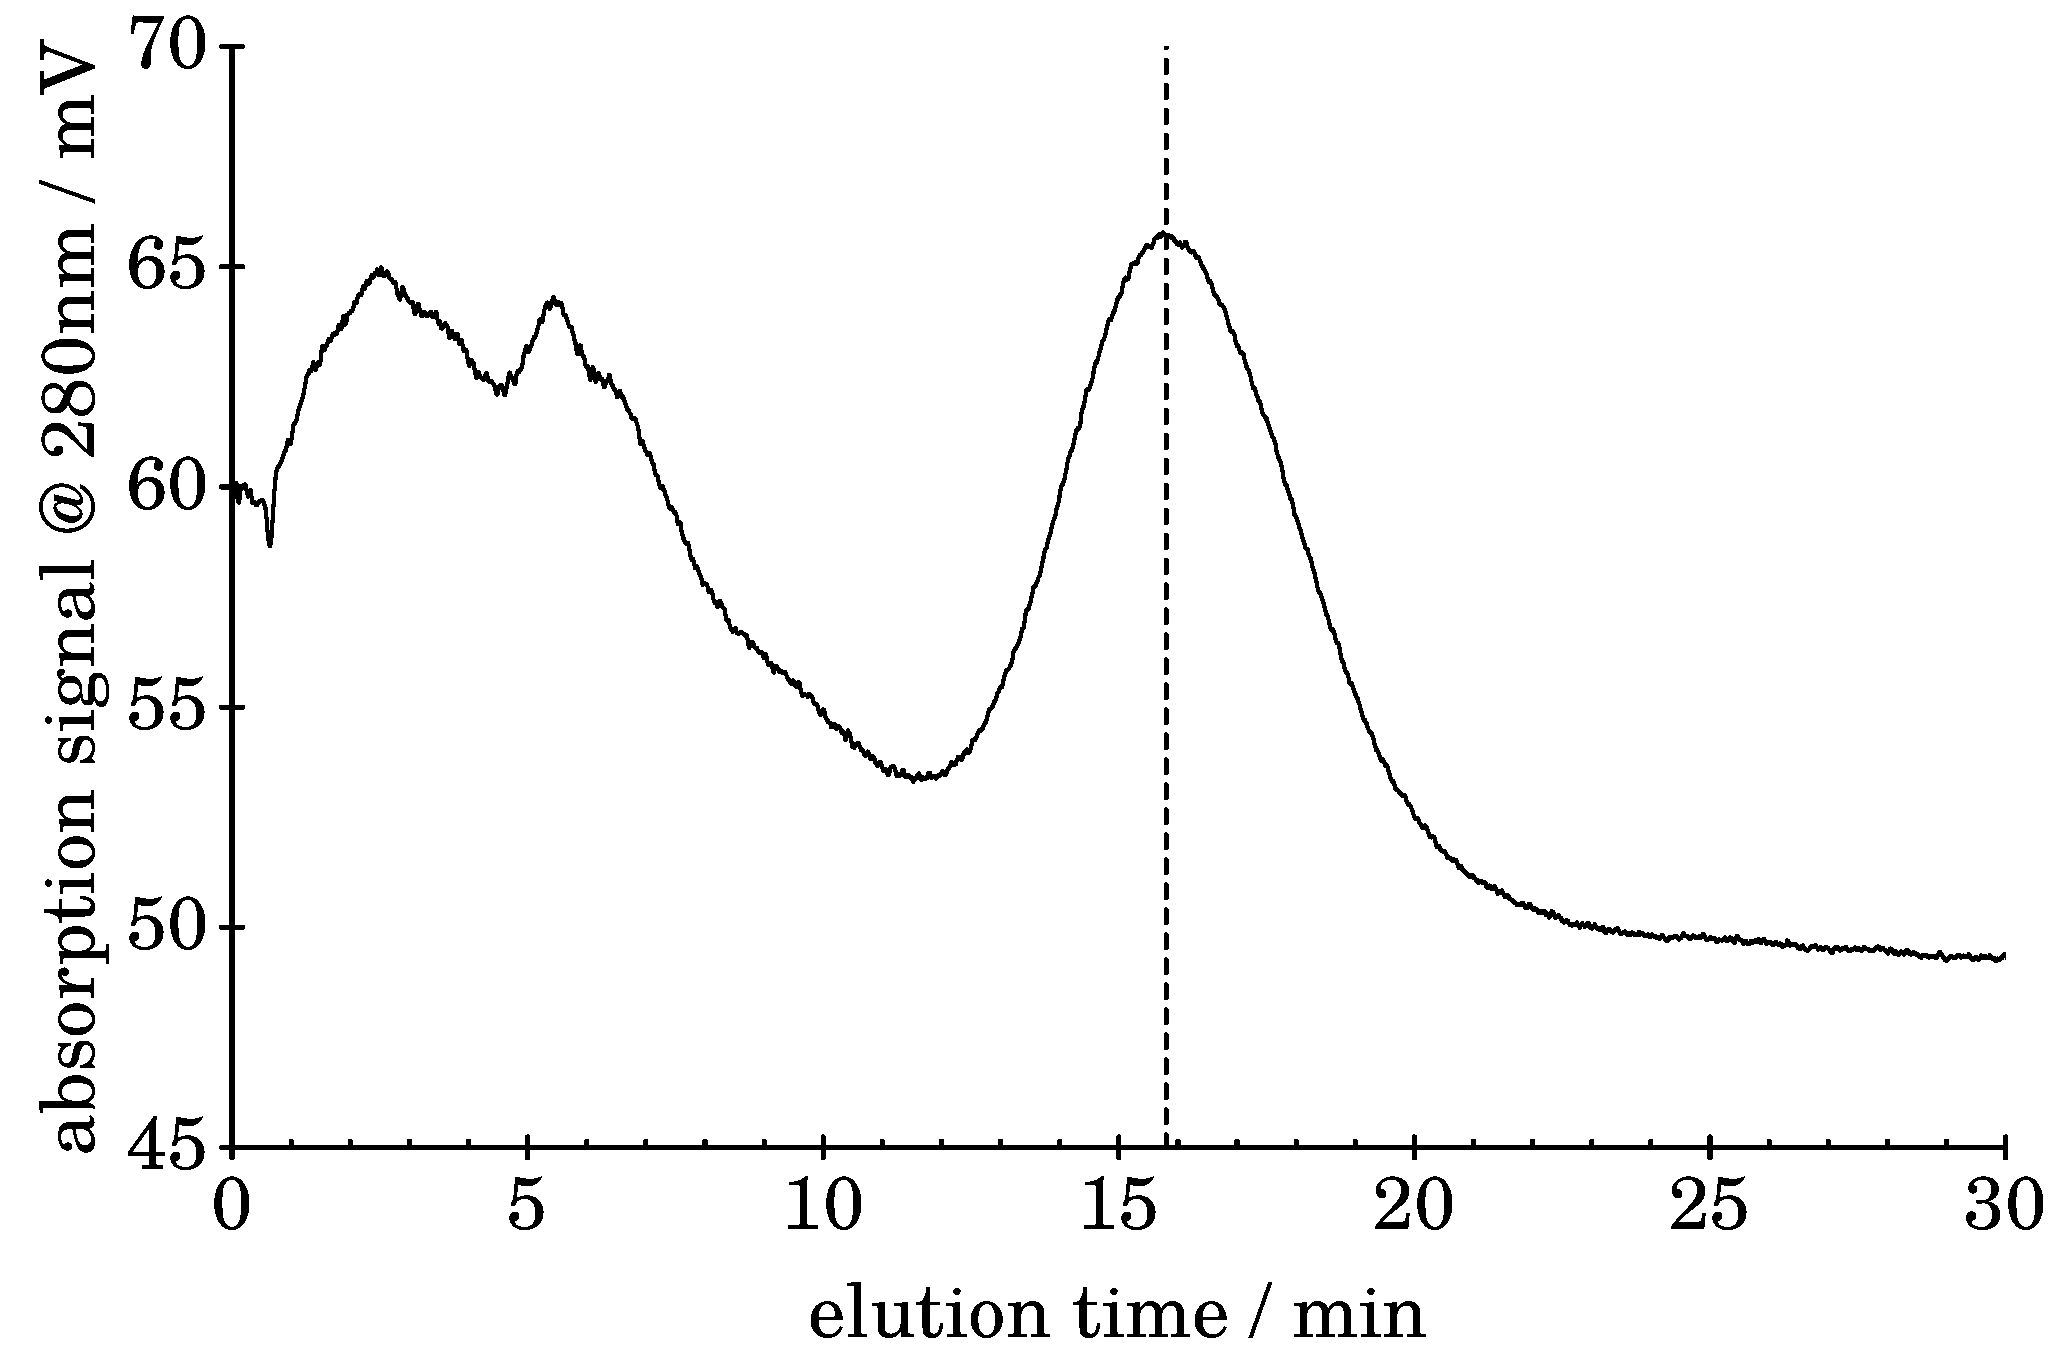
\includegraphics[width=\linewidth]{./images/data/img_PS_VC_05_rep1_te_UV.pdf}
      \subcaption{Position of $\te$ with UV detection signal}
      \label{subfig:raw_PS2_5_r1_te_UV}
    \end{subfigure}
    \begin{subfigure}{\subFigSize}
      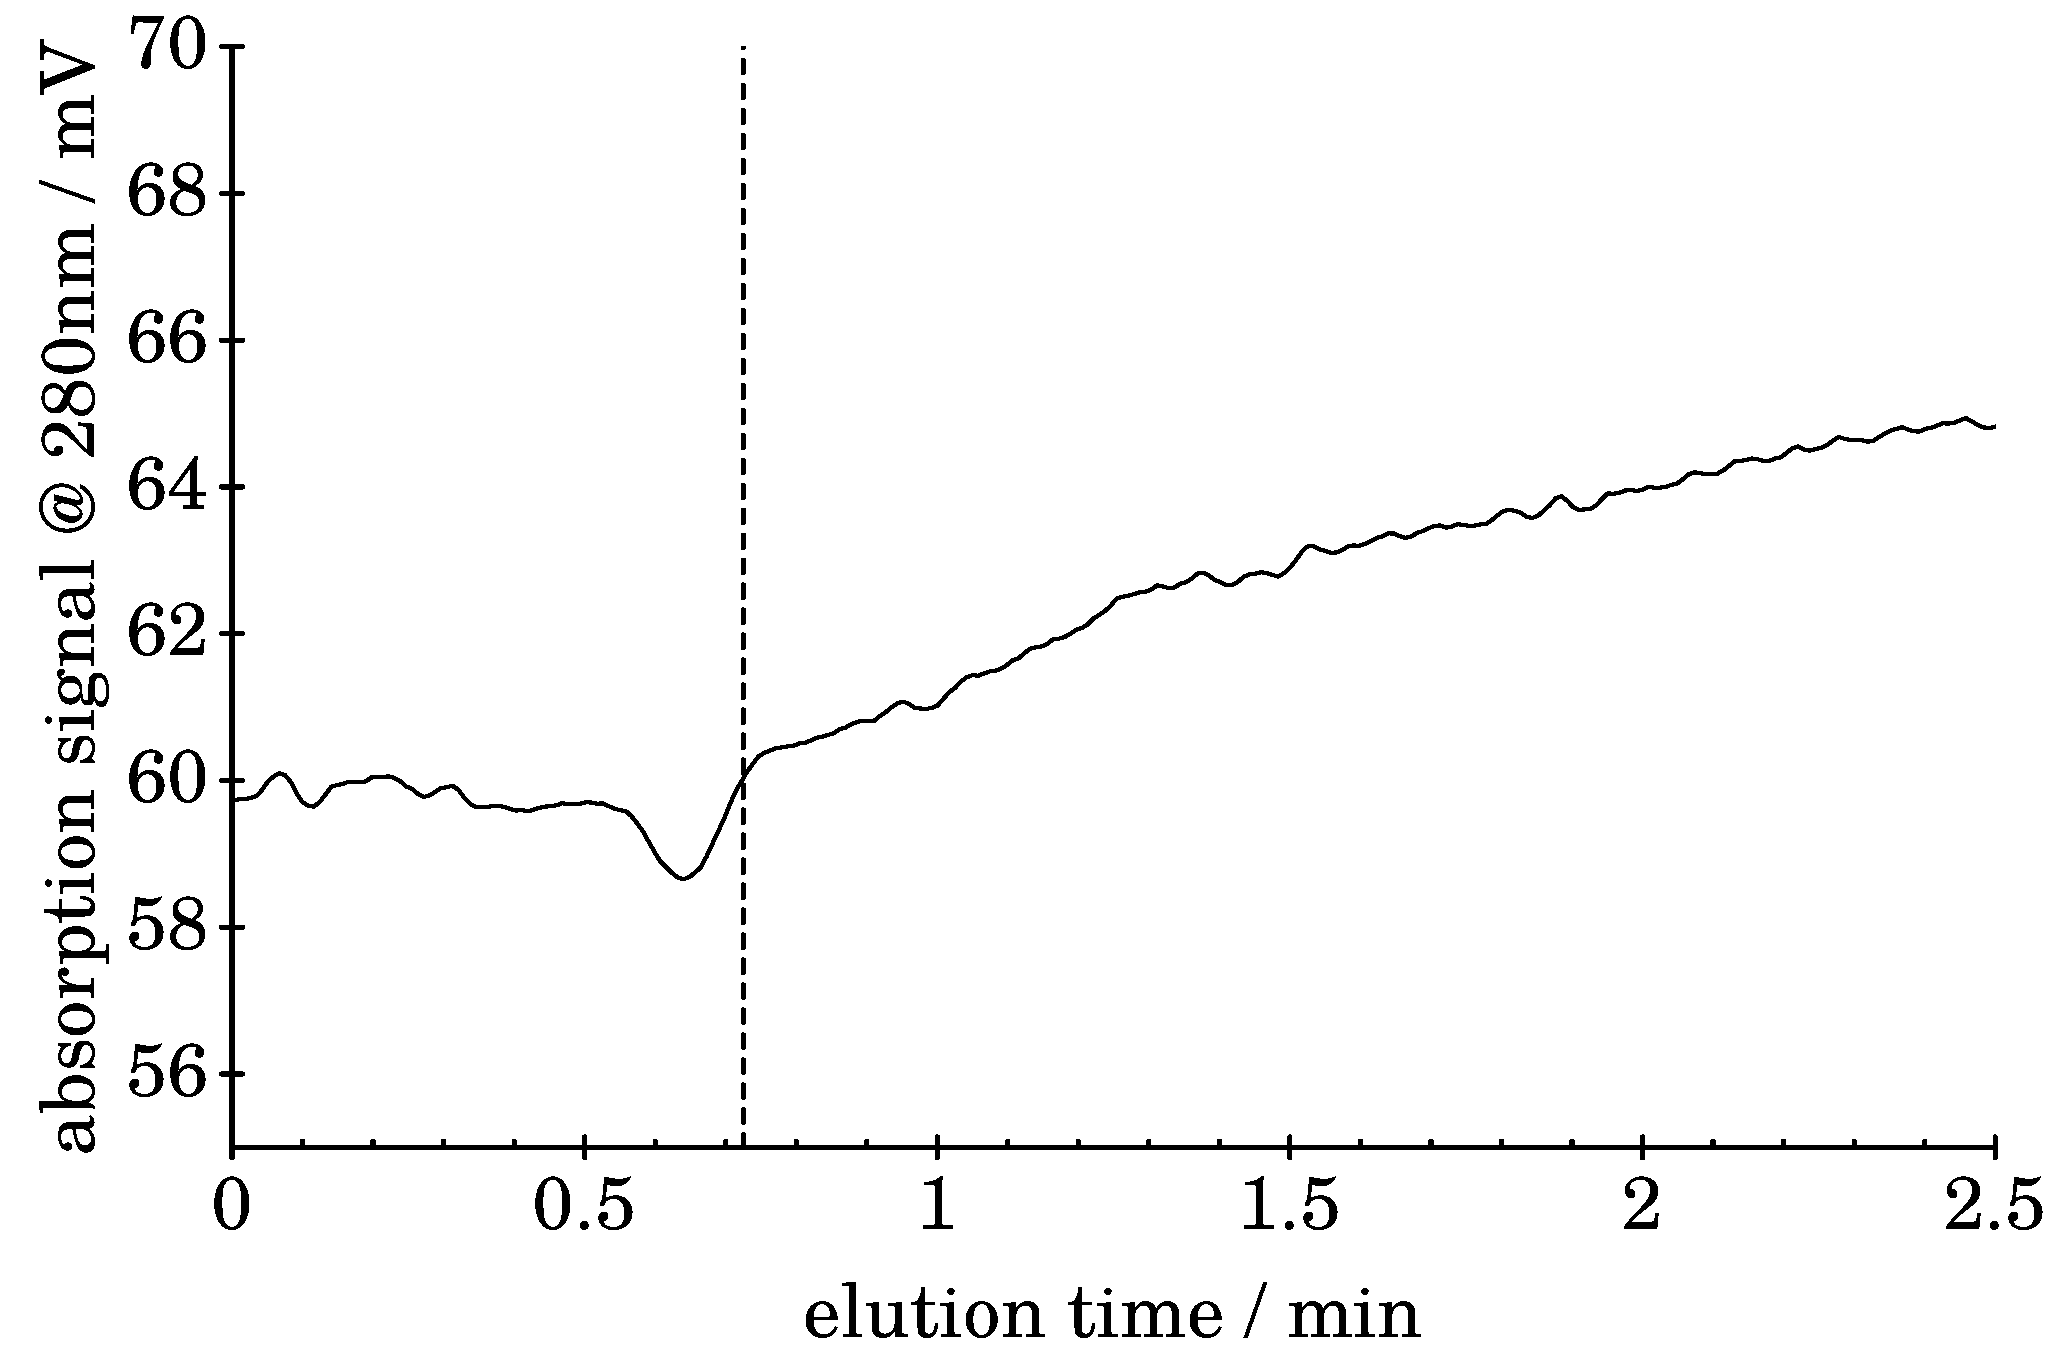
\includegraphics[width=\linewidth]{./images/data/img_PS_VC_05_rep1_t0_UV.pdf}
      \subcaption{Detailed starting section of fractogram \ref{subfig:raw_PS2_5_r1_te_UV}
         with UV detection signal and position of $\tvoid$.}
    \end{subfigure}
  %%%%%%%%%%%%%%%%%%
    \\\vspace*{.5em}
  %%%%%%%%%%%%%%
  \begin{subfigure}{\subFigSize} 
    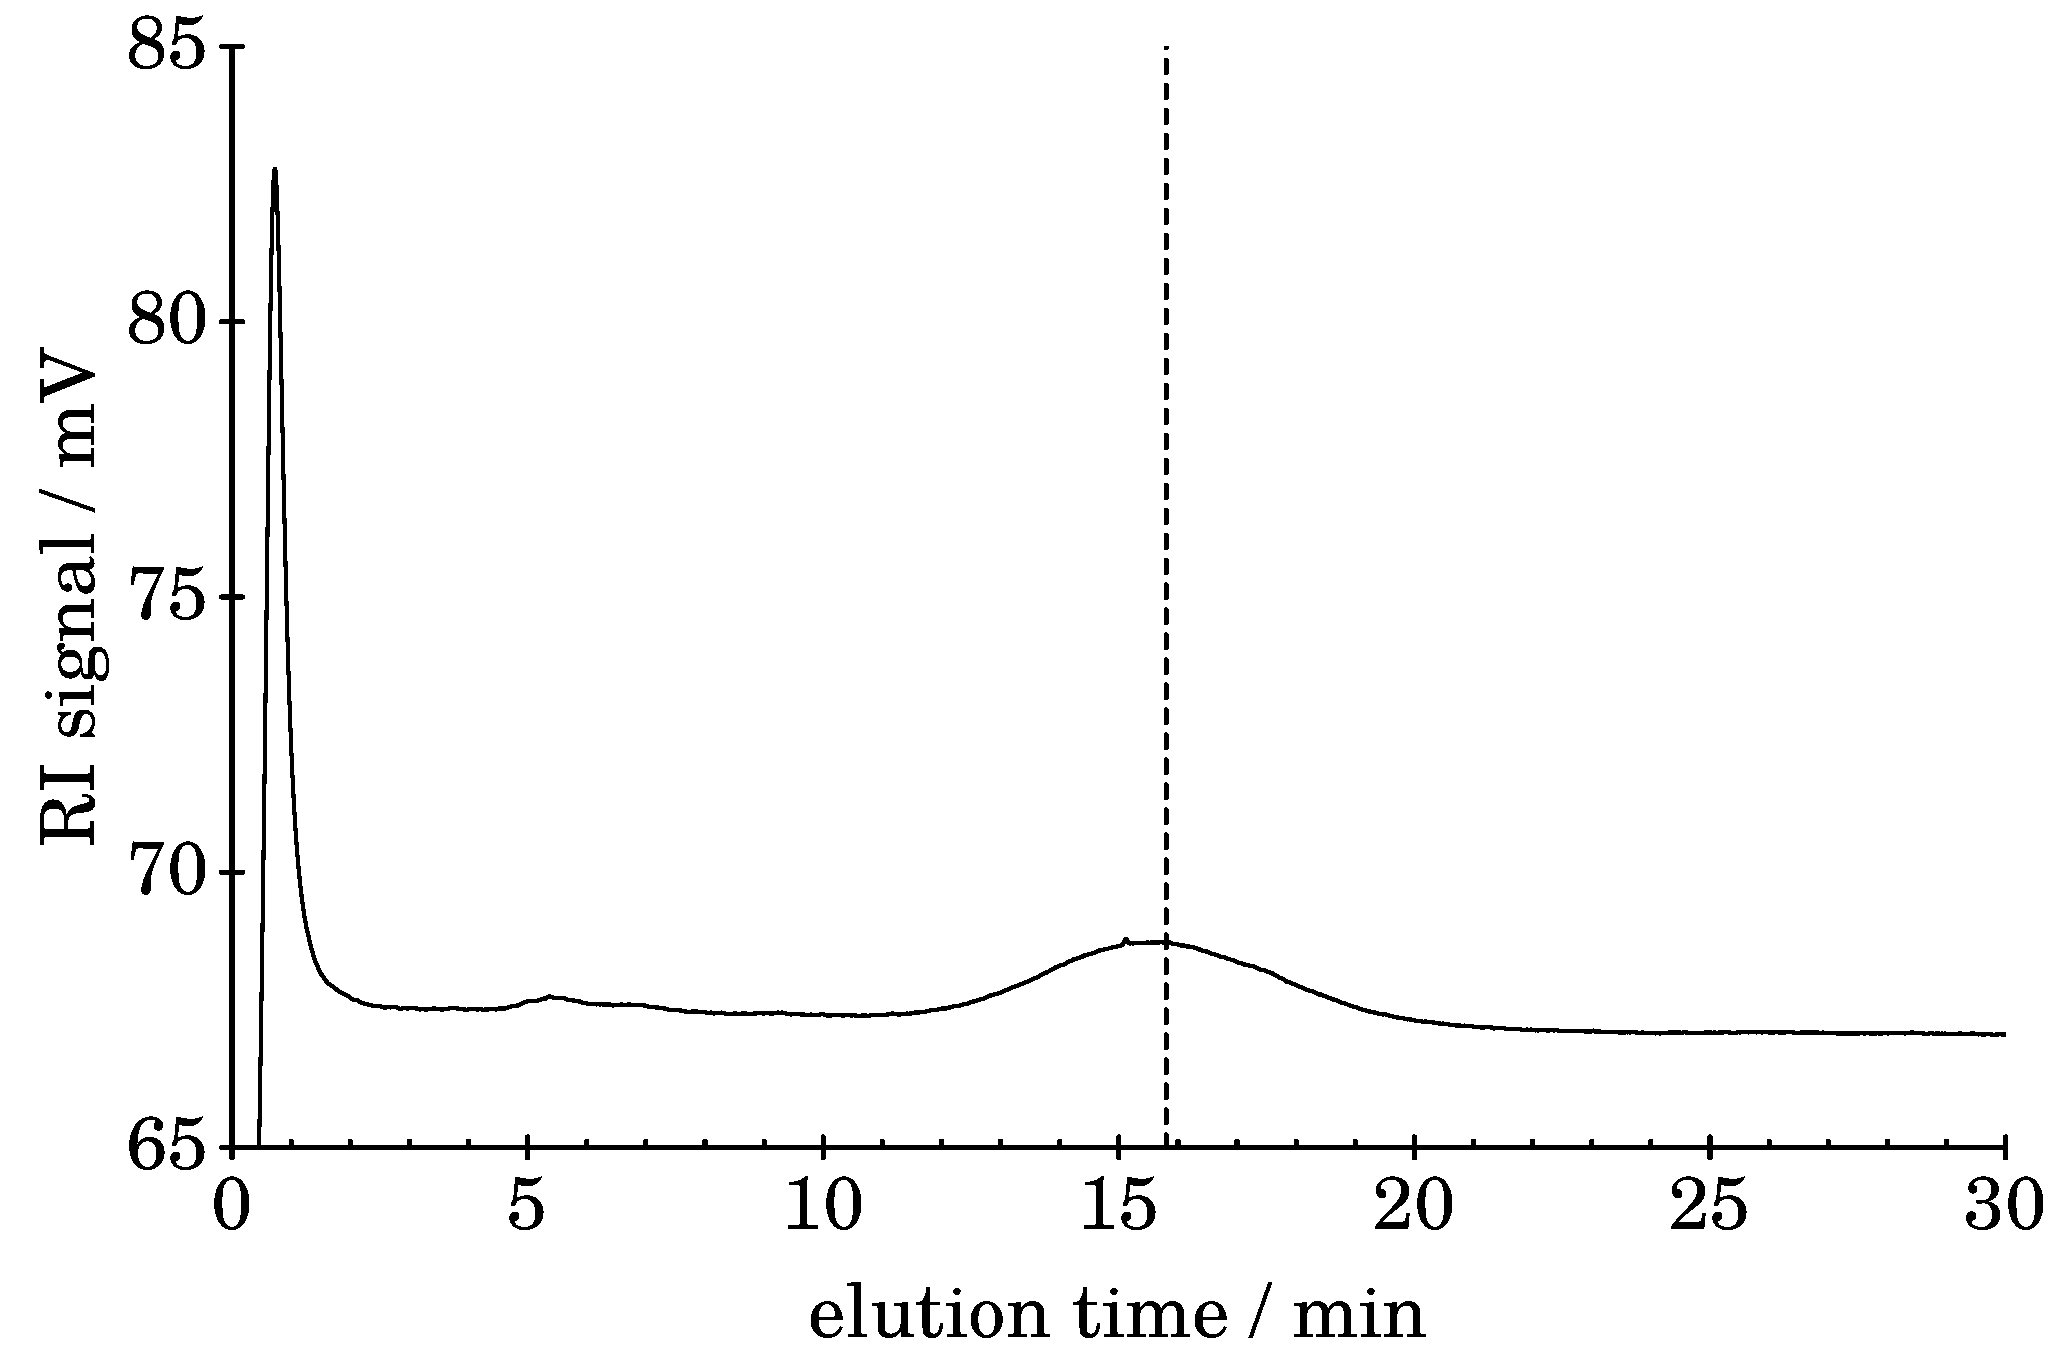
\includegraphics[width=\linewidth]{./images/data/img_PS_VC_05_rep1_te_RI.pdf}
    \subcaption{Position of $\te$ with RI detection signal}
    \label{subfig:raw_PS2_5_r1_te_RI}
  \end{subfigure}
  \begin{subfigure}{\subFigSize}
    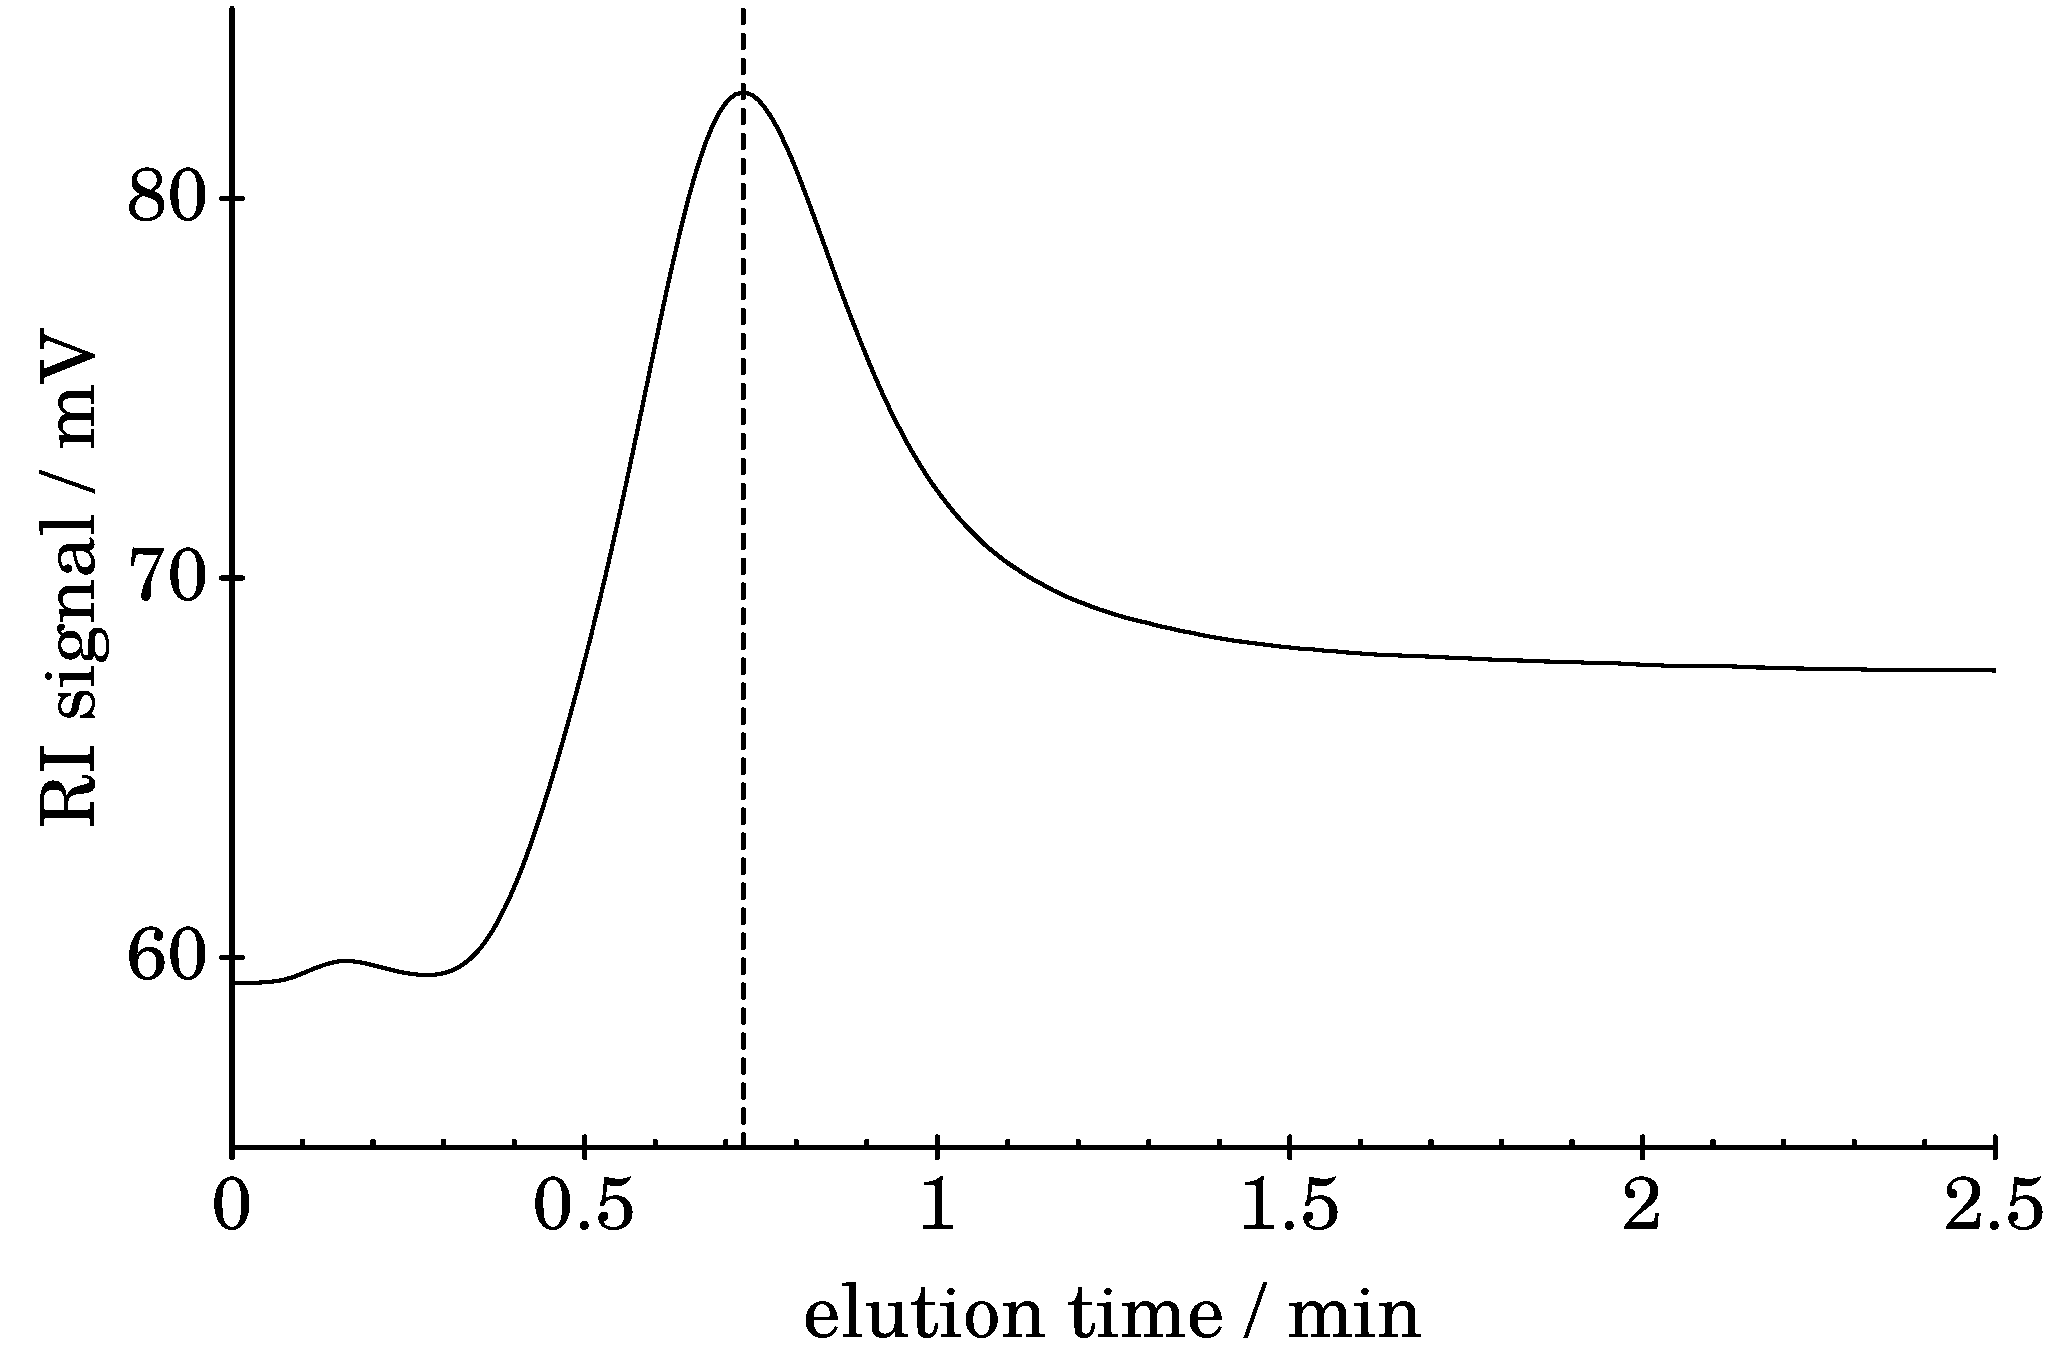
\includegraphics[width=\linewidth]{./images/data/img_PS_VC_05_rep1_t0_RI.pdf}
    \subcaption{Detailed starting section of fractogram \ref{subfig:raw_PS2_5_r1_te_RI}
  with RI detection signal and position of $\tvoid$.}
\end{subfigure}
  \end{center}
\vspace*{-3ex}    
\caption[Raw fractograms of PS measurements at $\Vc = \SI{0.5}{\mlmin}$, replicate 1.]{
Raw fractograms of PS 
measurements at $\Vc = \SI{0.5}{\mlmin}$, replicate 1.}
\label{fig:raw_PS_0_5_rep1} 
\end{figure}\needspace{10ex}
%%%%%%%%%%%%%%%%%%%%%%%%%%%%%%%%%%%%%%%%%%5
%%% PS at Vc = 0.5 ml/min, replicate 2
%%%%%%%%%%%%%%%%%%%%%%%%%%%%%%%%%%%%%%%%
\begin{figure}[b!]
  \begin{center}
    \begin{subfigure}{\subFigSize}
      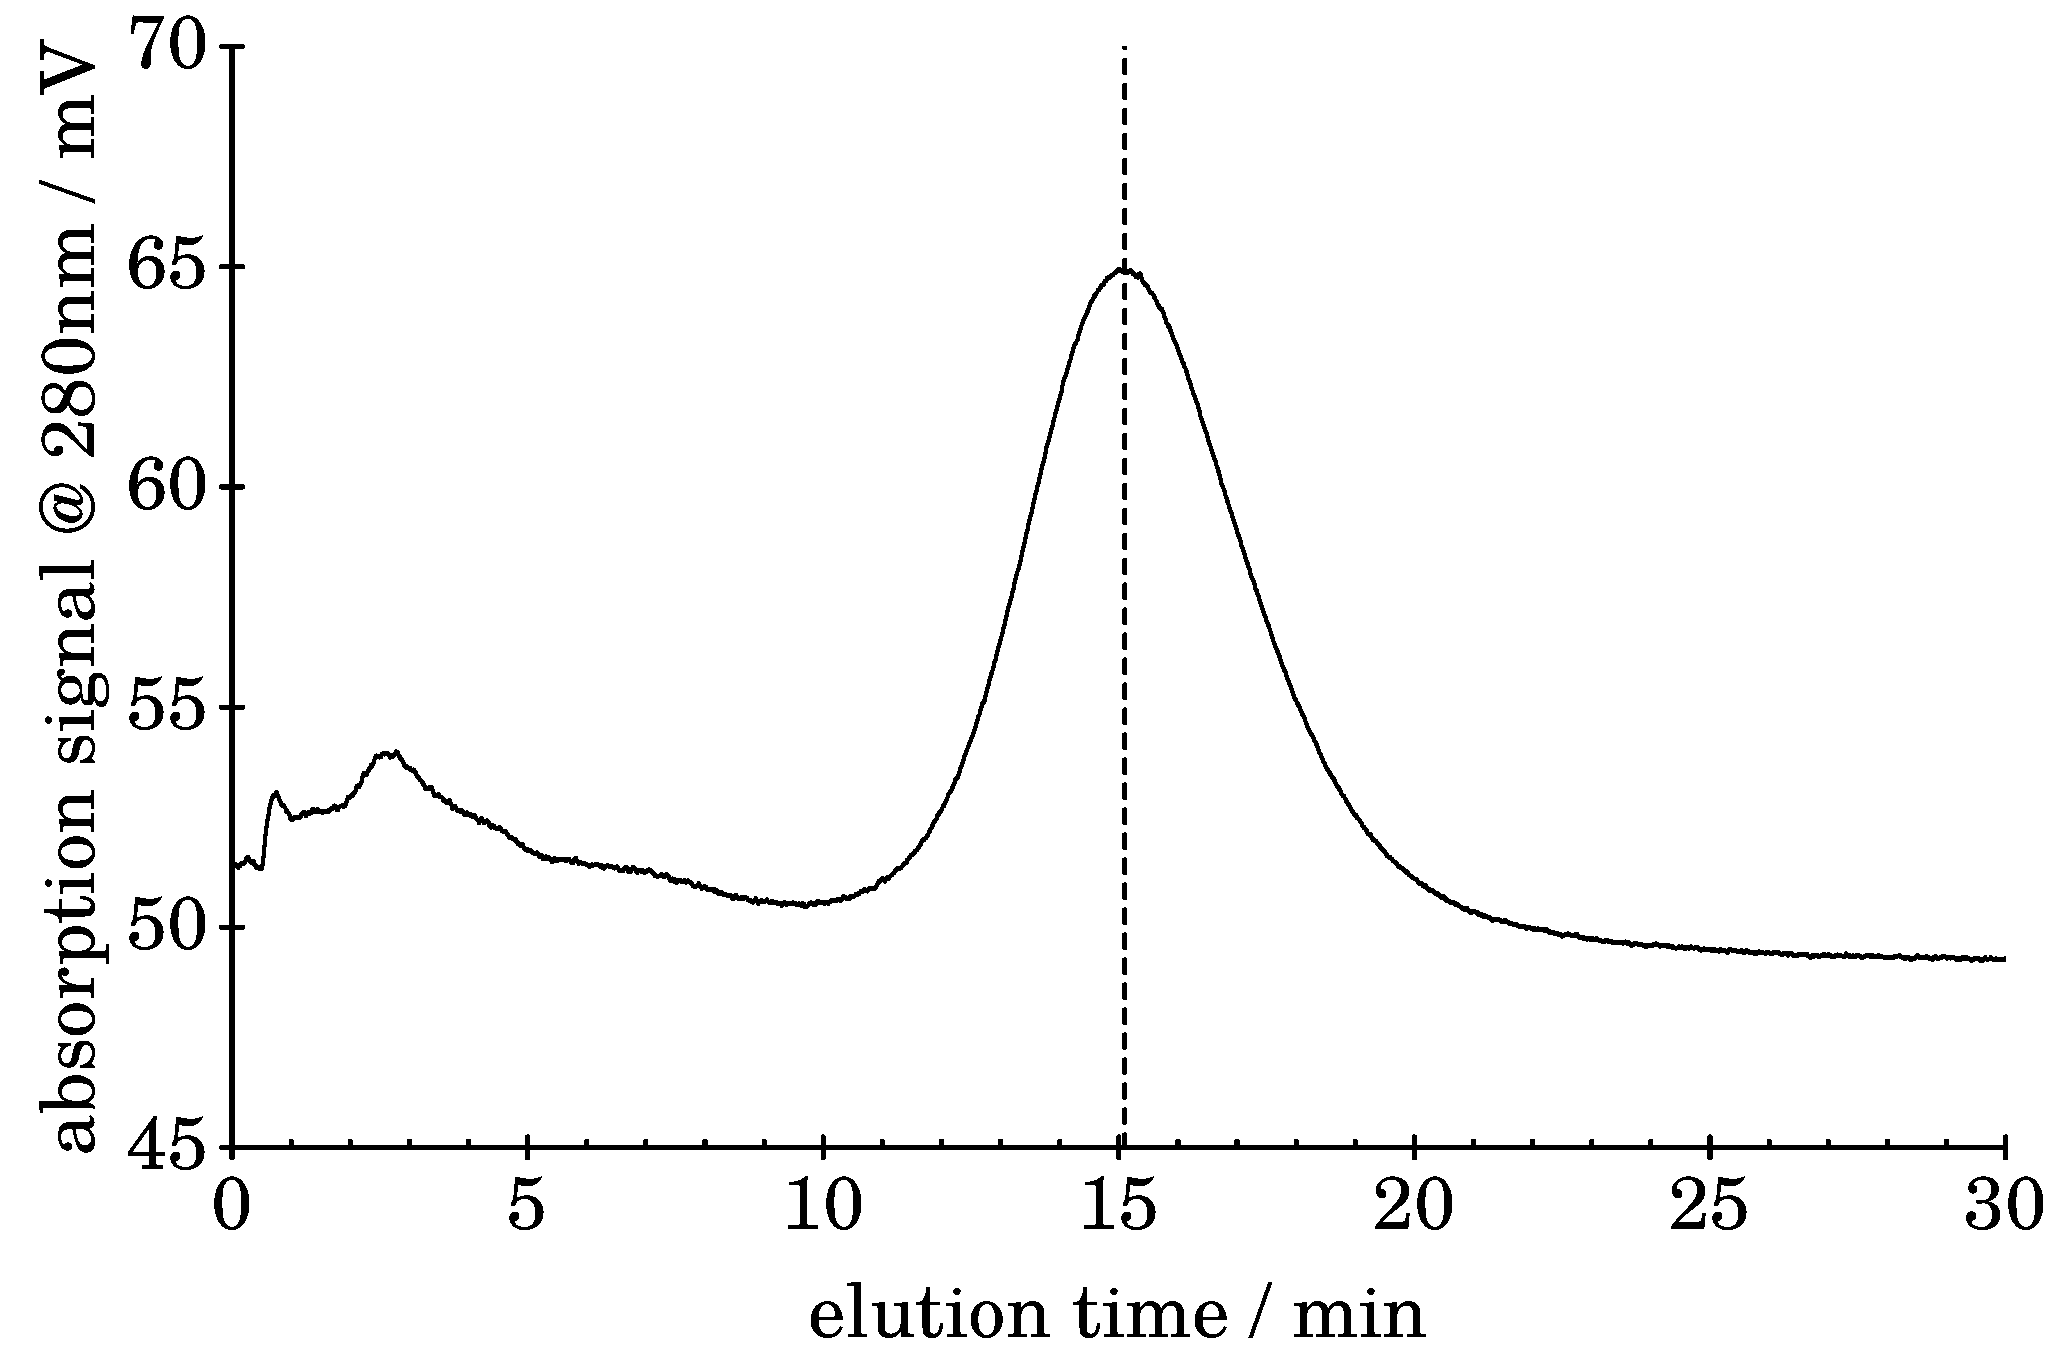
\includegraphics[width=\linewidth]{./images/data/img_PS_VC_05_rep2_te_UV.pdf}
      \subcaption{Position of $\te$ with UV detection signal}
      \label{subfig:raw_PS2_5_r2_te_UV}
    \end{subfigure}
    \begin{subfigure}{\subFigSize}
      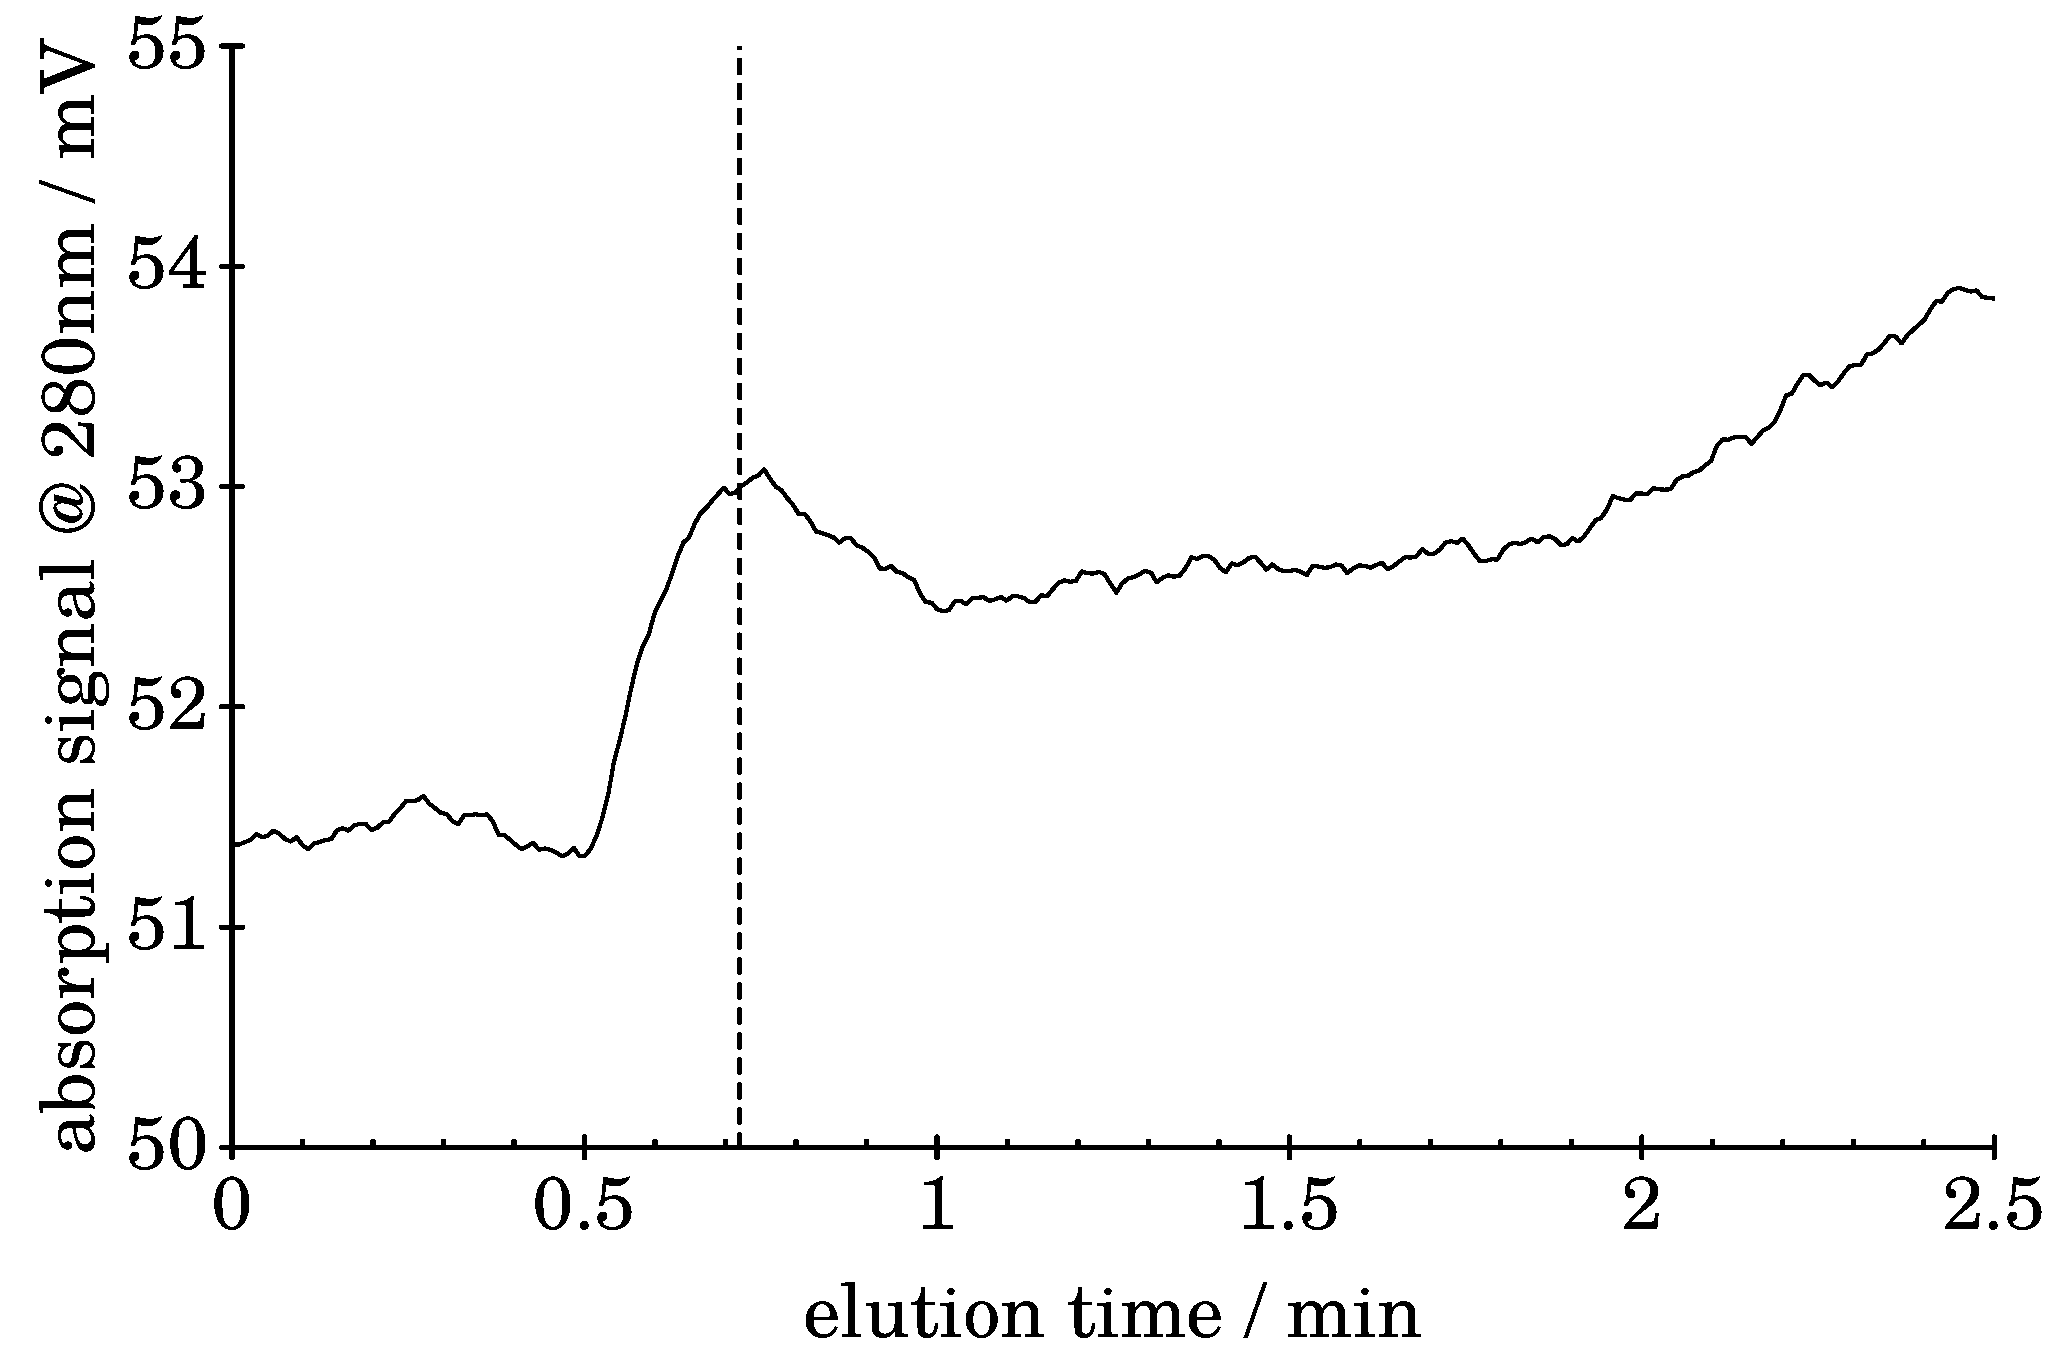
\includegraphics[width=\linewidth]{./images/data/img_PS_VC_05_rep2_t0_UV.pdf}
      \subcaption{Detailed starting section of fractogram \ref{subfig:raw_PS2_5_r2_te_UV}
        with UV detection signal and position of $\tvoid$.}
    \end{subfigure}
    %%%%%%%%%%%%%%%%%%
    \\\vspace*{.5em}
    %%%%%%%%%%%%%%
    \begin{subfigure}{\subFigSize} 
      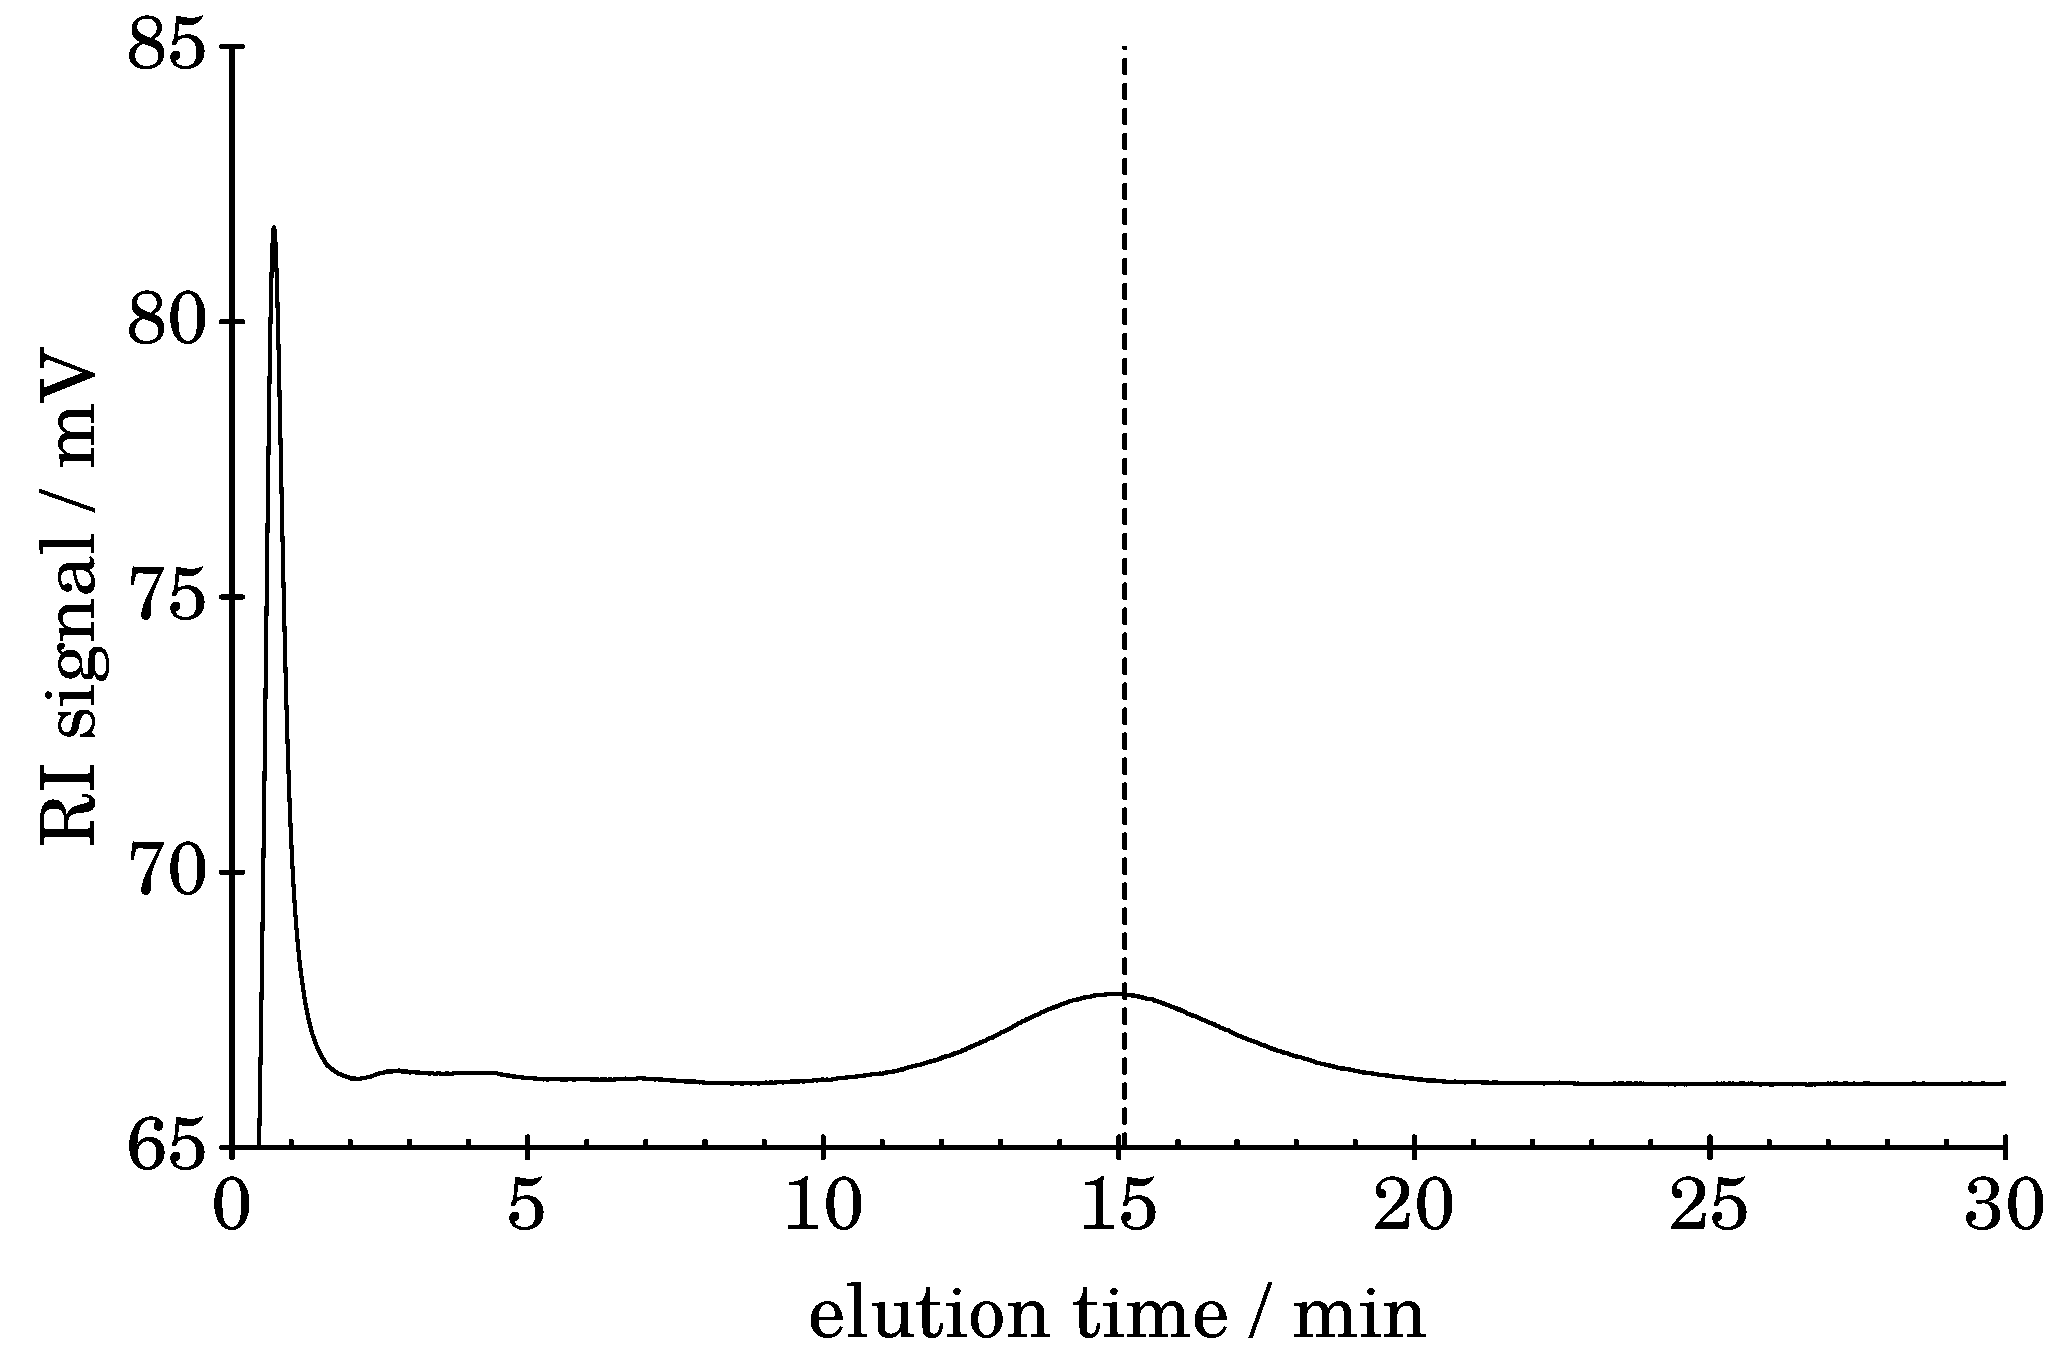
\includegraphics[width=\linewidth]{./images/data/img_PS_VC_05_rep2_te_RI.pdf}
      \subcaption{Position of $\te$ with RI detection signal}
      \label{subfig:raw_PS2_5_r2_te_RI}
    \end{subfigure}
    \begin{subfigure}{\subFigSize}
      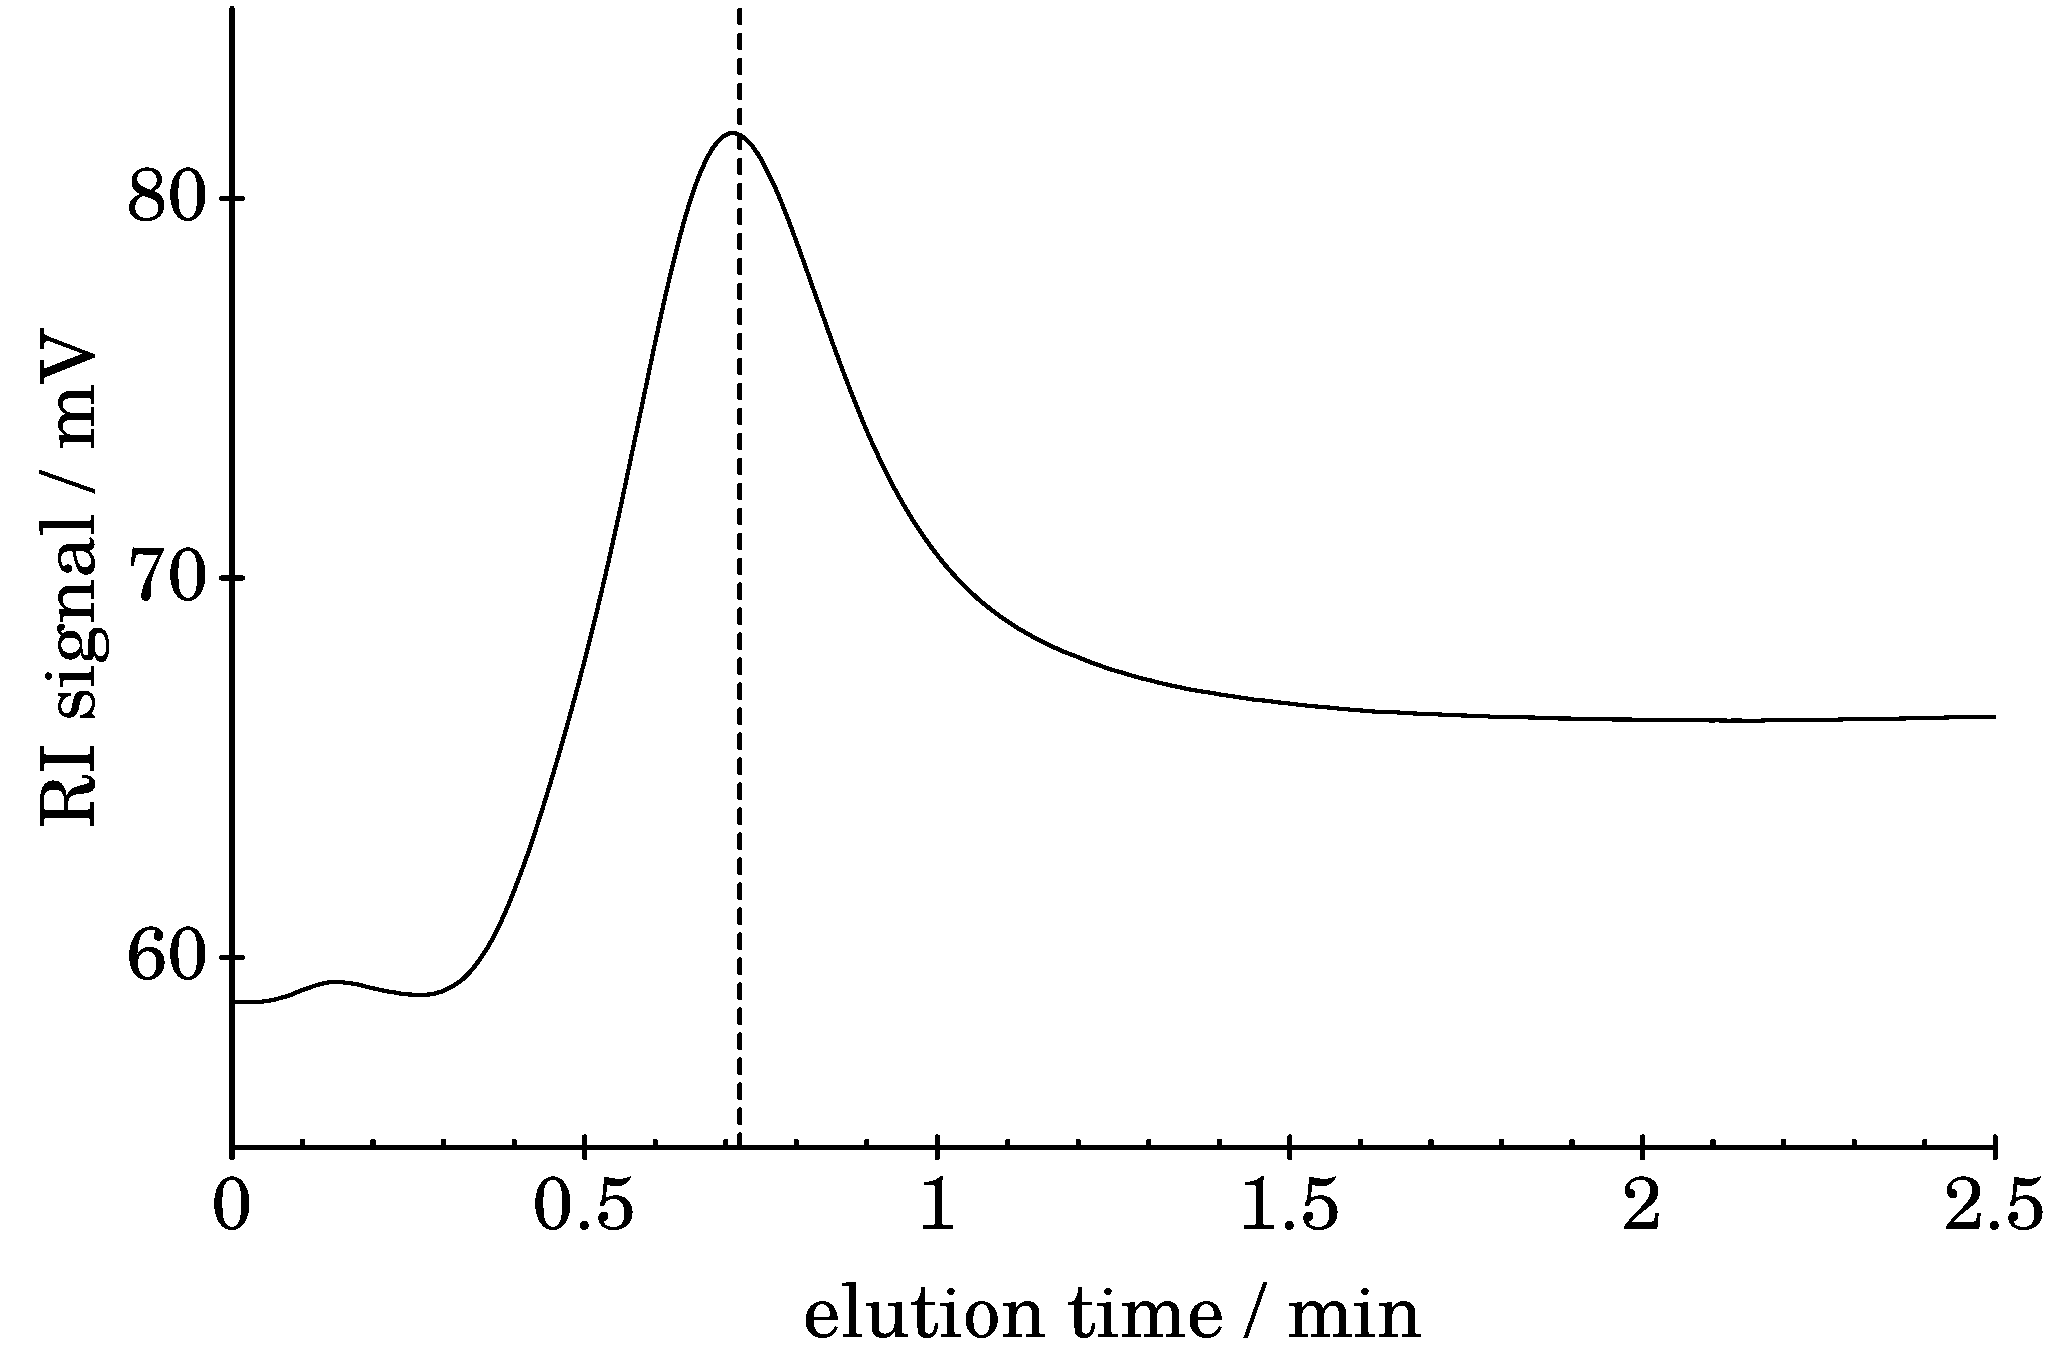
\includegraphics[width=\linewidth]{./images/data/img_PS_VC_05_rep2_t0_RI.pdf}
      \subcaption{Detailed starting section of fractogram \ref{subfig:raw_PS2_5_r2_te_RI}
        with RI detection signal and position of $\tvoid$.}
    \end{subfigure}
  \end{center}
  \vspace*{-3ex}    
  \caption[Raw fractograms of PS measurements at $\Vc = \SI{0.5}{\mlmin}$, replicate 2.]{
    Raw fractograms of PS 
    measurements at $\Vc = \SI{0.5}{\mlmin}$, replicate 2.}
  \label{fig:raw_PS_0_5_rep2} 
\end{figure}
%%%%%%%%%%%%%%%%%%%%%%%%%%%%%%%%%%%%%%%%%
%%% PS at Vc = 0.5 ml/min, replicate 3
%%%%%%%%%%%%%%%%%%%%%%%%%%%%%%%%%%%%%%%%
\begin{figure}[H]
  \begin{center}
    \begin{subfigure}{\subFigSize}
      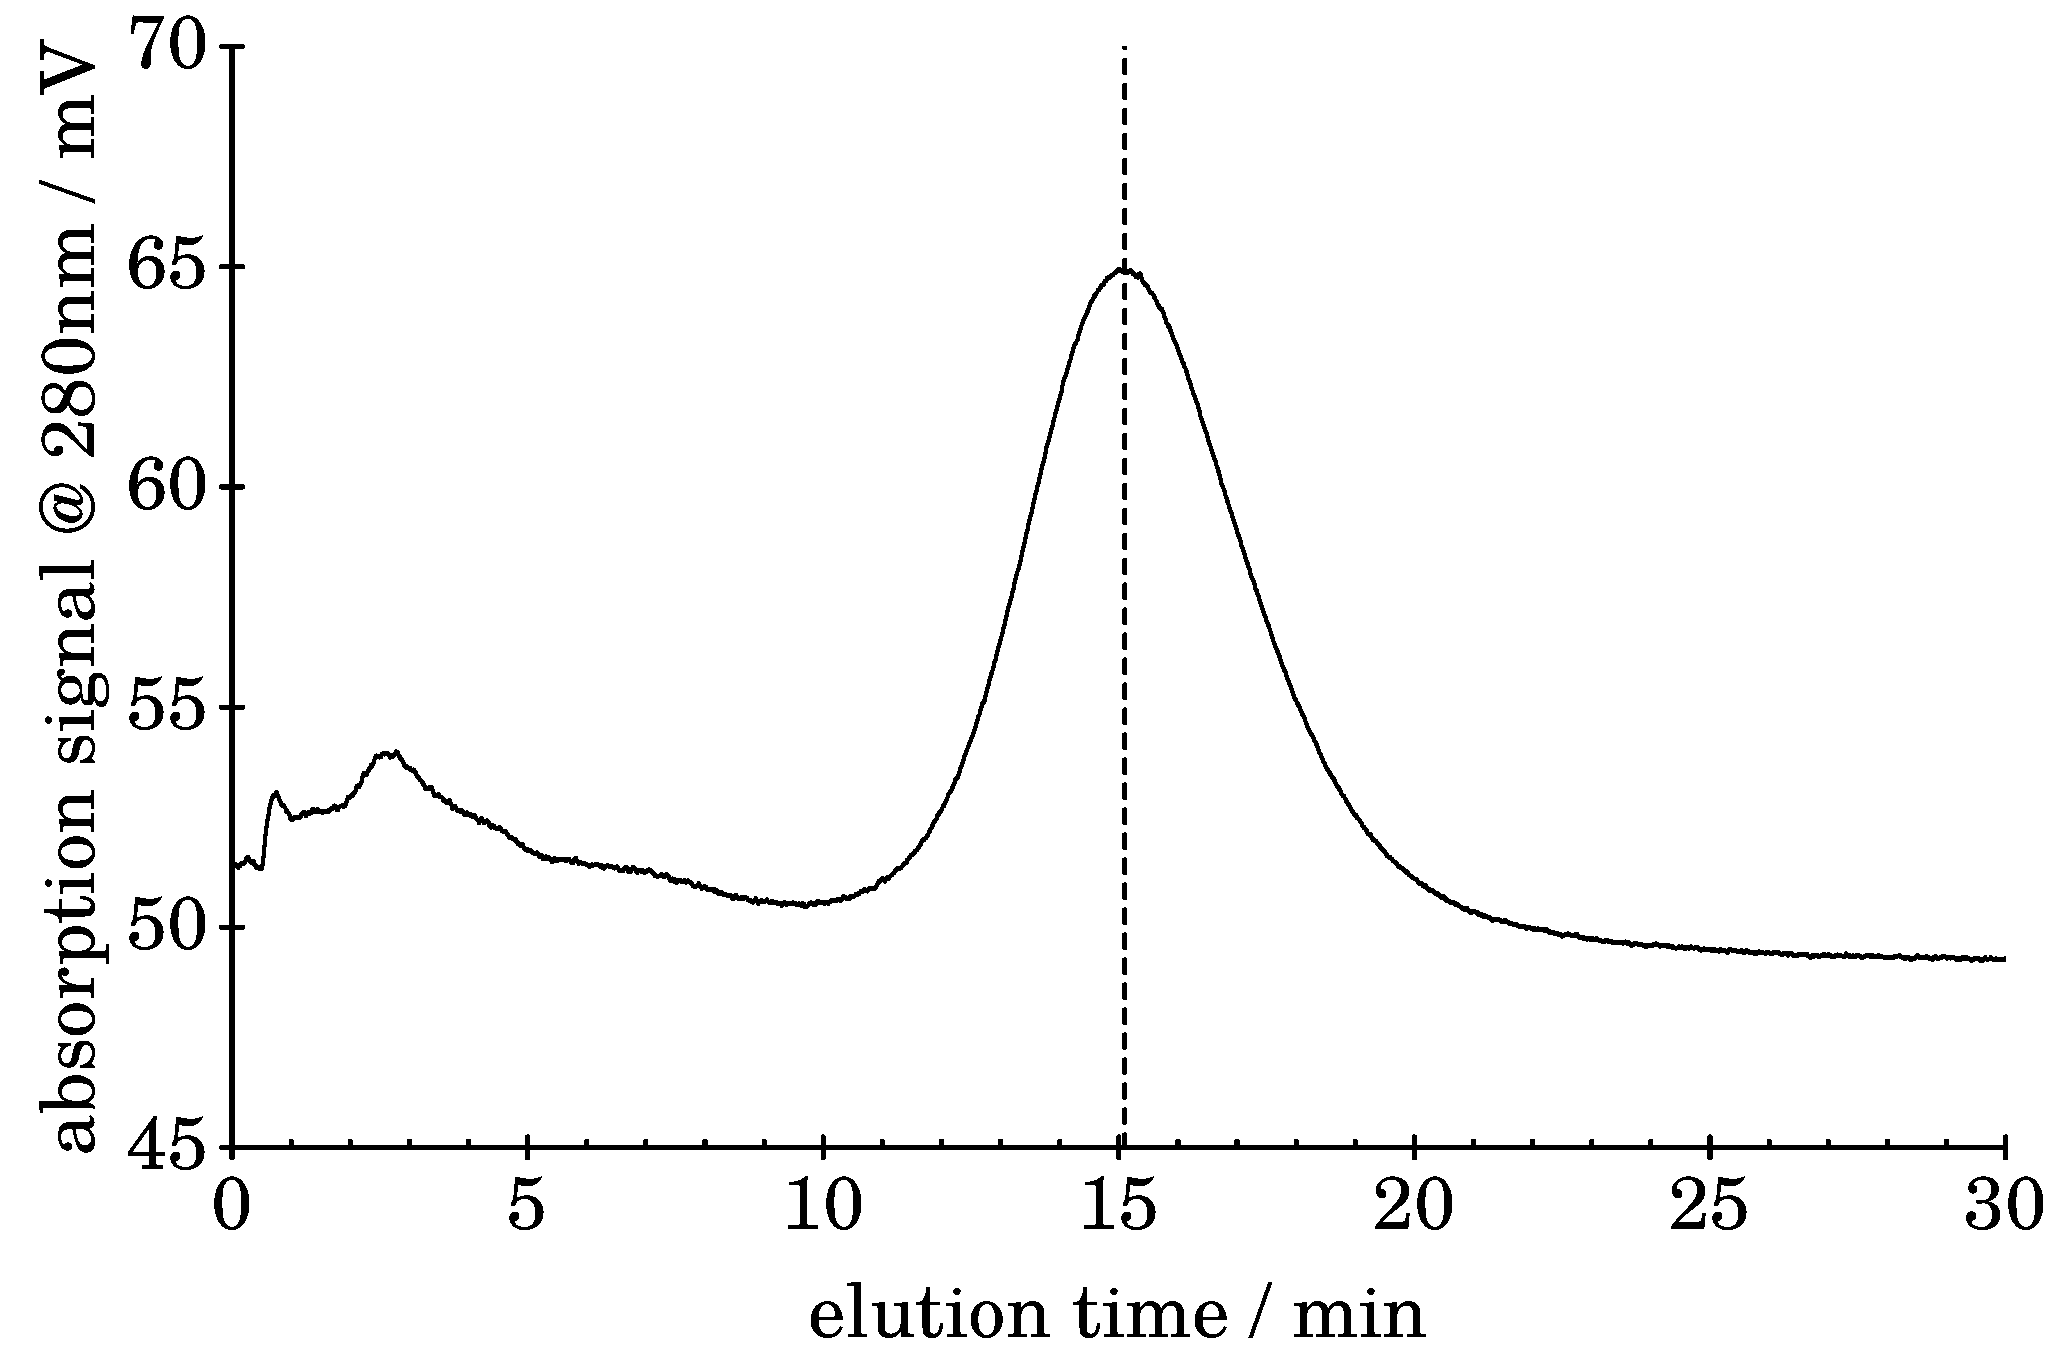
\includegraphics[width=\linewidth]{./images/data/img_PS_VC_05_rep2_te_UV.pdf}
      \subcaption{Position of $\te$ with UV detection signal}
      \label{subfig:raw_PS2_5_r3_te_UV}
    \end{subfigure}
    \begin{subfigure}{\subFigSize}
      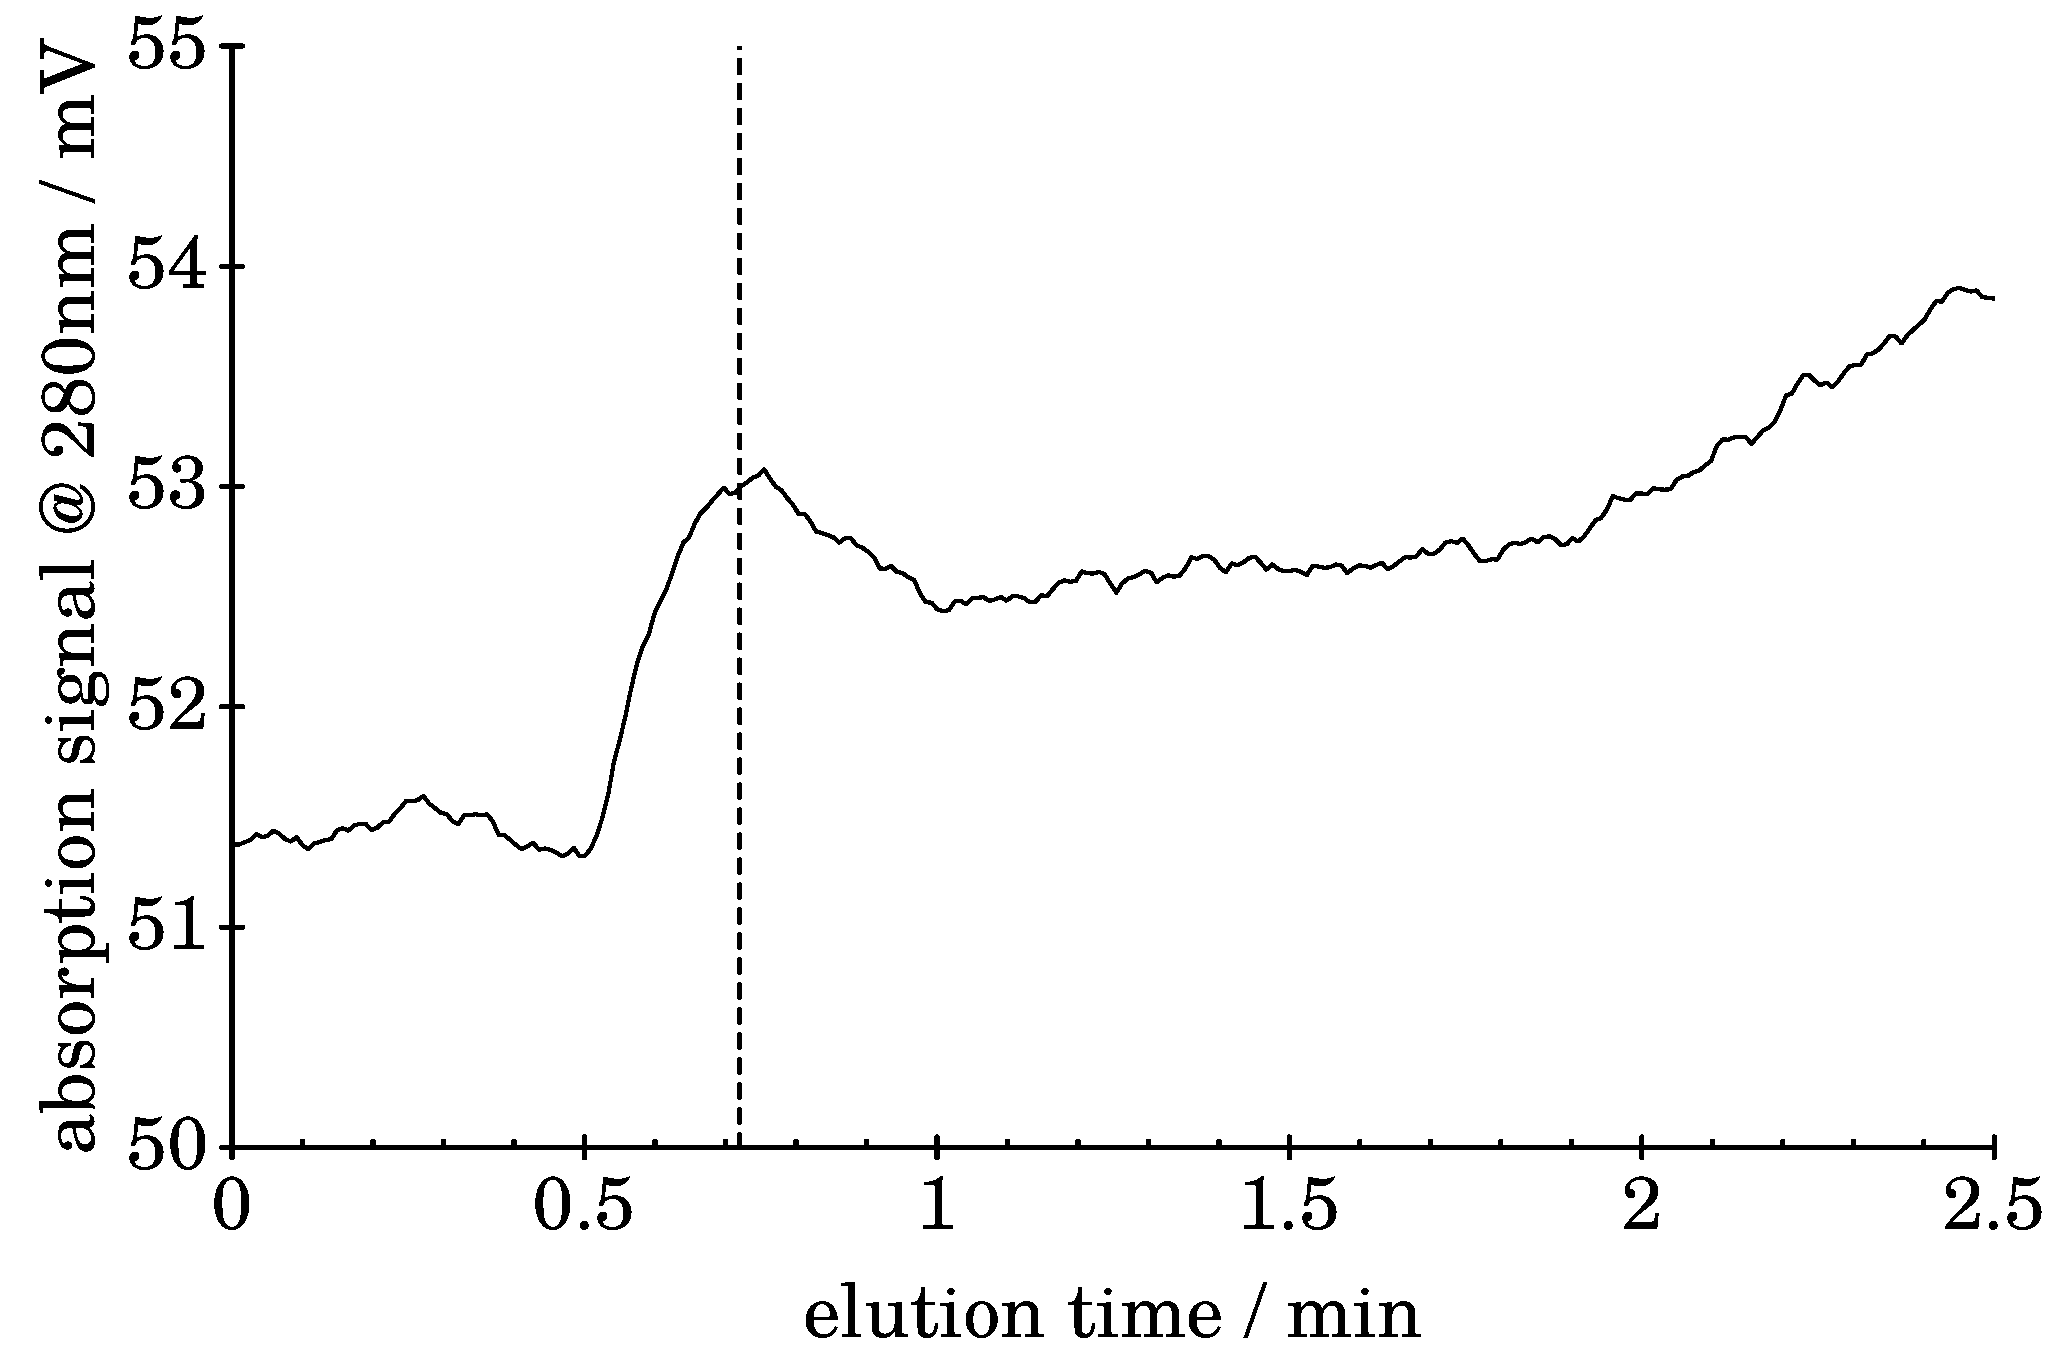
\includegraphics[width=\linewidth]{./images/data/img_PS_VC_05_rep2_t0_UV.pdf}
      \subcaption{Detailed starting section of fractogram \ref{subfig:raw_PS2_5_r3_te_UV}
        with UV detection signal and position of $\tvoid$.}
    \end{subfigure}
    %%%%%%%%%%%%%%%%%%
    \\\vspace*{.5em}
    %%%%%%%%%%%%%%
    \begin{subfigure}{\subFigSize} 
      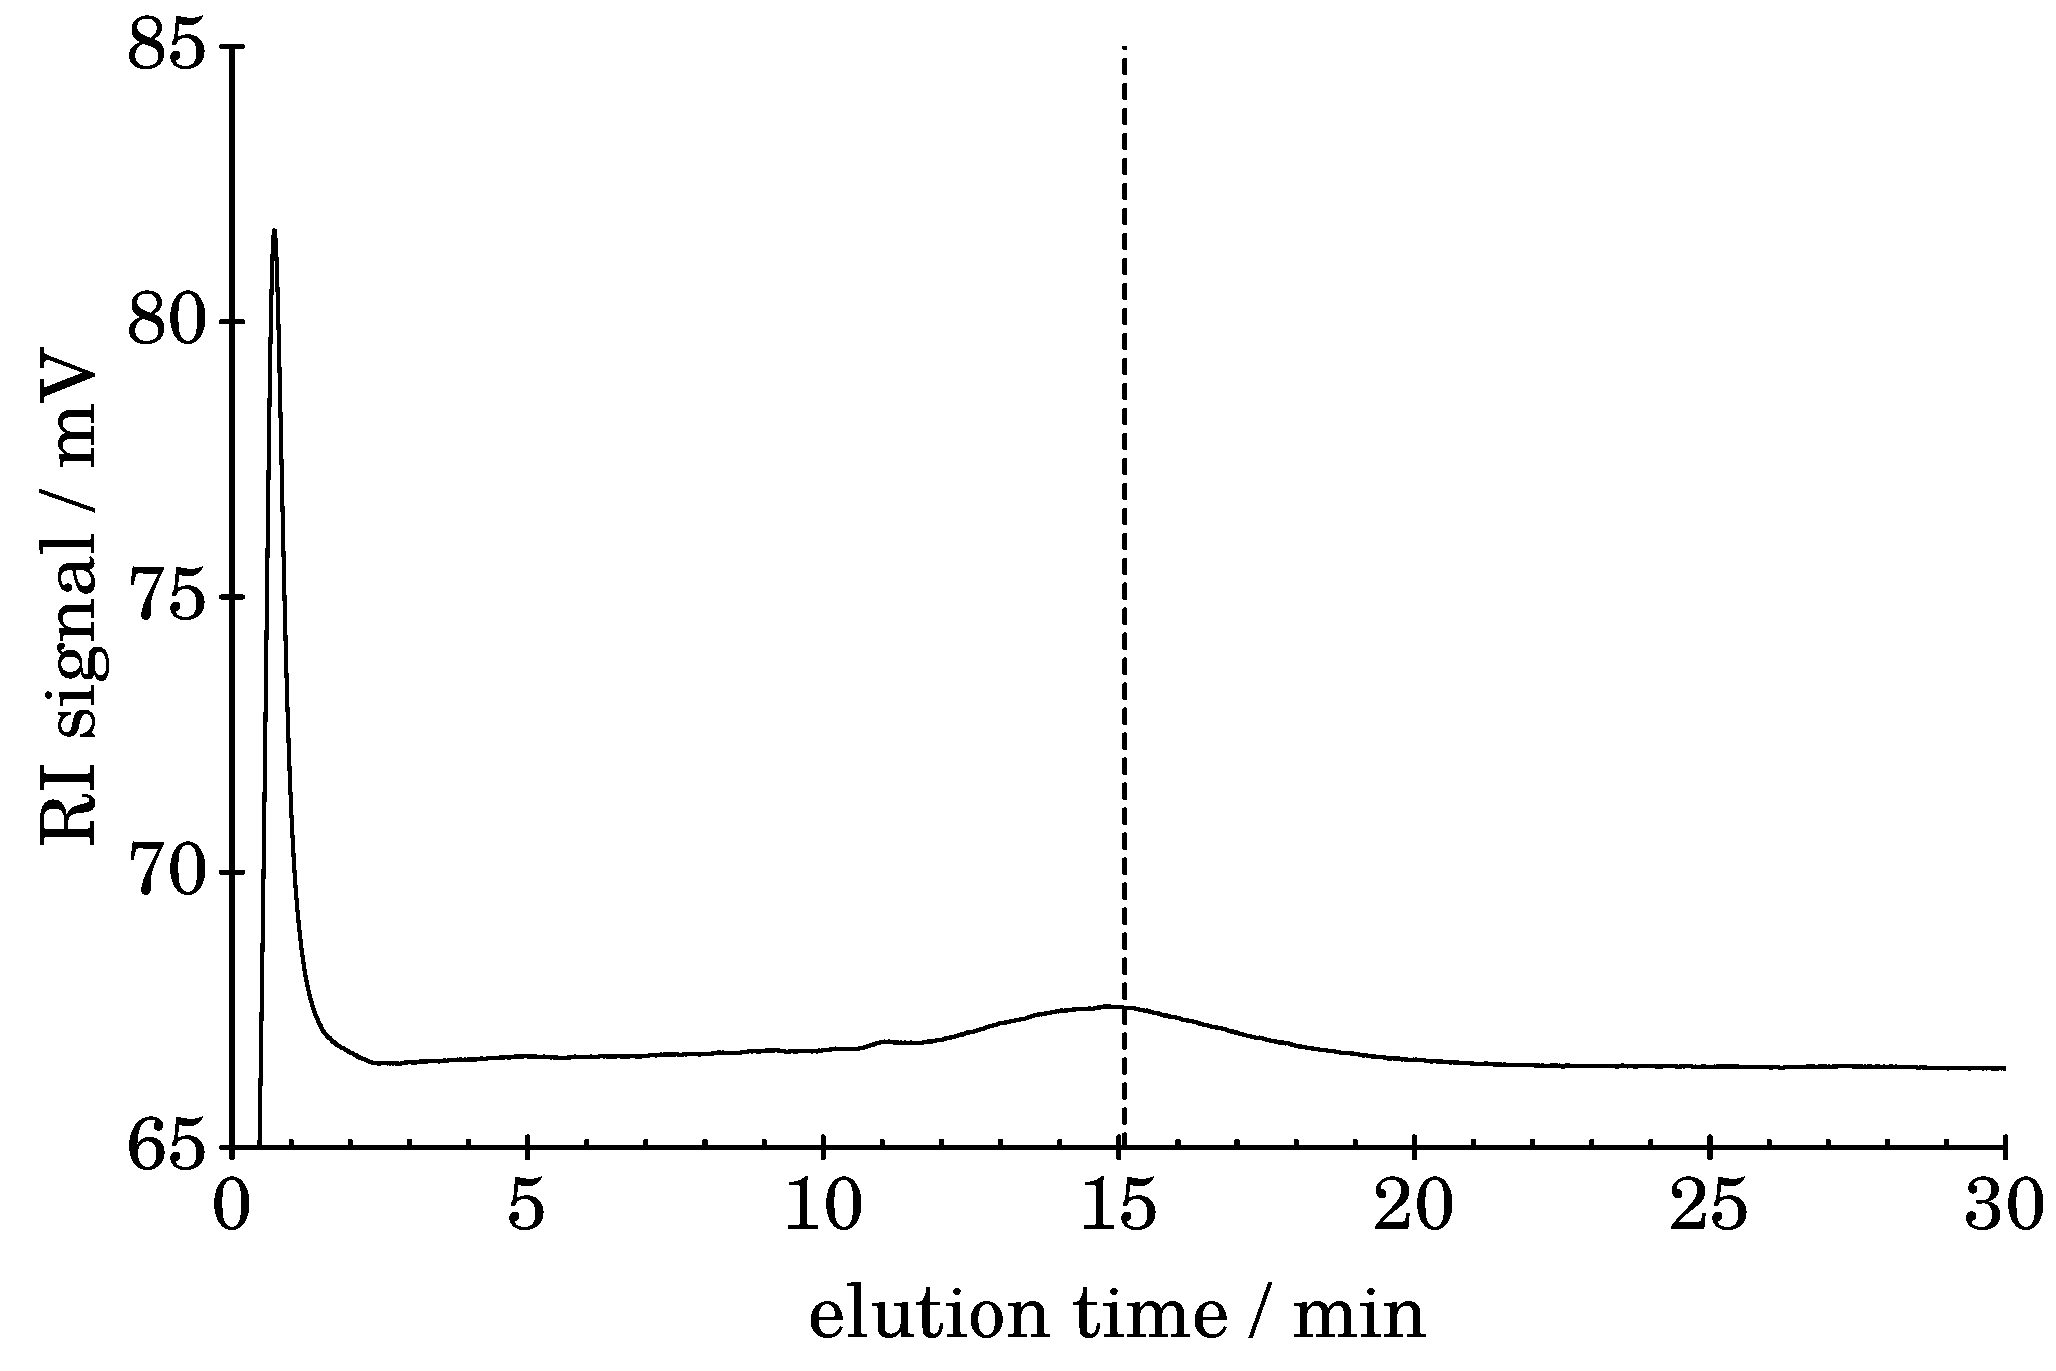
\includegraphics[width=\linewidth]{./images/data/img_PS_VC_05_rep3_te_RI.pdf}
      \subcaption{Position of $\te$ with RI detection signal}
      \label{subfig:raw_PS2_5_r3_te_RI}
    \end{subfigure}
    \begin{subfigure}{\subFigSize}
      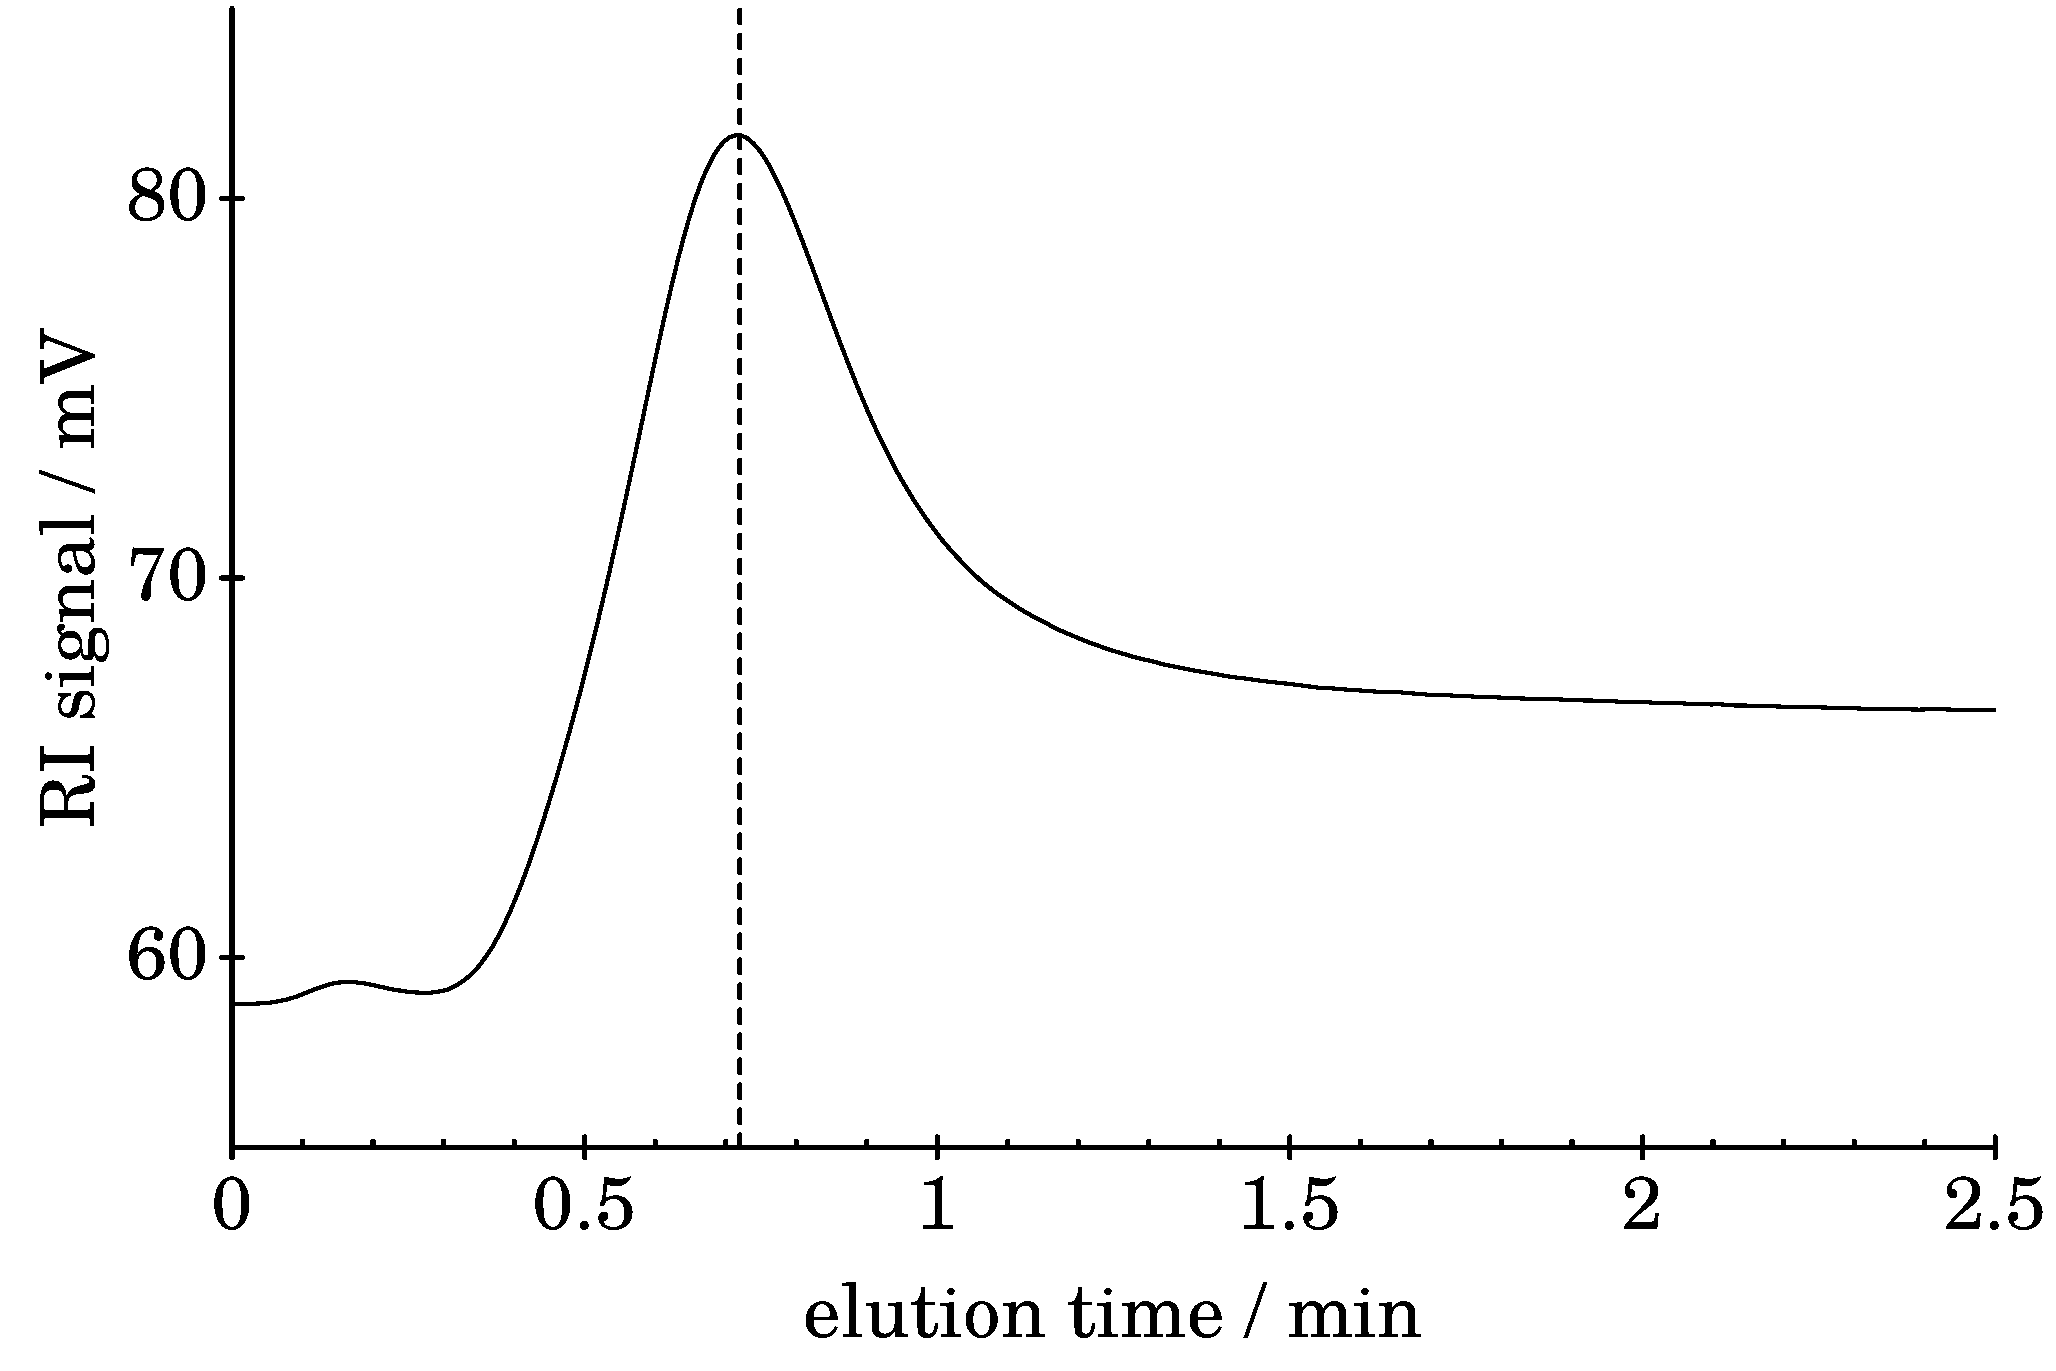
\includegraphics[width=\linewidth]{./images/data/img_PS_VC_05_rep3_t0_RI.pdf}
      \subcaption{Detailed starting section of fractogram \ref{subfig:raw_PS2_5_r3_te_RI}
        with RI detection signal and position of $\tvoid$.}
    \end{subfigure}
  \end{center}
  \vspace*{-3ex}    
  \caption[Raw fractograms of PS measurements at $\Vc = \SI{0.5}{\mlmin}$, replicate 3.]{
    Raw fractograms of PS 
    measurements at $\Vc = \SI{0.5}{\mlmin}$, replicate 3.}
  \label{fig:raw_PS_0_5_rep3}
\end{figure}
%\newgeometry{bottom=0.5cm}
%\newgeometry{foot=0.5cm}
\clearpage
\section*{Evaluated results of calibration experiments with BSA and PS}
\renewcommand{\subFigSize}{0.49\linewidth}
%\begin{landscape}
%\thispagestyle{empty}
%%%%%%%%%%%%%%%%%%%%%%%%%%%%%%
%%% BSA, Vc = 2.5 ml/min
%%%%%%%%%%%%%%%%%%%%%%%%%%%%%
%\begin{minipage}[t]{1.1\linewidth}
\begin{figure}[htp]
  \begin{center}
    \begin{subfigure}{\subFigSize}
      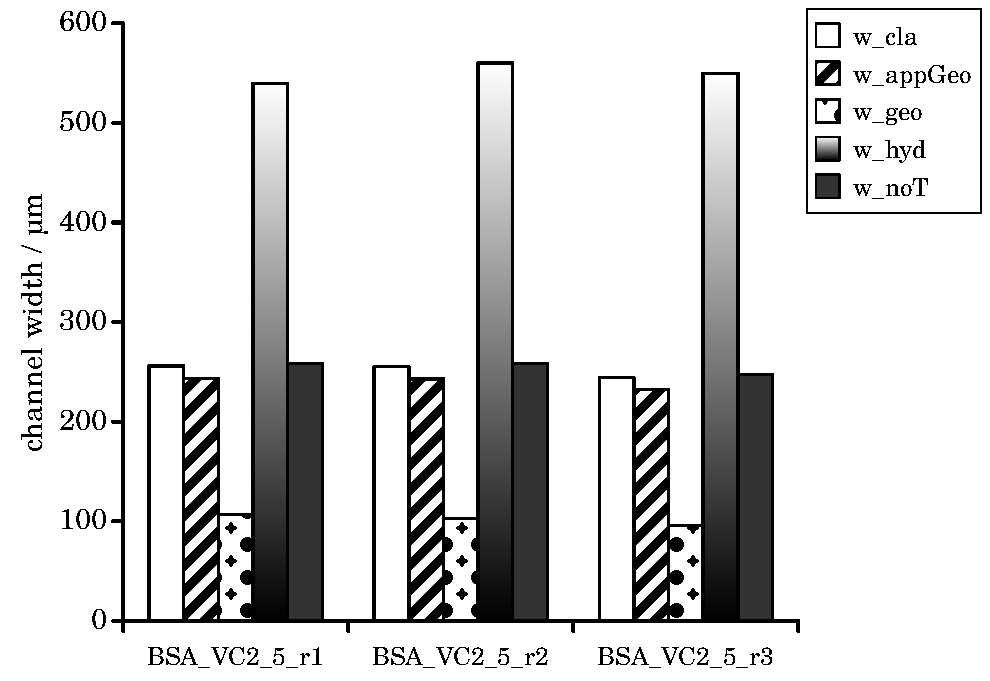
\includegraphics[width=\linewidth]{./images/data/img_calibW_BSA_VC_2_5.pdf}
      \subcaption{Calibration results for $w$}
      \label{subfig:calibRes_BSA_VC2_5_w}
    \end{subfigure}
    \begin{subfigure}{\subFigSize}
      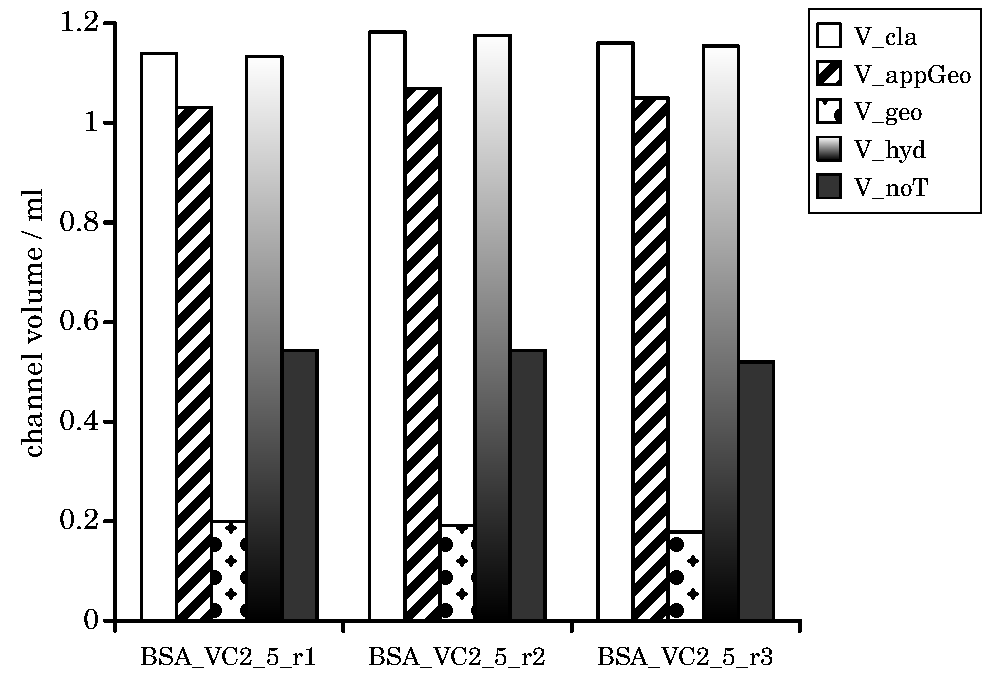
\includegraphics[width=\linewidth]{./images/data/img_calibV_BSA_VC_2_5.pdf}
      \subcaption{Calibration results for $V$}
    \end{subfigure}
  \end{center}
  \vspace*{-4ex}    
  \caption[Results of $w$ and $V$ from all 5 calibration algorithms for BSA measurements at
   $\Vc = \SI{2.5}{\mlmin}$]{
     Results of $w$ and $V$ from all 5 calibration algorithms for BSA measurements at
     $\Vc = \SI{2.5}{\mlmin}$
}
\label{fig:calibRes_BSA_VC2_5}
\end{figure}  
%%%%%%%%%%%%%%%%%%%%%%%%%%%%%%
%%% BSA, Vc = 3.5 ml/min
%%%%%%%%%%%%%%%%%%%%%%%%%%%%%
\begin{figure}[htp]
  \begin{center}
    \begin{subfigure}{\subFigSize}
      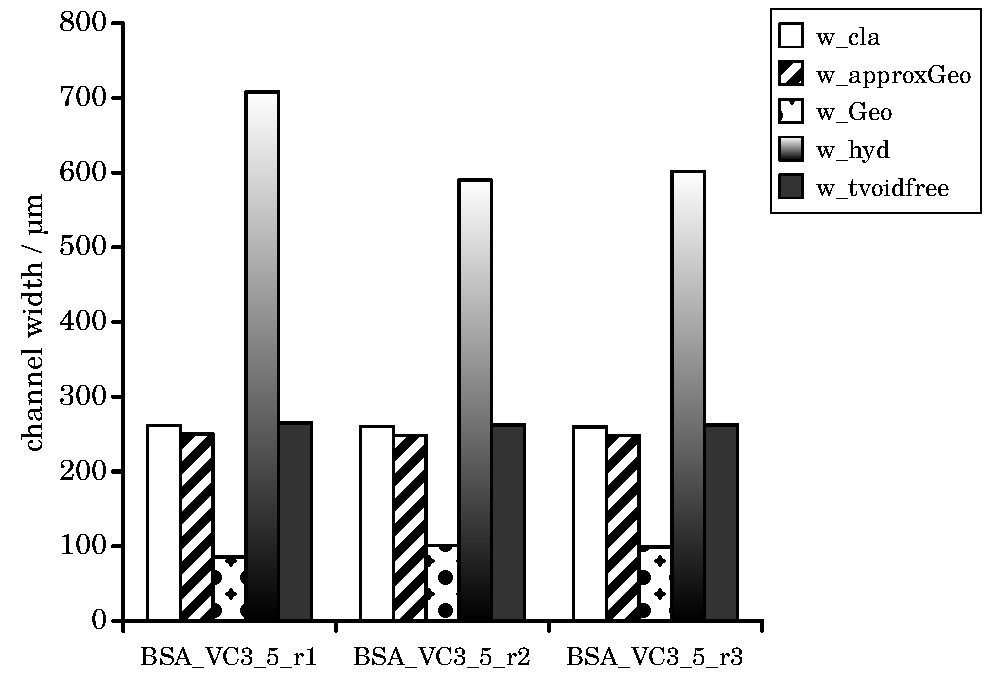
\includegraphics[width=\linewidth]{./images/data/img_calibW_BSA_VC_3_5.pdf}
      \subcaption{Calibration results for $w$}
      \label{subfig:calibRes_BSA_VC3_5_w}
    \end{subfigure}
    \begin{subfigure}{\subFigSize}
      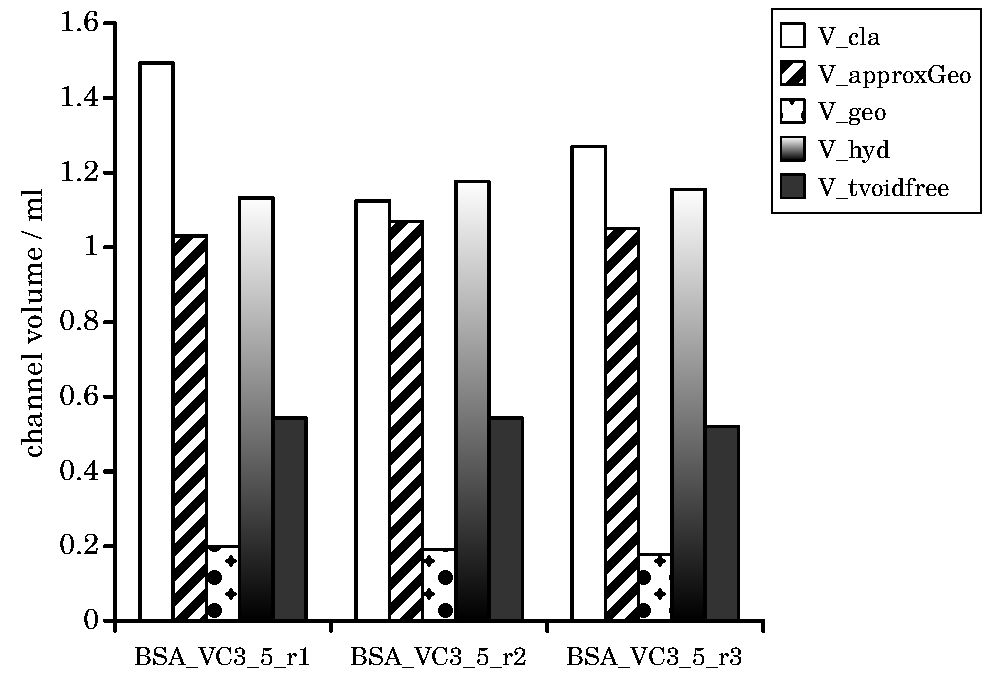
\includegraphics[width=\linewidth]{./images/data/img_calibV_BSA_VC_3_5.pdf}
      \subcaption{Calibration results for $V$}
    \end{subfigure}
  \end{center}
  \vspace*{-4ex}    
  \caption[Results of $w$ and $V$ from all 5 calibration algorithms for BSA measurements at
  $\Vc = \SI{3.5}{\mlmin}$]{
    Results of $w$ and $V$ from all 5 calibration algorithms for BSA measurements at
    $\Vc = \SI{3.5}{\mlmin}$
  }
  \label{fig:calibRes_BSA_VC3_5}
\end{figure}
%%%%%%%%%%%%%%%%%%%%%%%%%%%%%%
%%% PS, Vc = 0.5 ml/min
%%%%%%%%%%%%%%%%%%%%%%%%%%%%%
\begin{figure}[!hb]
  \begin{center}
    \begin{subfigure}{\subFigSize}
      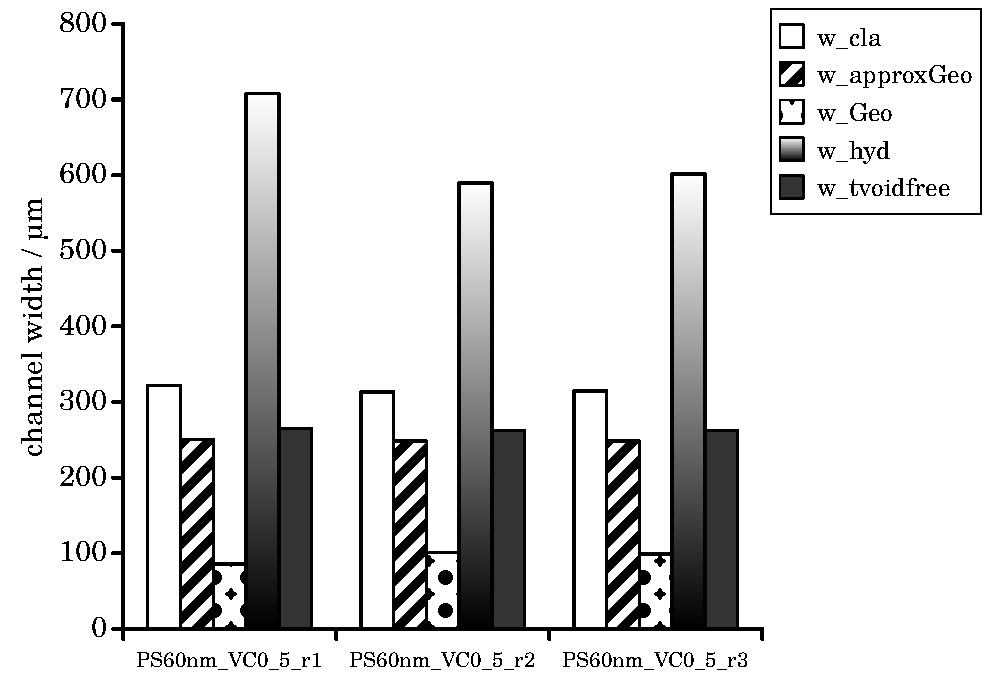
\includegraphics[width=\linewidth]{./images/data/img_calibW_PS_VC_0_5.pdf}
      \subcaption{Calibration results for $w$}
%      \label{subfig:calibRes_PS_VC0_5_w}
    \end{subfigure}
    \begin{subfigure}{\subFigSize}
      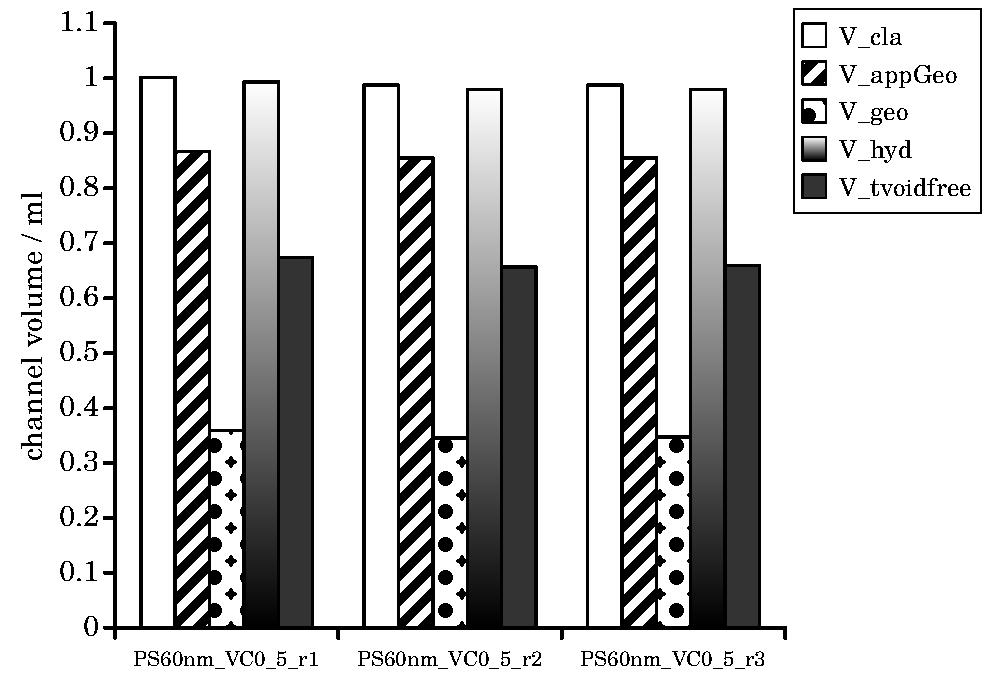
\includegraphics[width=\linewidth]{./images/data/img_calibV_PS_VC_0_5.pdf}
      \subcaption{Calibration results for $V$}
    \end{subfigure}
 \end{center}
  \vspace*{-4ex}    
  \caption[Results of $w$ and $V$ from all 5 calibration algorithms for PS measurements at
  $\Vc = \SI{0.5}{\mlmin}$]{
    Results of $w$ and $V$ from all 5 calibration algorithms for PS measurements at
    $\Vc = \SI{0.5}{\mlmin}$
  }
  \label{fig:calibRes_PS_VC0_5}
\end{figure}
\FloatBarrier
%\clearpage
\newgeometry{margin=1.3cm}
\needspace{20em}
\section*{Deviation influences}
%\lipsum
\begin{figure}[H]
  \begin{center}
    \includegraphics[width=.925\linewidth]{./images/deltaAnalysis.pdf}
  \end{center}
  \vspace*{-3ex}
  \caption[Parameter deviation analysis, example for sample BSA\_VC2\_5\_r1]{Parameter deviation analysis, example for sample 
  BSA\_VC2\_5\_r1}
  \label{fig:DeviationAnalysis}
\end{figure}
\FloatBarrier
\restoregeometry
%\KOMAoptions{paper=a4}
%\recalctypearea
%\clearpage
%\lipsum